%!TEX root = first try.tex  

\chapter{Basic concepts of railway bridge dynamics}

In this chapter some basic concepts of railway bridge dynamics will be described in order to provide preliminary relevant knowledge for following chapters. The knowledge will be introduced in the order of railway related only to bridge related. 

\section{Sources induce transverse dynamic reactions}
According to \cite{da2007dynamic}\cite{fryba1996dynamics}\cite{EC12}, following sources are identified:

\begin{enumerate} [-]
	\item Horizontal track irregularities
	\item Sinusoidal motion of conical wheels along cylindrical rail heads
	\item Centrifugal forces on curved tracks
	\item Train switches
\end{enumerate}

\section{Wheel-Rail Interface}

\subsection{Wheelset and track dimensions}

Generally the track guage is used as a distance measured between the two rails, more specifically the distance between the inside of the railheads measured 14mm below the surface of the rail. By choosing 14 mm the measurement is less influenced by lipping or lateral wear on the rail head and by the radius r = 13 mm of the rail head face. On normal track the gauge is $1435^{+10}_{-3}$ mm with with a maximum gradient of 1:3000. For new track, however, NS apply the following standards:

\begin{enumerate}
\item Mean gauge per 200 m: $1435^{+10}_{-1}$ mm
\item Standard deviation within a 200 m section less than 1 mm
\end{enumerate}

\begin{figure}[h]
\centering
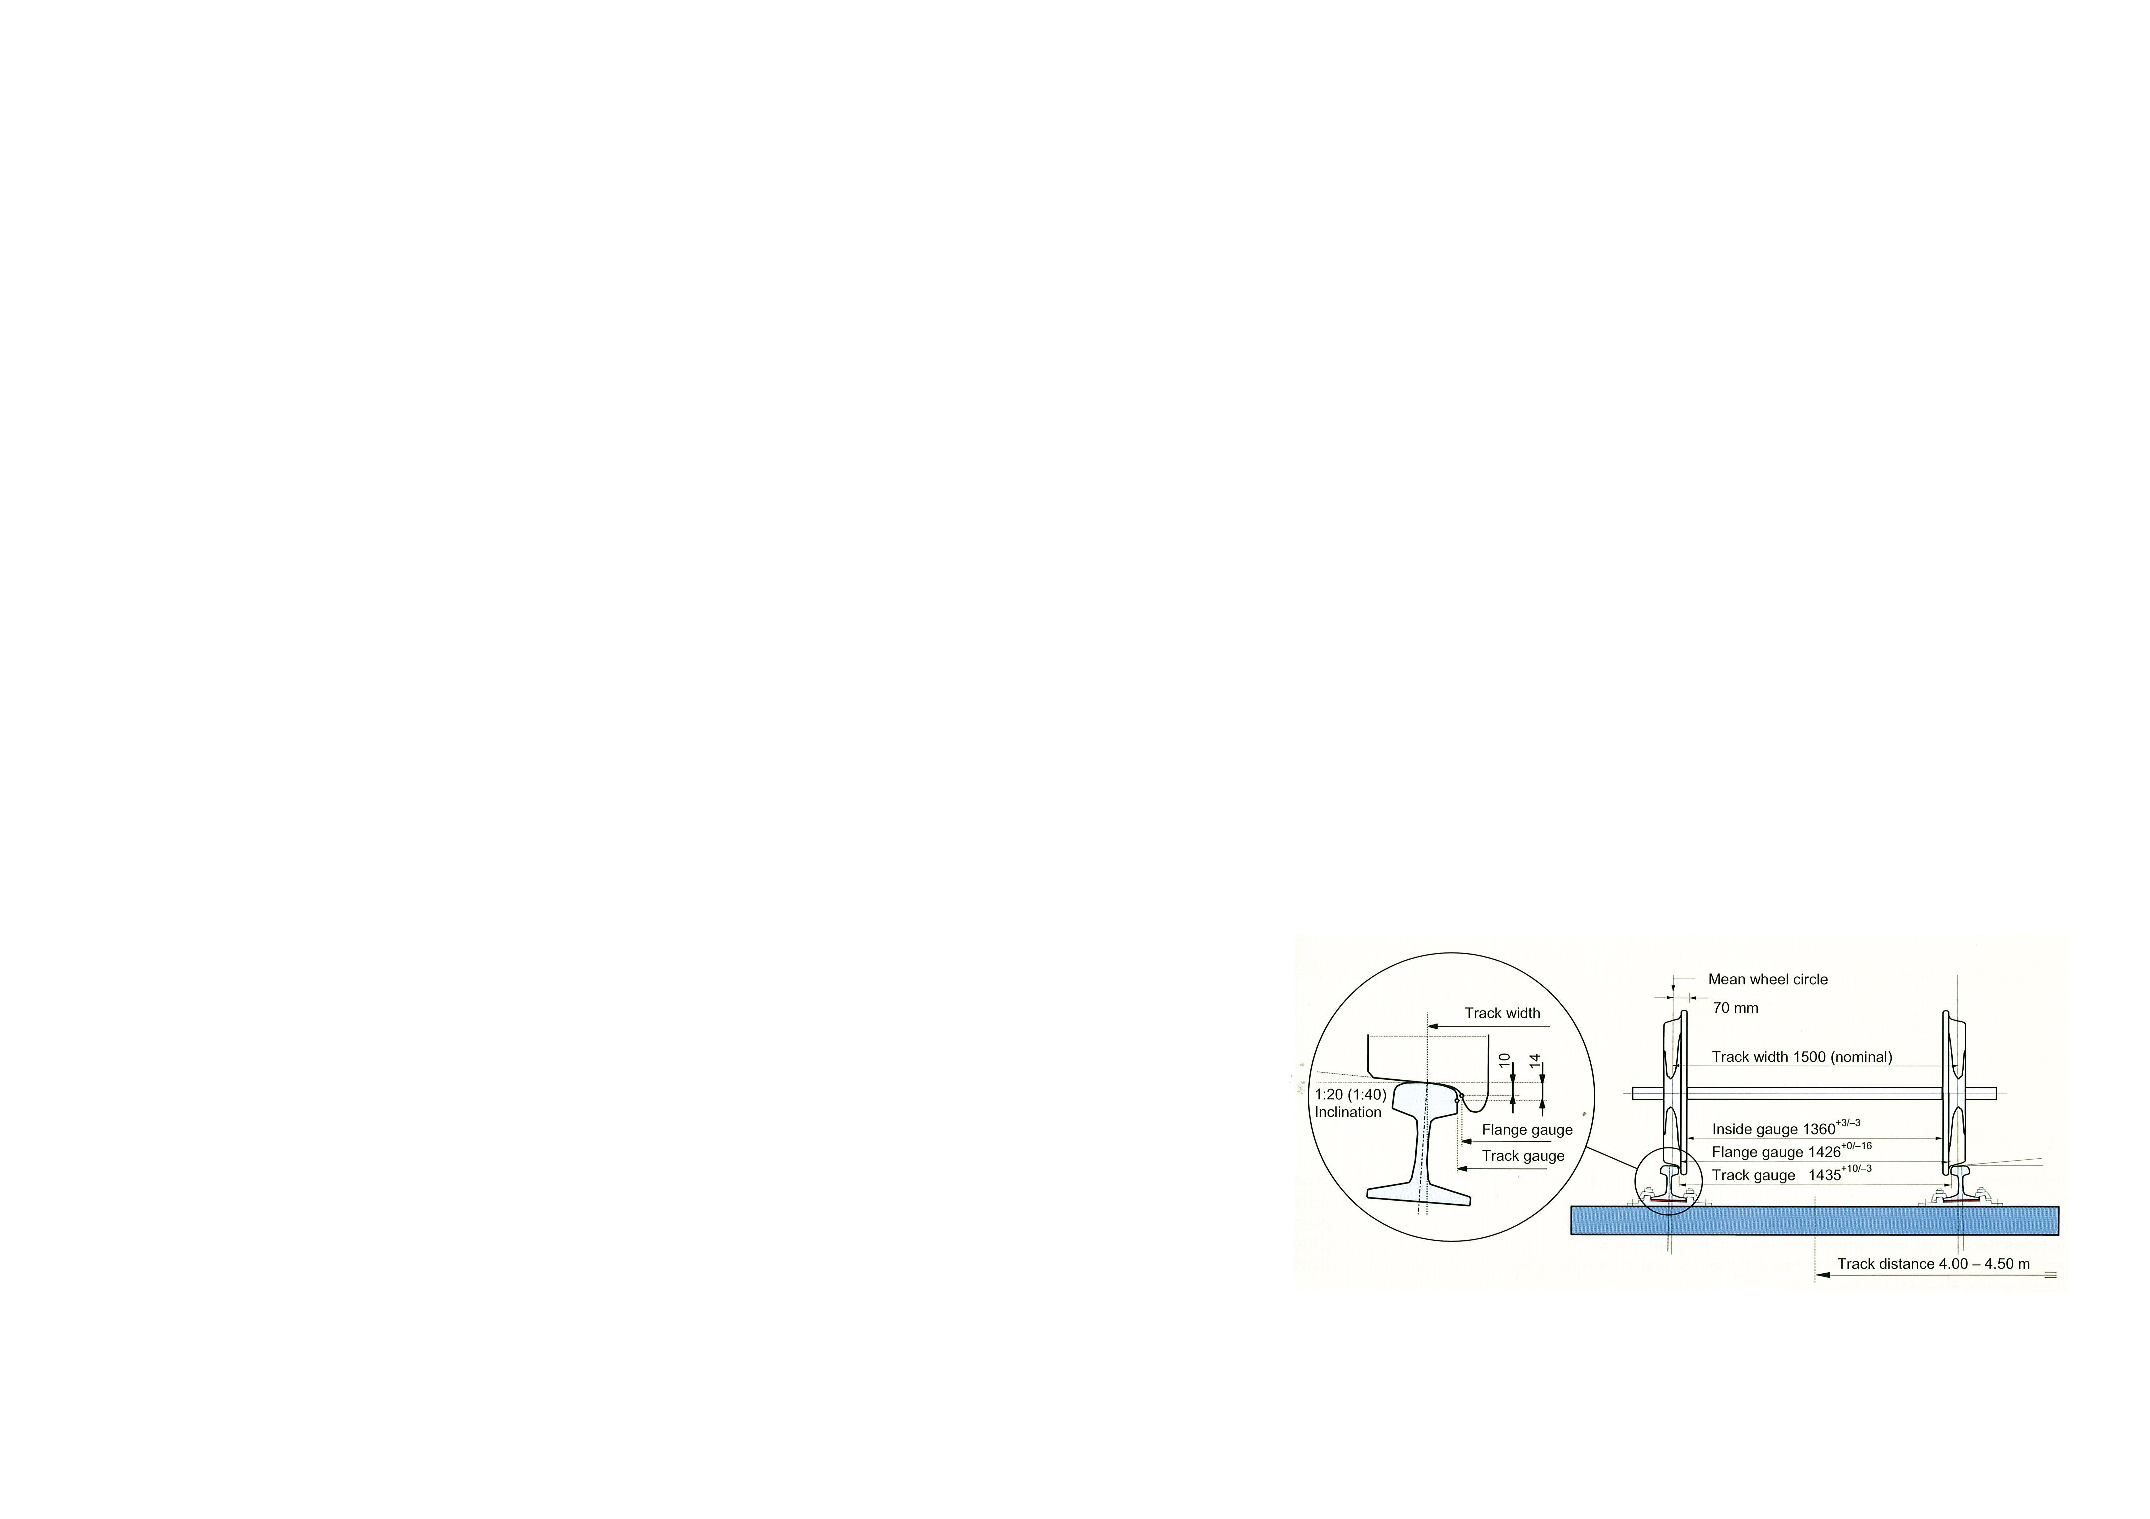
\includegraphics[width=0.8\textwidth]{wheelsettrackdimension.pdf}
\caption{Wheelset and track dimensions for straight normal gauge track. Extracted from \cite[p.17]{esveld2001modern}}
\label{fig:wheelset and track dimensions}
\end{figure}

\subsection{Conicity and Equivalent Conicity of Wheels}

Originally conical tire profiles with an inclination of 1:20 were used. Since a centrally applied load on the railhead is desired, a rail inclination of 1:20, as shown in Figure 2.1, was also selected; this for instance still applies to NS profile NP 46. UIC 54 rail usually has an inclination of 1:40. This inclination matches the S 1002 worn wheel profile which is in general use in Europe. During manufacturing the tires are given a profile which matches the average shape cause by wear. In contrast to the straight conical profile this has a hollow form.

It is clear that regarding a worn profile the conicity depends on the actual shape of the rail head and tire, including any wear, track gauge, and rail inclination. Likewise, elastic deformation of the wheelset and rail fastenings plays a role.

Generally, the effective or equivalent conicity is defined as:

$$ \gamma_e = \frac{\Delta r}{2y} = \frac{r_1 - r_2}{2y}  $$

Here $r_1 - r_2$ is the instantaneous difference in rolling radius of the wheel treads; generally speaking this is a non-linear function of the lateral displacement y of the wheelset with respect to the central position. The difference between conical and worn profiles is given in Figure.\ref{fig:conicalwornprofiles}. To enable numerical comparisons $\gamma_e$ is determined at a certain lateral displacement $y=\bar{y}$.

\subsection{Worn wheel profiles}

A perfectly conical wheel profile is unstable as far as its shape is concerned, but will take on a shape that is stable as the effect of wear.

Practical research has shown that over a period of time wheel profiles stabilise with wear at an equivalent conicity of 0.2 to 0.3. With regards to running stability, the equivalent conicity must remain below 0.4 and to ensure the centering effect it must be greater than 0.1.

\begin{figure}[h]
    \centering
    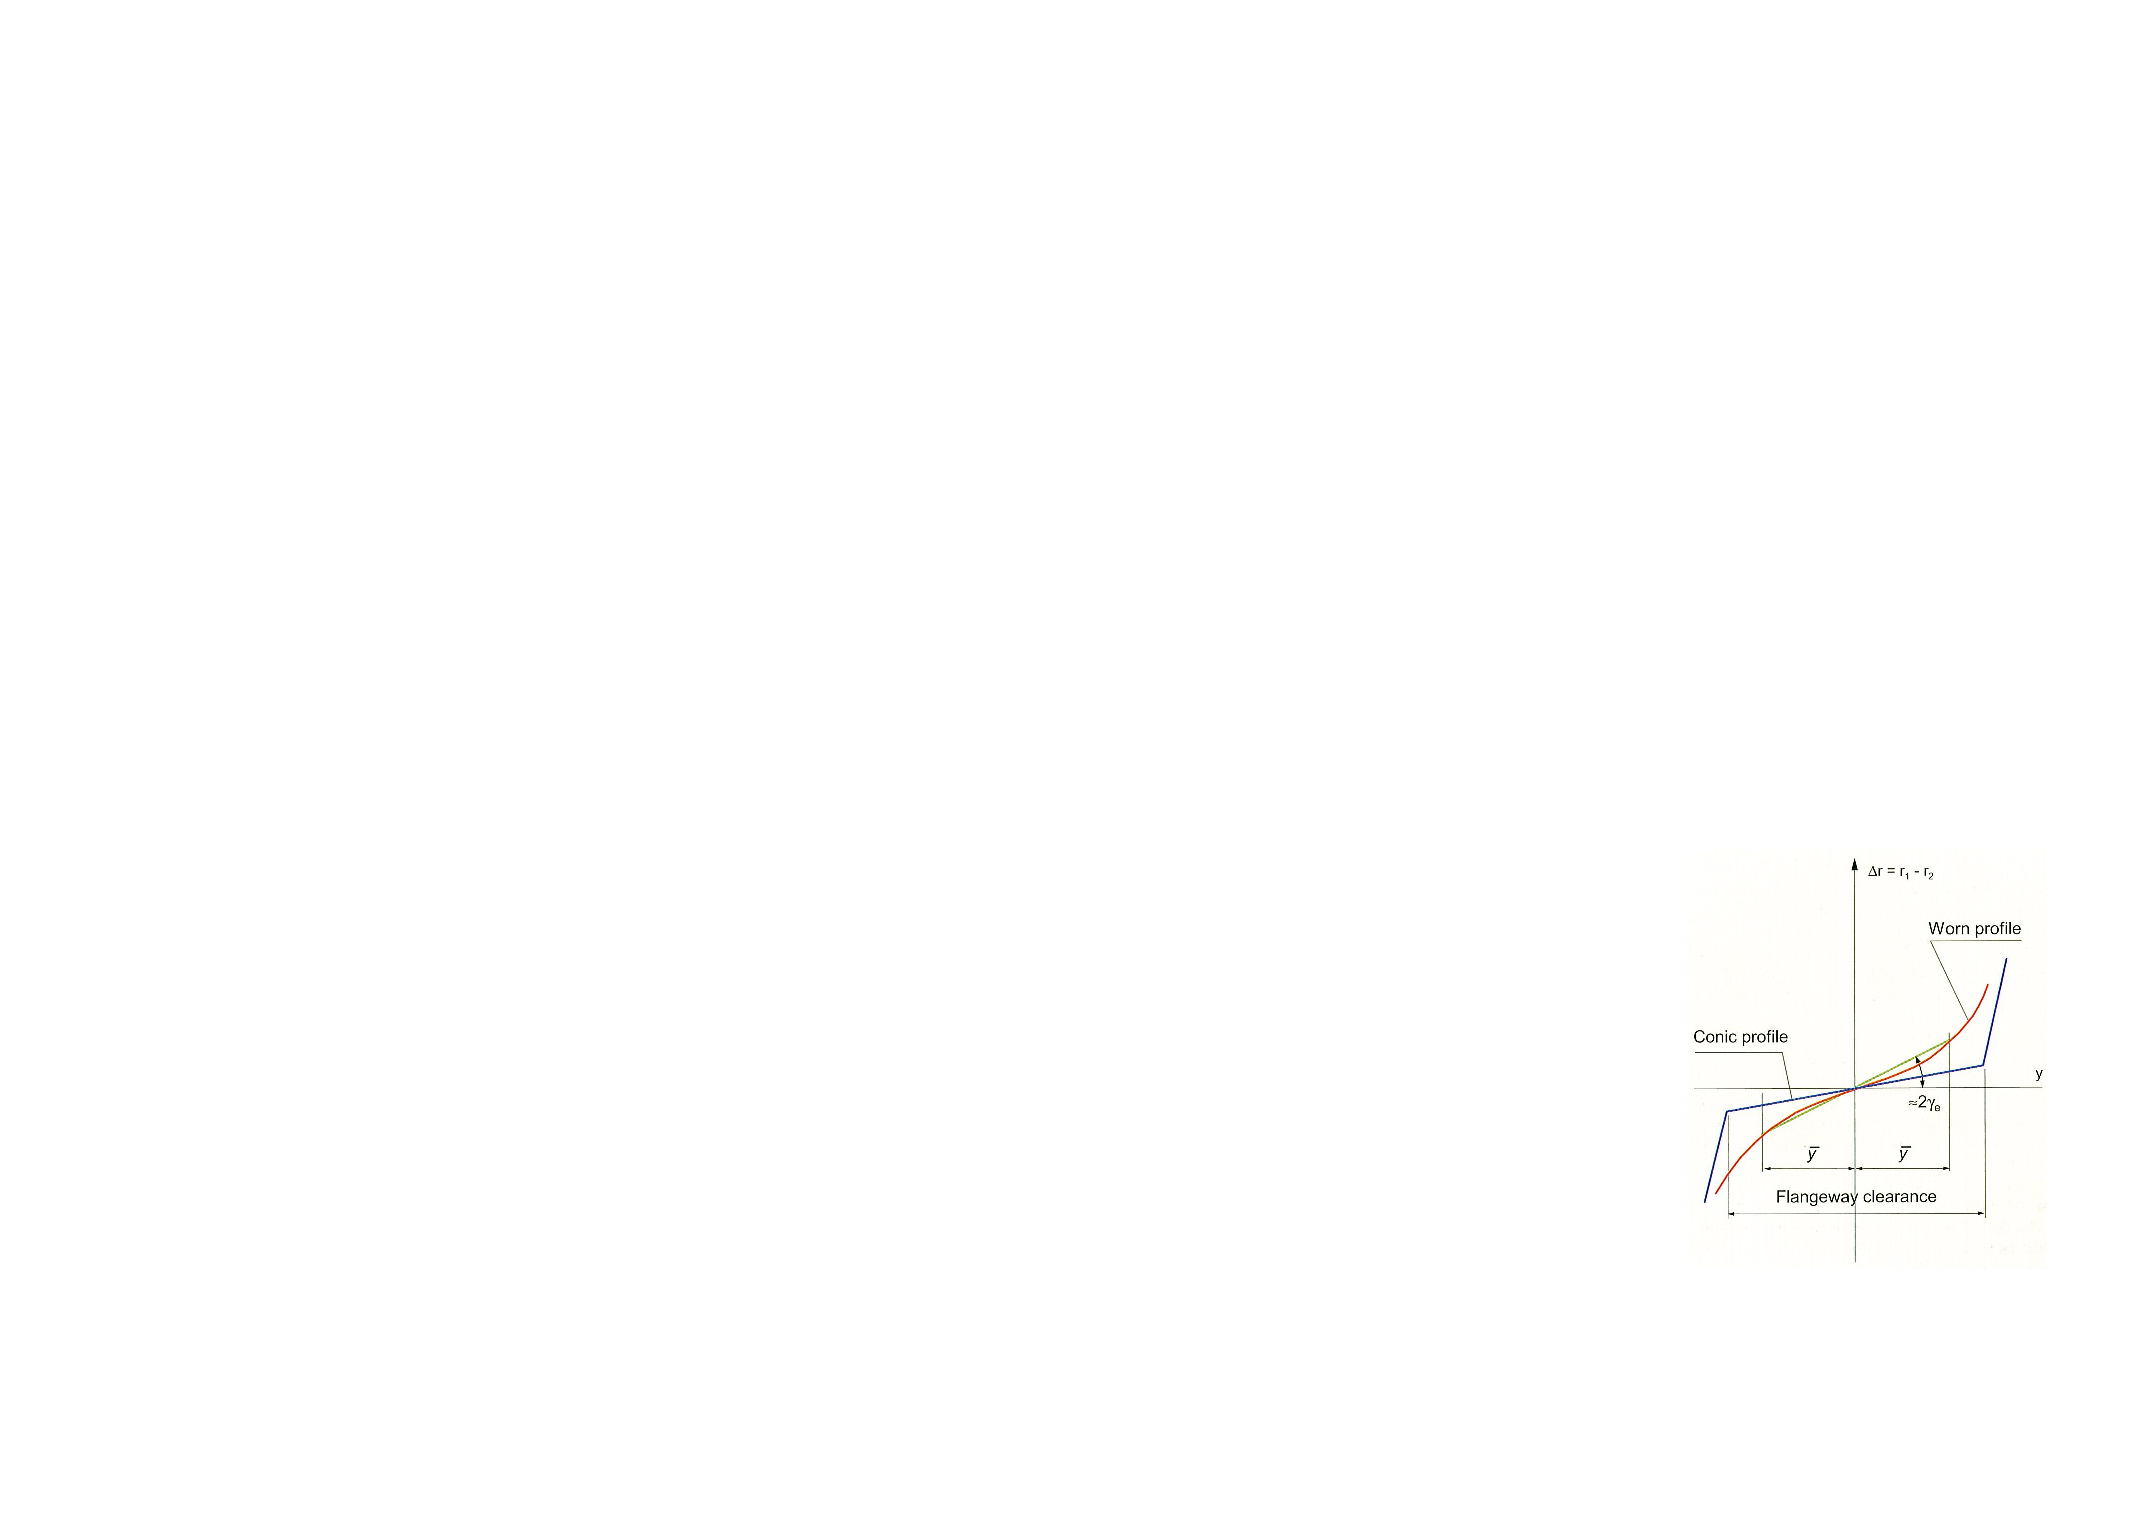
\includegraphics[width=0.6\textwidth]{conicalwornprofiles.pdf}
    \caption{$y-\Delta r$ curves. Difference between conical and worn wheel profiles. Extracted from \cite[2.4]{esveld2001modern}}
    \label{fig:conicalwornprofiles}
\end{figure}

With a conical profile the conicity is constant and above equation becomes:

$$ \gamma_e = \frac{\Delta r}{2y} =\frac{(r+\gamma y)-(r-\gamma y)}{2y} = \gamma $$

\subsection{Lateral Track Irregularities}\label{sec:lateraltrackirrgularities}
This section describes allowable lateral track irregularities defined in EN13848-5\cite{13848}. 

Lateral alignment irregularities was defined in EN13838-1. It states:"Deviation $y_p$ in y-direction of consecutive positions of point P... on any rail, expressed as an excursion from the mean horizontal position (reference line) covering the wavelength ranges stipulated below and calculated from successive measurements ...". See Figure \ref{fig:lateraldeviationdefine}.

For lateral deviations, the following wavelengths shall be considered: $D1 = 3 -25 m$, $D2 = 25 - 70 m$ and $D3 = 70 - 200 m$. 

\begin{figure}[h]
    \centering
    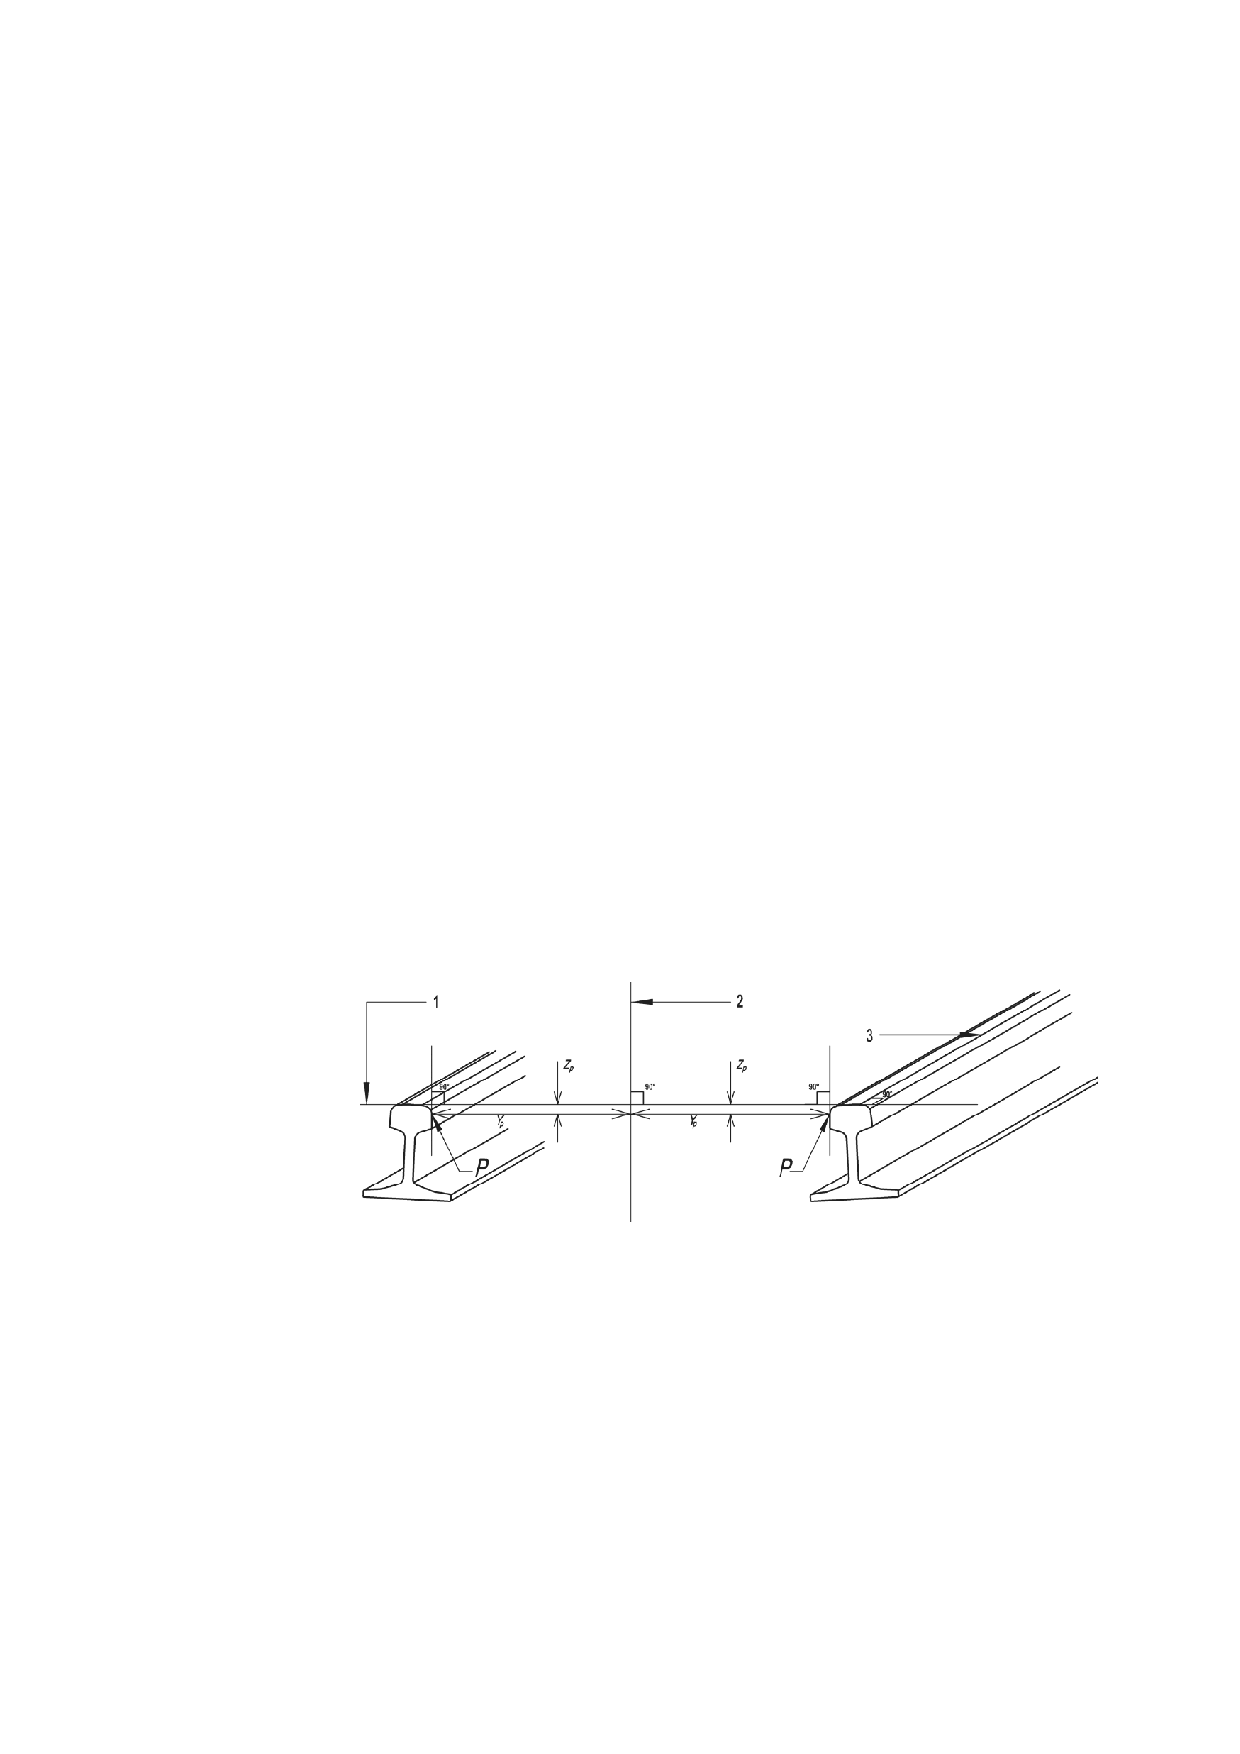
\includegraphics[width=0.8\textwidth]{lateraldeviationdefine}
    \caption{Lateral deviation definition. Lateral deviations $y_p$ for each rail with 1: running surface, 2: reference line and 3: centre line of running table}
    \label{fig:lateraldeviationdefine}
\end{figure}

Table \ref{tab:lateraldeviation} defines the allowable standard deviation for lateral track irregularities. Lateral track irregularity has great influence on vehicle's lateral dynamic behaviour.

\begin{table}[h]
    \centering
    \caption{Alignment - AL - Standard deviation. Extracted from \cite[Table B.6]{13848}}
    \begin{tabular}{cc}
        \hline
        Speed(km/h) & Standard deviation(mm) \\
        \hline
        $V\leq 90$ & 1.5 to 1.8 \\
        $80 < V \leq 120$ & 1.2 to 1.5 \\
        $120 < V \leq 160$ & 1.0 to 1.3 \\
        $160 <V \leq 230$ & 0.8 to 1.1 \\
        $230 <V \leq 300$ & 0.7 to 1.0 \\
        \hline
    \end{tabular}
    \label{tab:lateraldeviation}
\end{table}

\section{Lateral movement of a wheelset on straight track}

\subsection{Theory according to Klingel}

If a wheelset with conical tire profiles is laterally displaced from central position, this displacement is counteracted due to different rolling radii of the wheels. This results in a periodical movement of the wheelset which was described by Klingel in 1883 and is therefore often referred to as the Klingel movement. When analysing the case, the wheelset is modelled as a biconus travelling on an ideally straight track as shown in Figure.\ref{fig:wheelsetbiconus}

\begin{figure}[h]
	\centering
	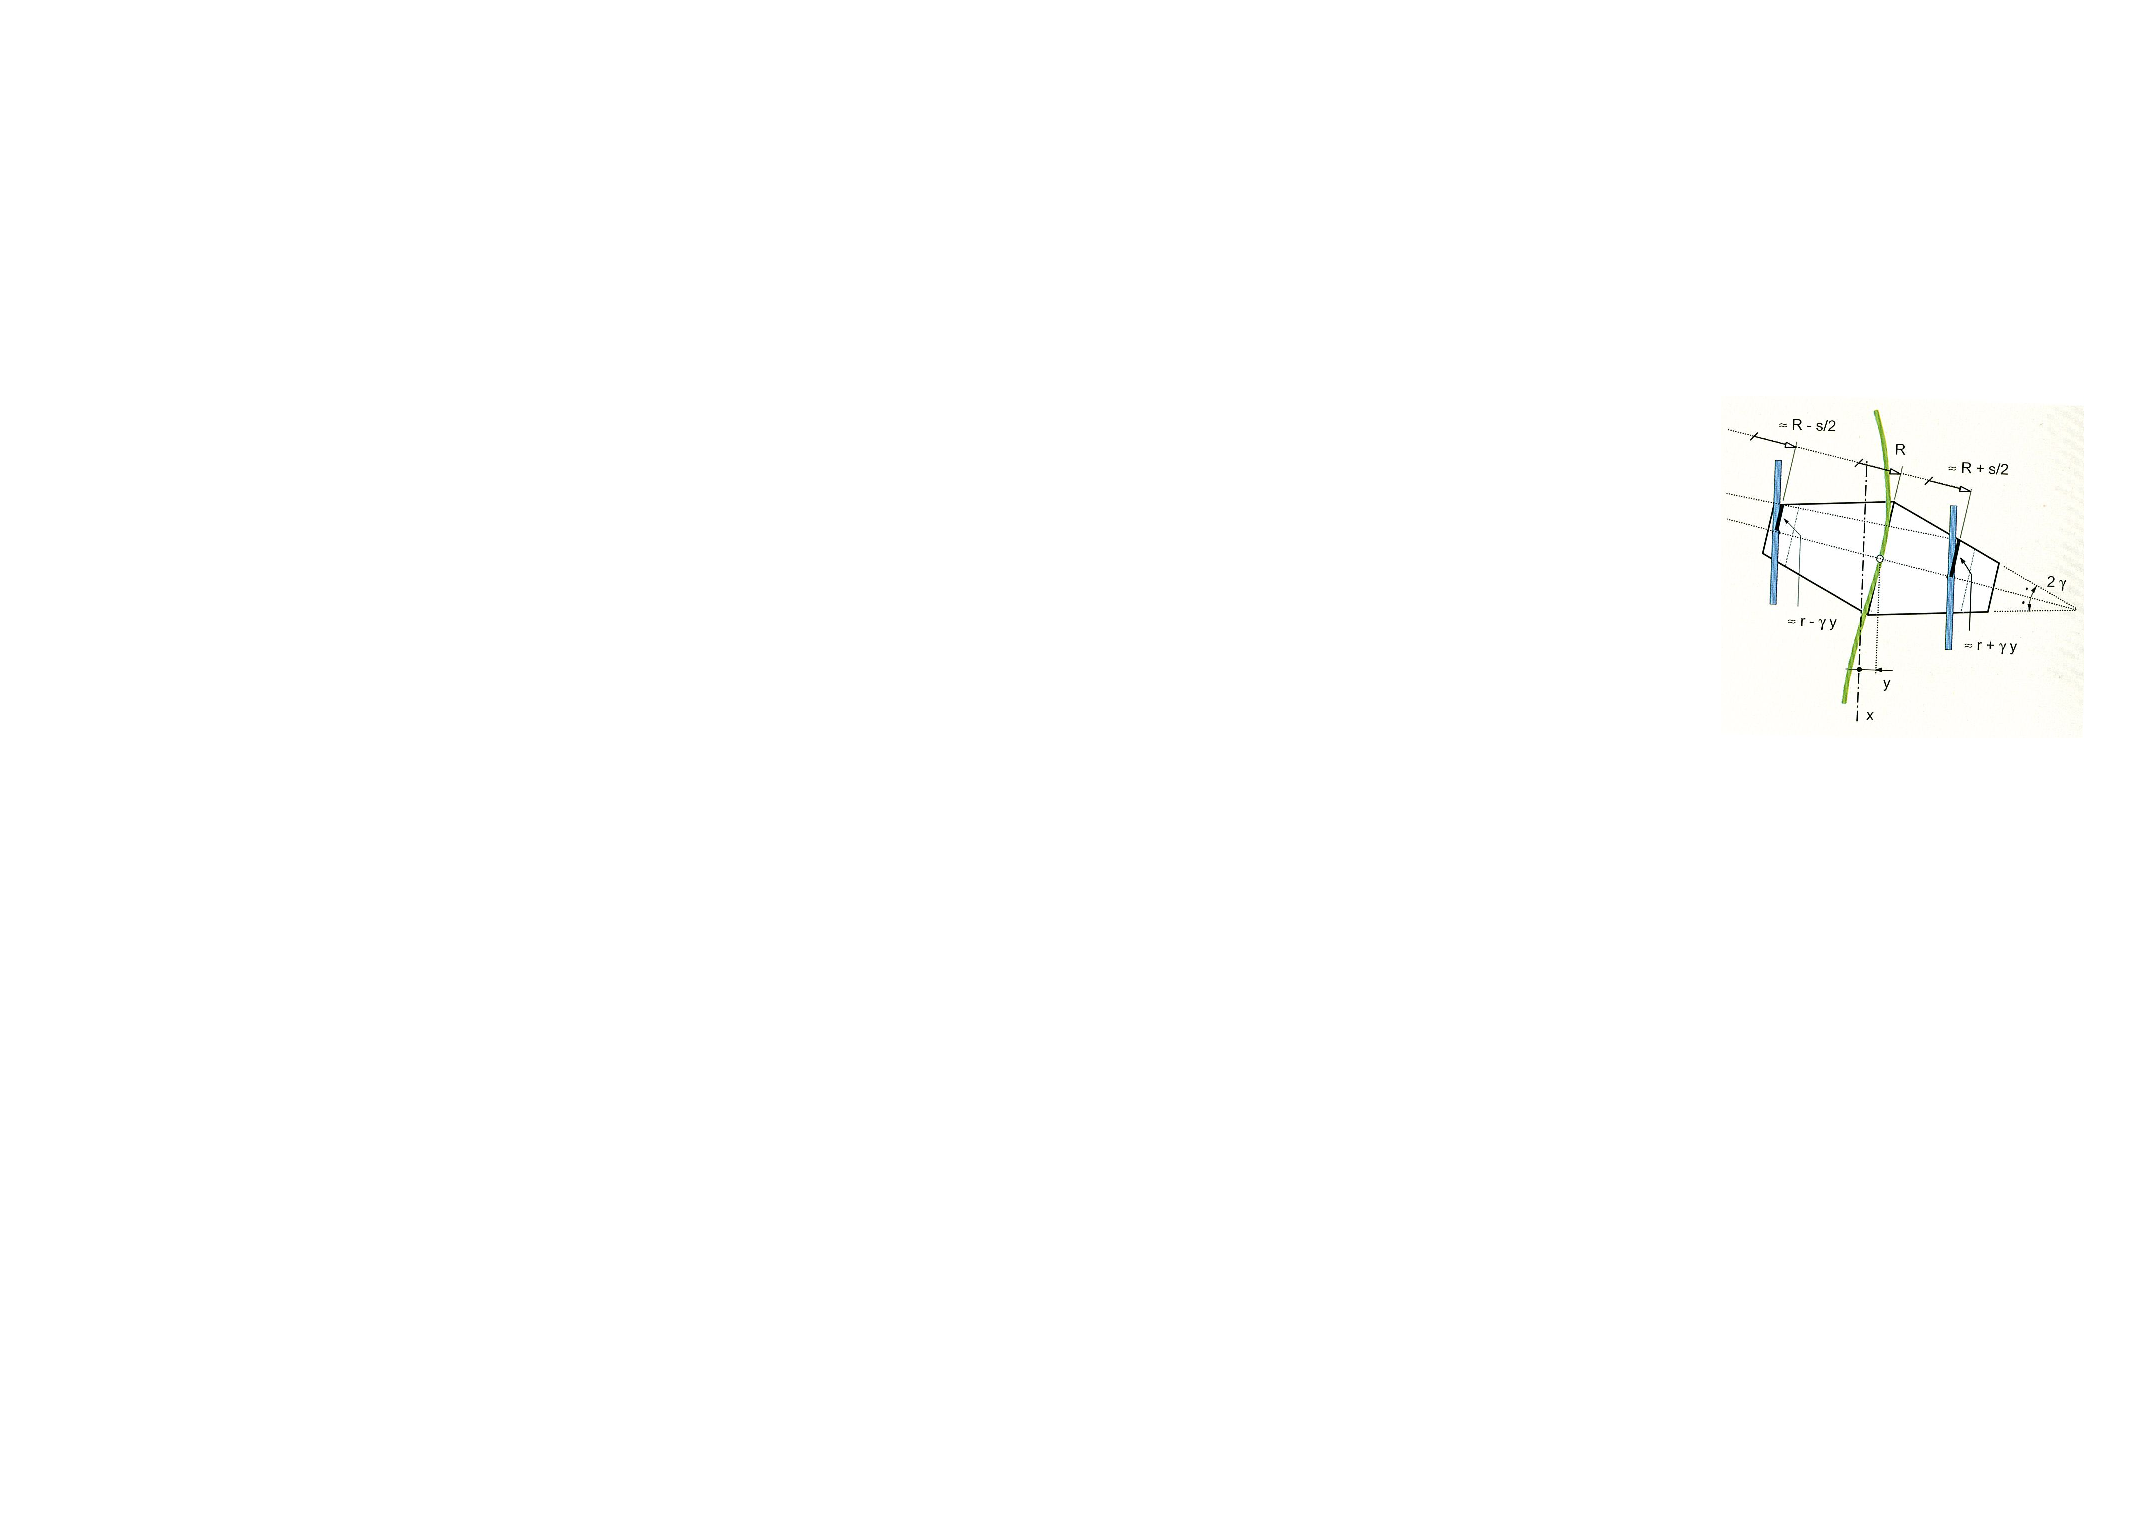
\includegraphics[width=0.5\textwidth]{wheelsetbiconus}
	\caption{Wheelset biconus in general position. Extracted from \cite[Figure 2.2]{esveld2001modern}}
	\label{fig:wheelsetbiconus}
\end{figure}


The Klingel movement is therefore purely a kinematic movement in which forces play no part in the derivation. As a result, Figure.\ref{fig:klingelmovement} visualizes the Klingel movement. The lateral displacement $y$ is a harmonic, undamped function of the distance co-ordinate $x$ as long as the amplitude moves within the flangeway clearance $fwc$. This is illustrated in Figure.\ref{fig:fwc}.

\begin{figure}[h]
	\centering
	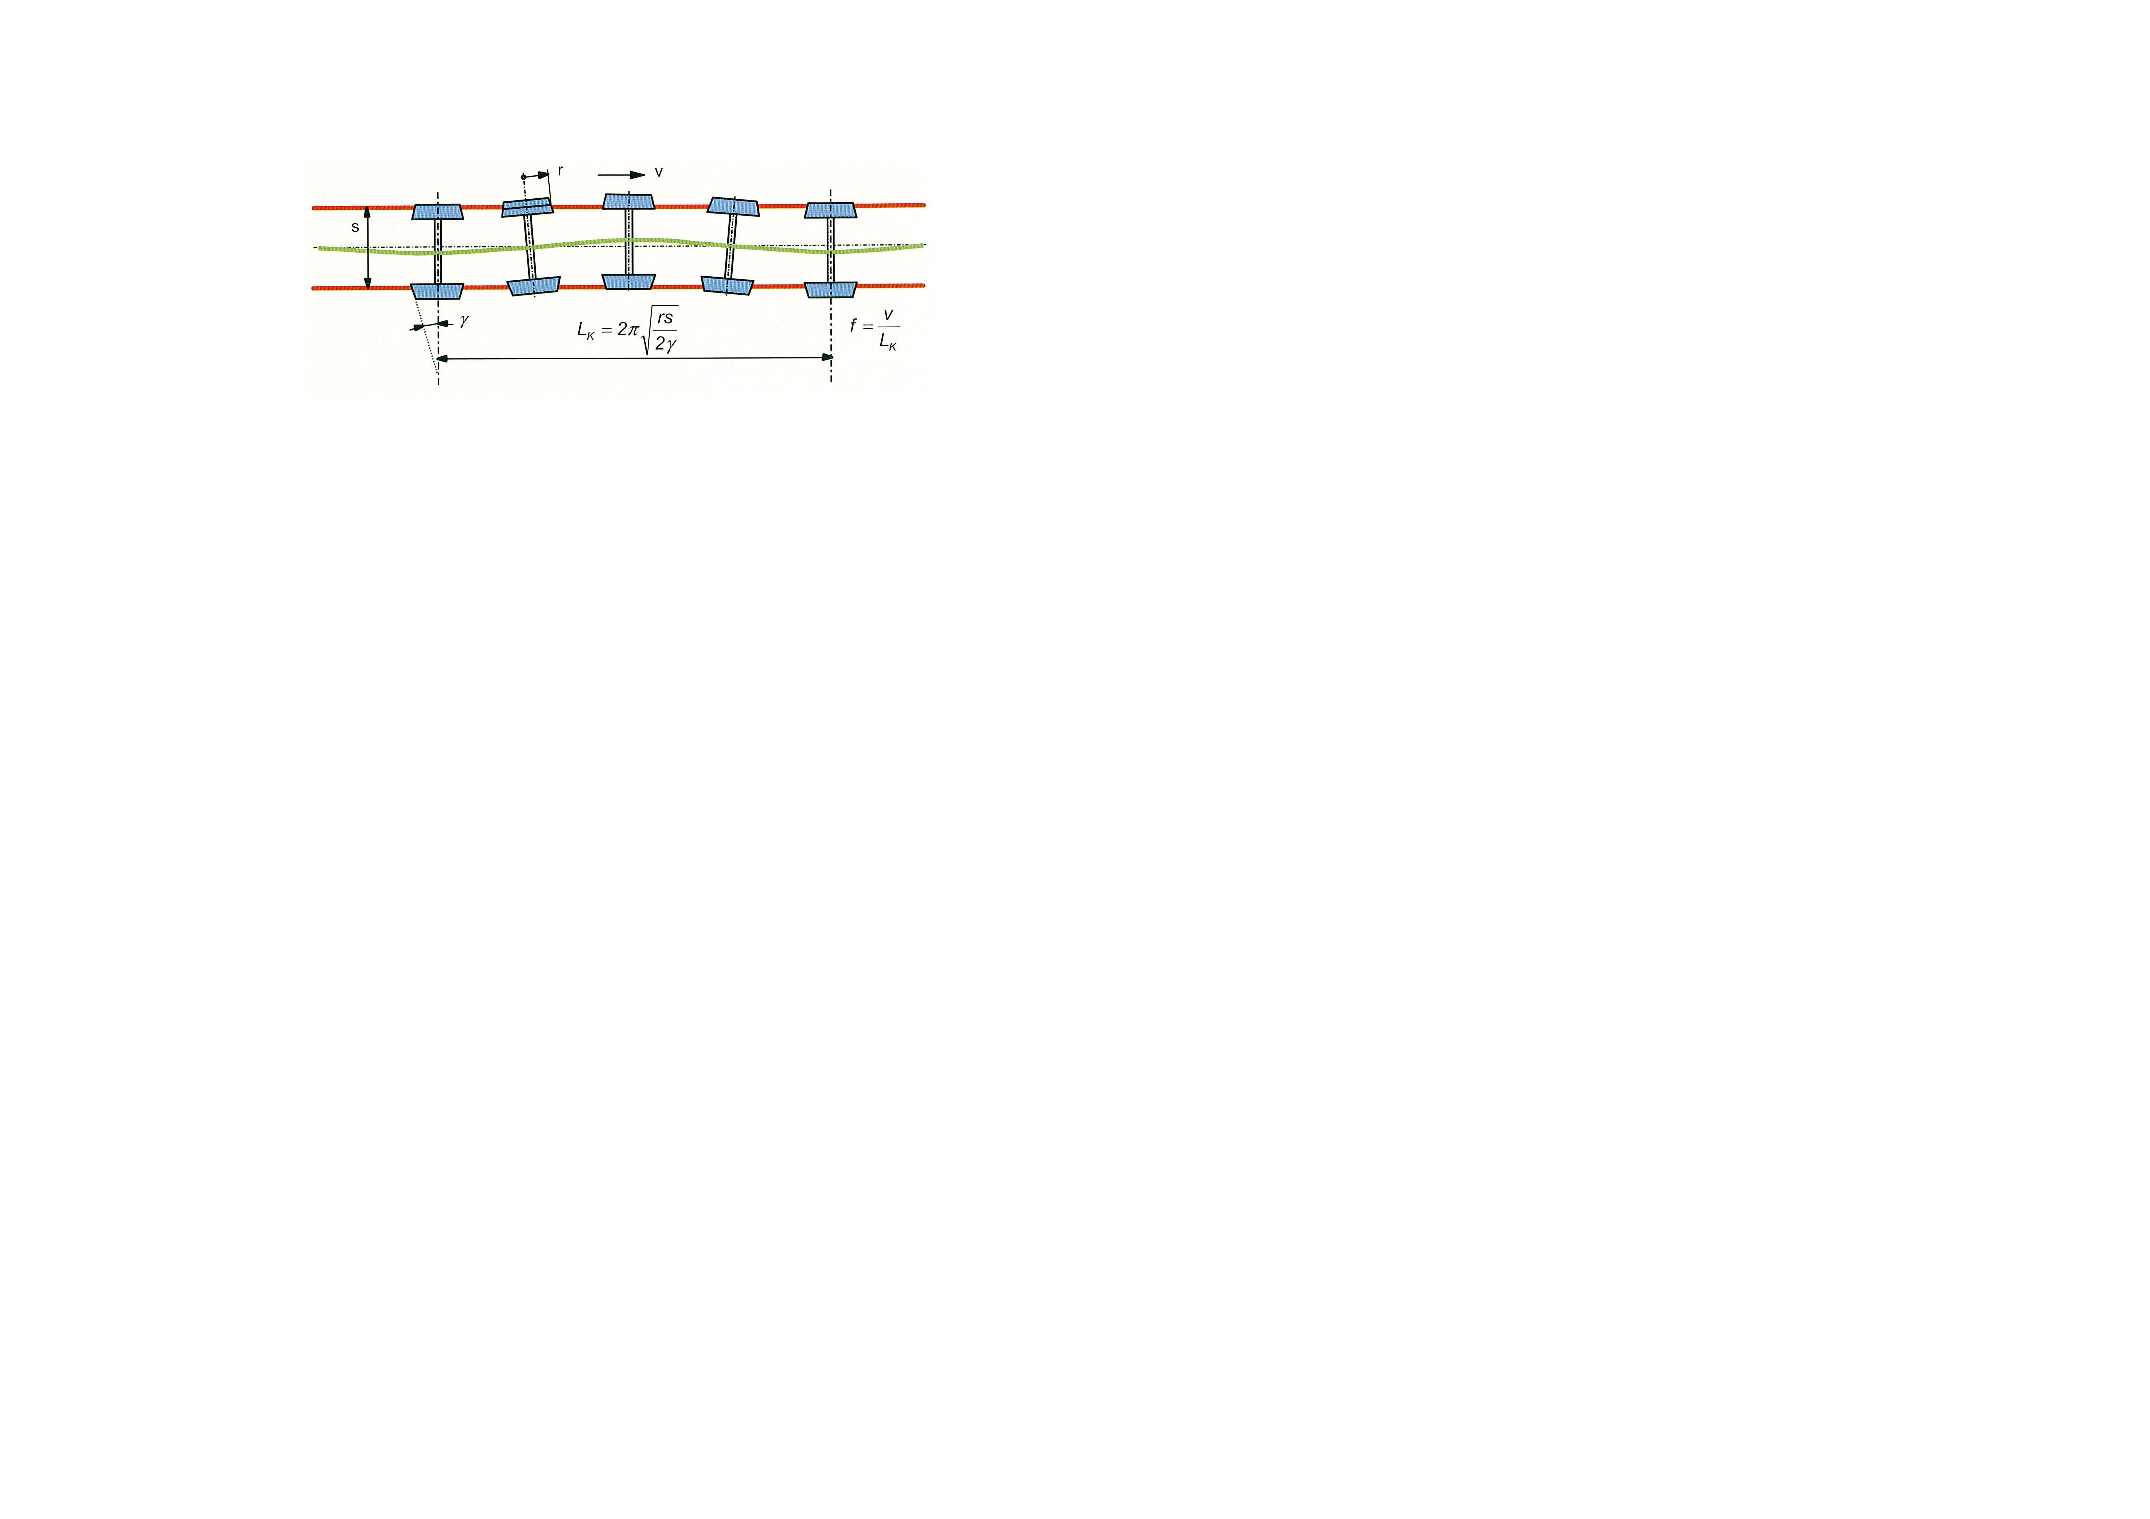
\includegraphics[width=0.8\textwidth]{klingelmovement}
	\caption{Klingel movement. Extracted from \cite[Figure 2.3]{esveld2001modern}}
	\label{fig:klingelmovement}
\end{figure}

\begin{figure}[h]
	\centering
	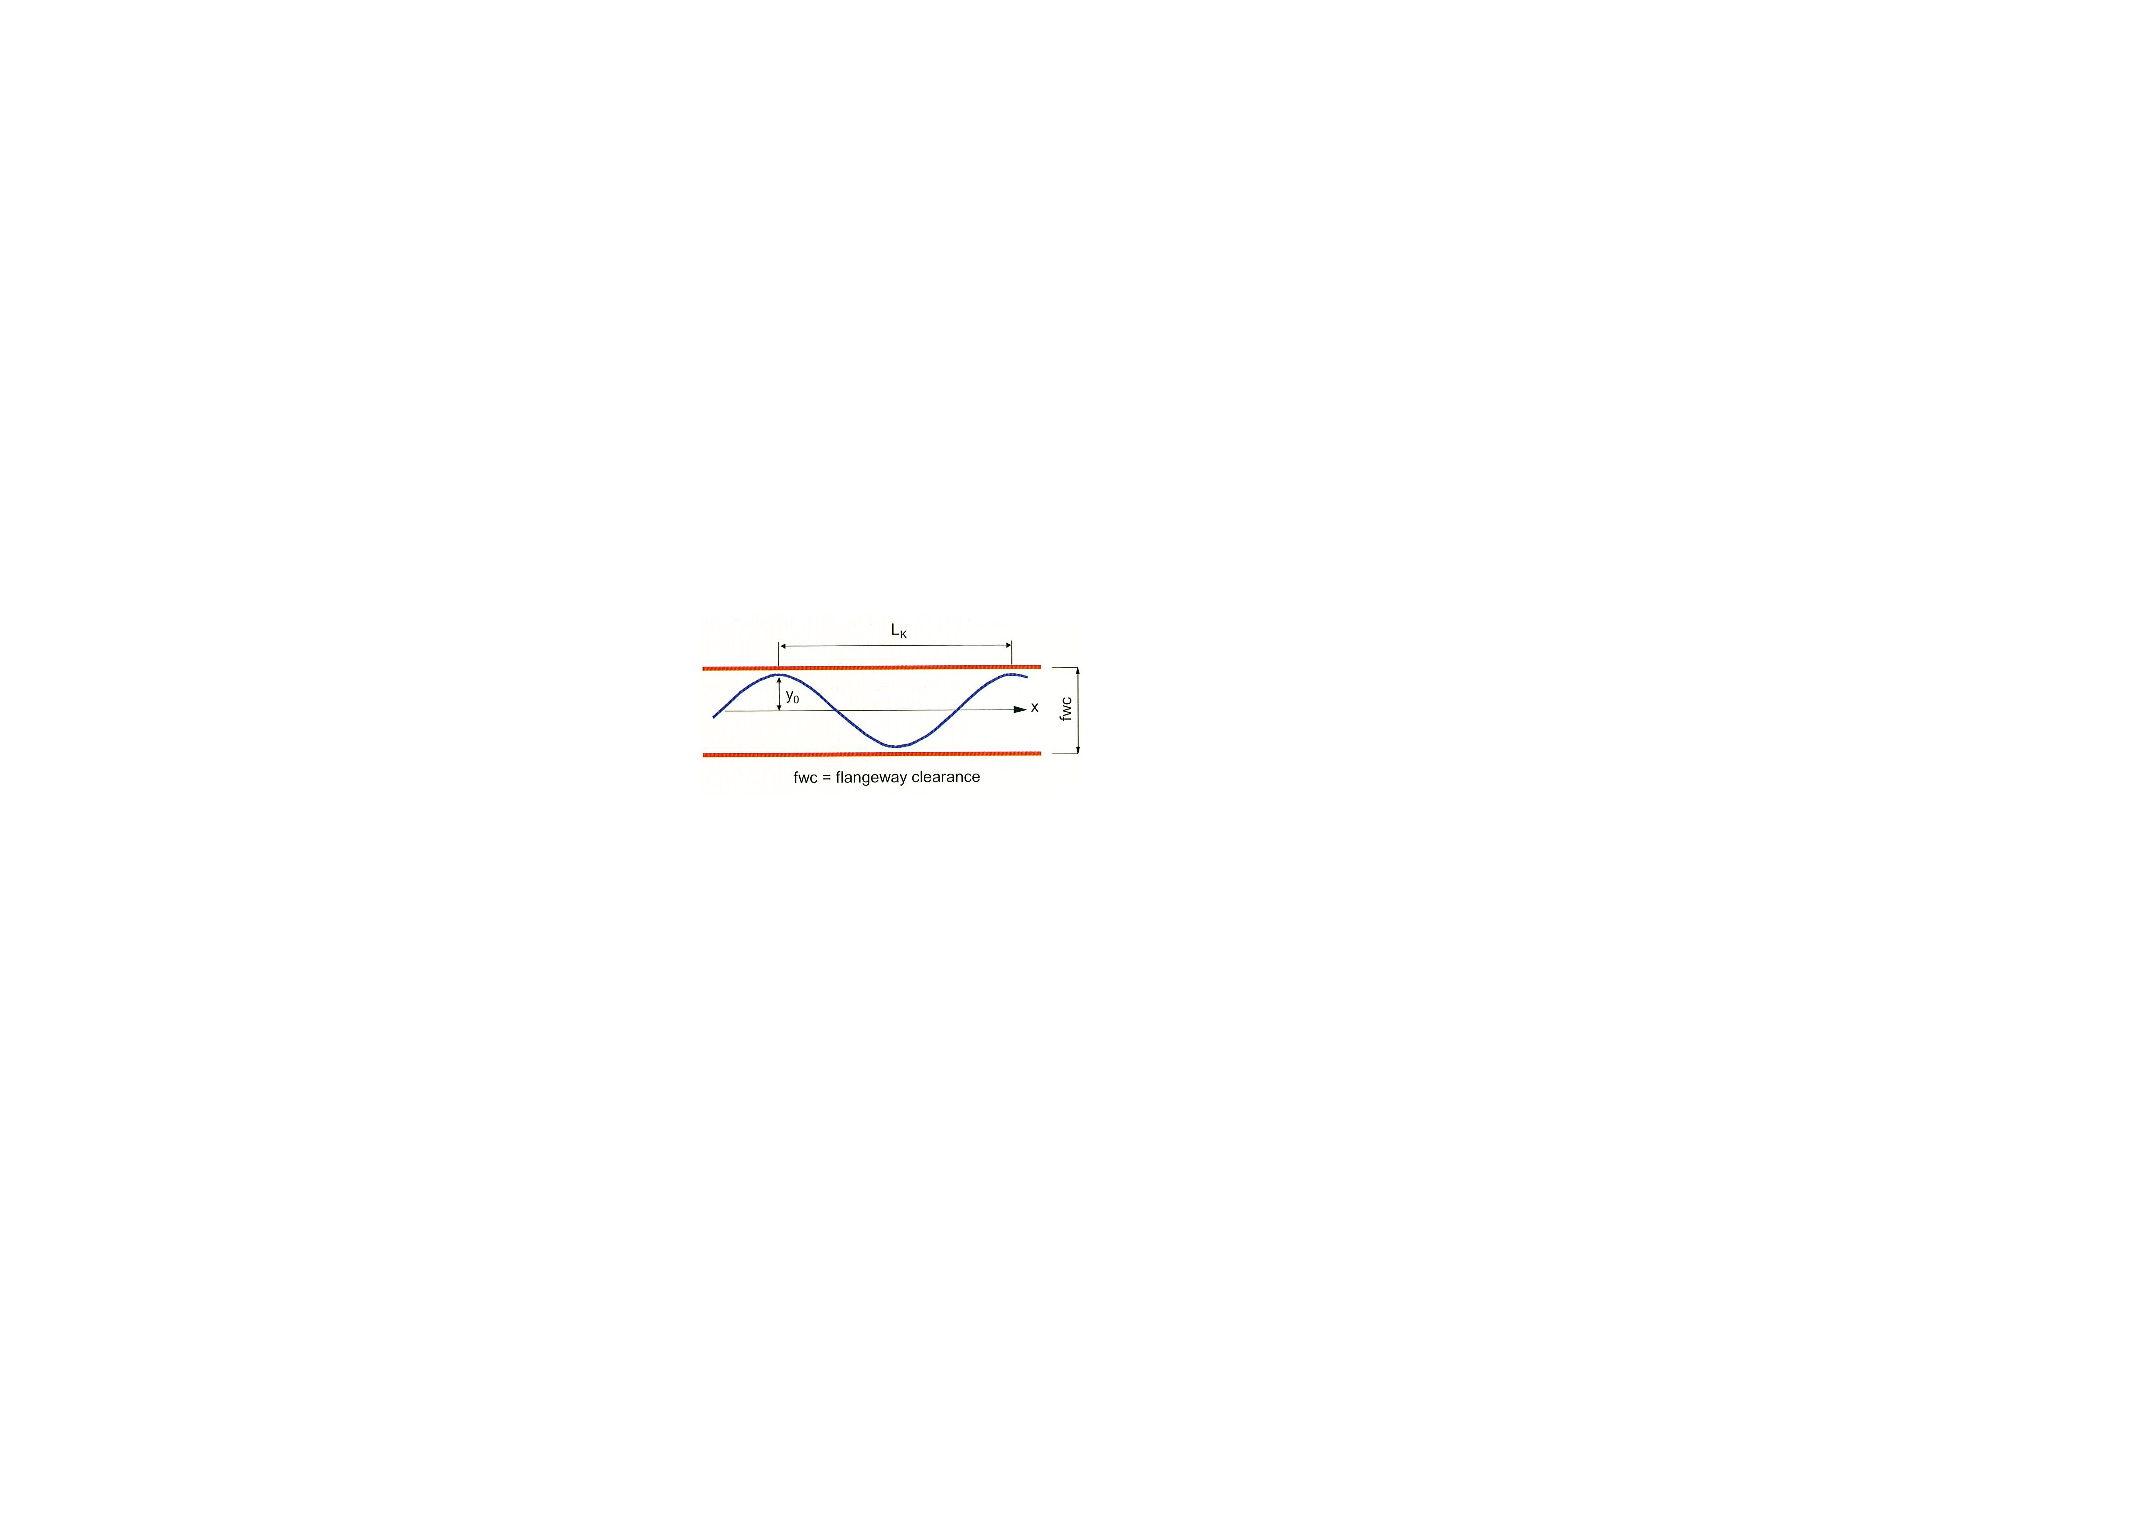
\includegraphics[width=0.5\textwidth]{fwc}
	\caption{Undisturbed lateral movement of a wheelset. Extracted from \cite[Figure 2.4]{esveld2001modern}}
	\label{fig:fwc}
\end{figure}

Introducing the speed, the time domain frequency of the Klingel movement is:

$$ f = \frac{V}{L_k} $$

and hence the maximum lateral acceleration can be calculated as:

$$\ddot{y}_{max} = 4\pi^2y_0\frac{v^2}{L_k^2}$$

If the frequency $f$ coincides with one of the natural frequencies of the rolling stock, the vehicle ride becomes unstable. The lateral acceleration, which is a measure of the forces, shows the adverse effect of high speed and/or small wavelength. A conicity, for example, of 1:40 in comparison with 1:20 therefore gives a greater wavelength and a lower lateral acceleration at the same speed. The progressively increasing conicity in the case of worn profiles due to increasing lateral axle movement, therefore, has an adverse effect in this respect.

\subsection{Hunting movement}

It should be noted that the Klingel theory is simple and instructive but does not include the effect of coupled axes, mas forces, and adhension forces. In reality, the amplitude $y_0$ of the Klingel movement is dependent on alignment, dynamic vehicle behaviour, and the speed of the rolling stock. 

Generally speaking, $y_0$ due to slip will increase with speed until it is equal to half the flangeway clearance. Flanging then occurs as a result of which the axle will rebound. 

This means that the lateral movement takes on a completely different behaviour which is known as hunting. As shown in the drawing in Figure\ref{fig:flangingwheelset} the movement changes from a harmonic to a zig-zag shape. The wavelength becomes shorter and the frequency increases quickly until it is in the critical range for the rollin g stock and resonance occurs.

\begin{figure}[h!]
	\centering
	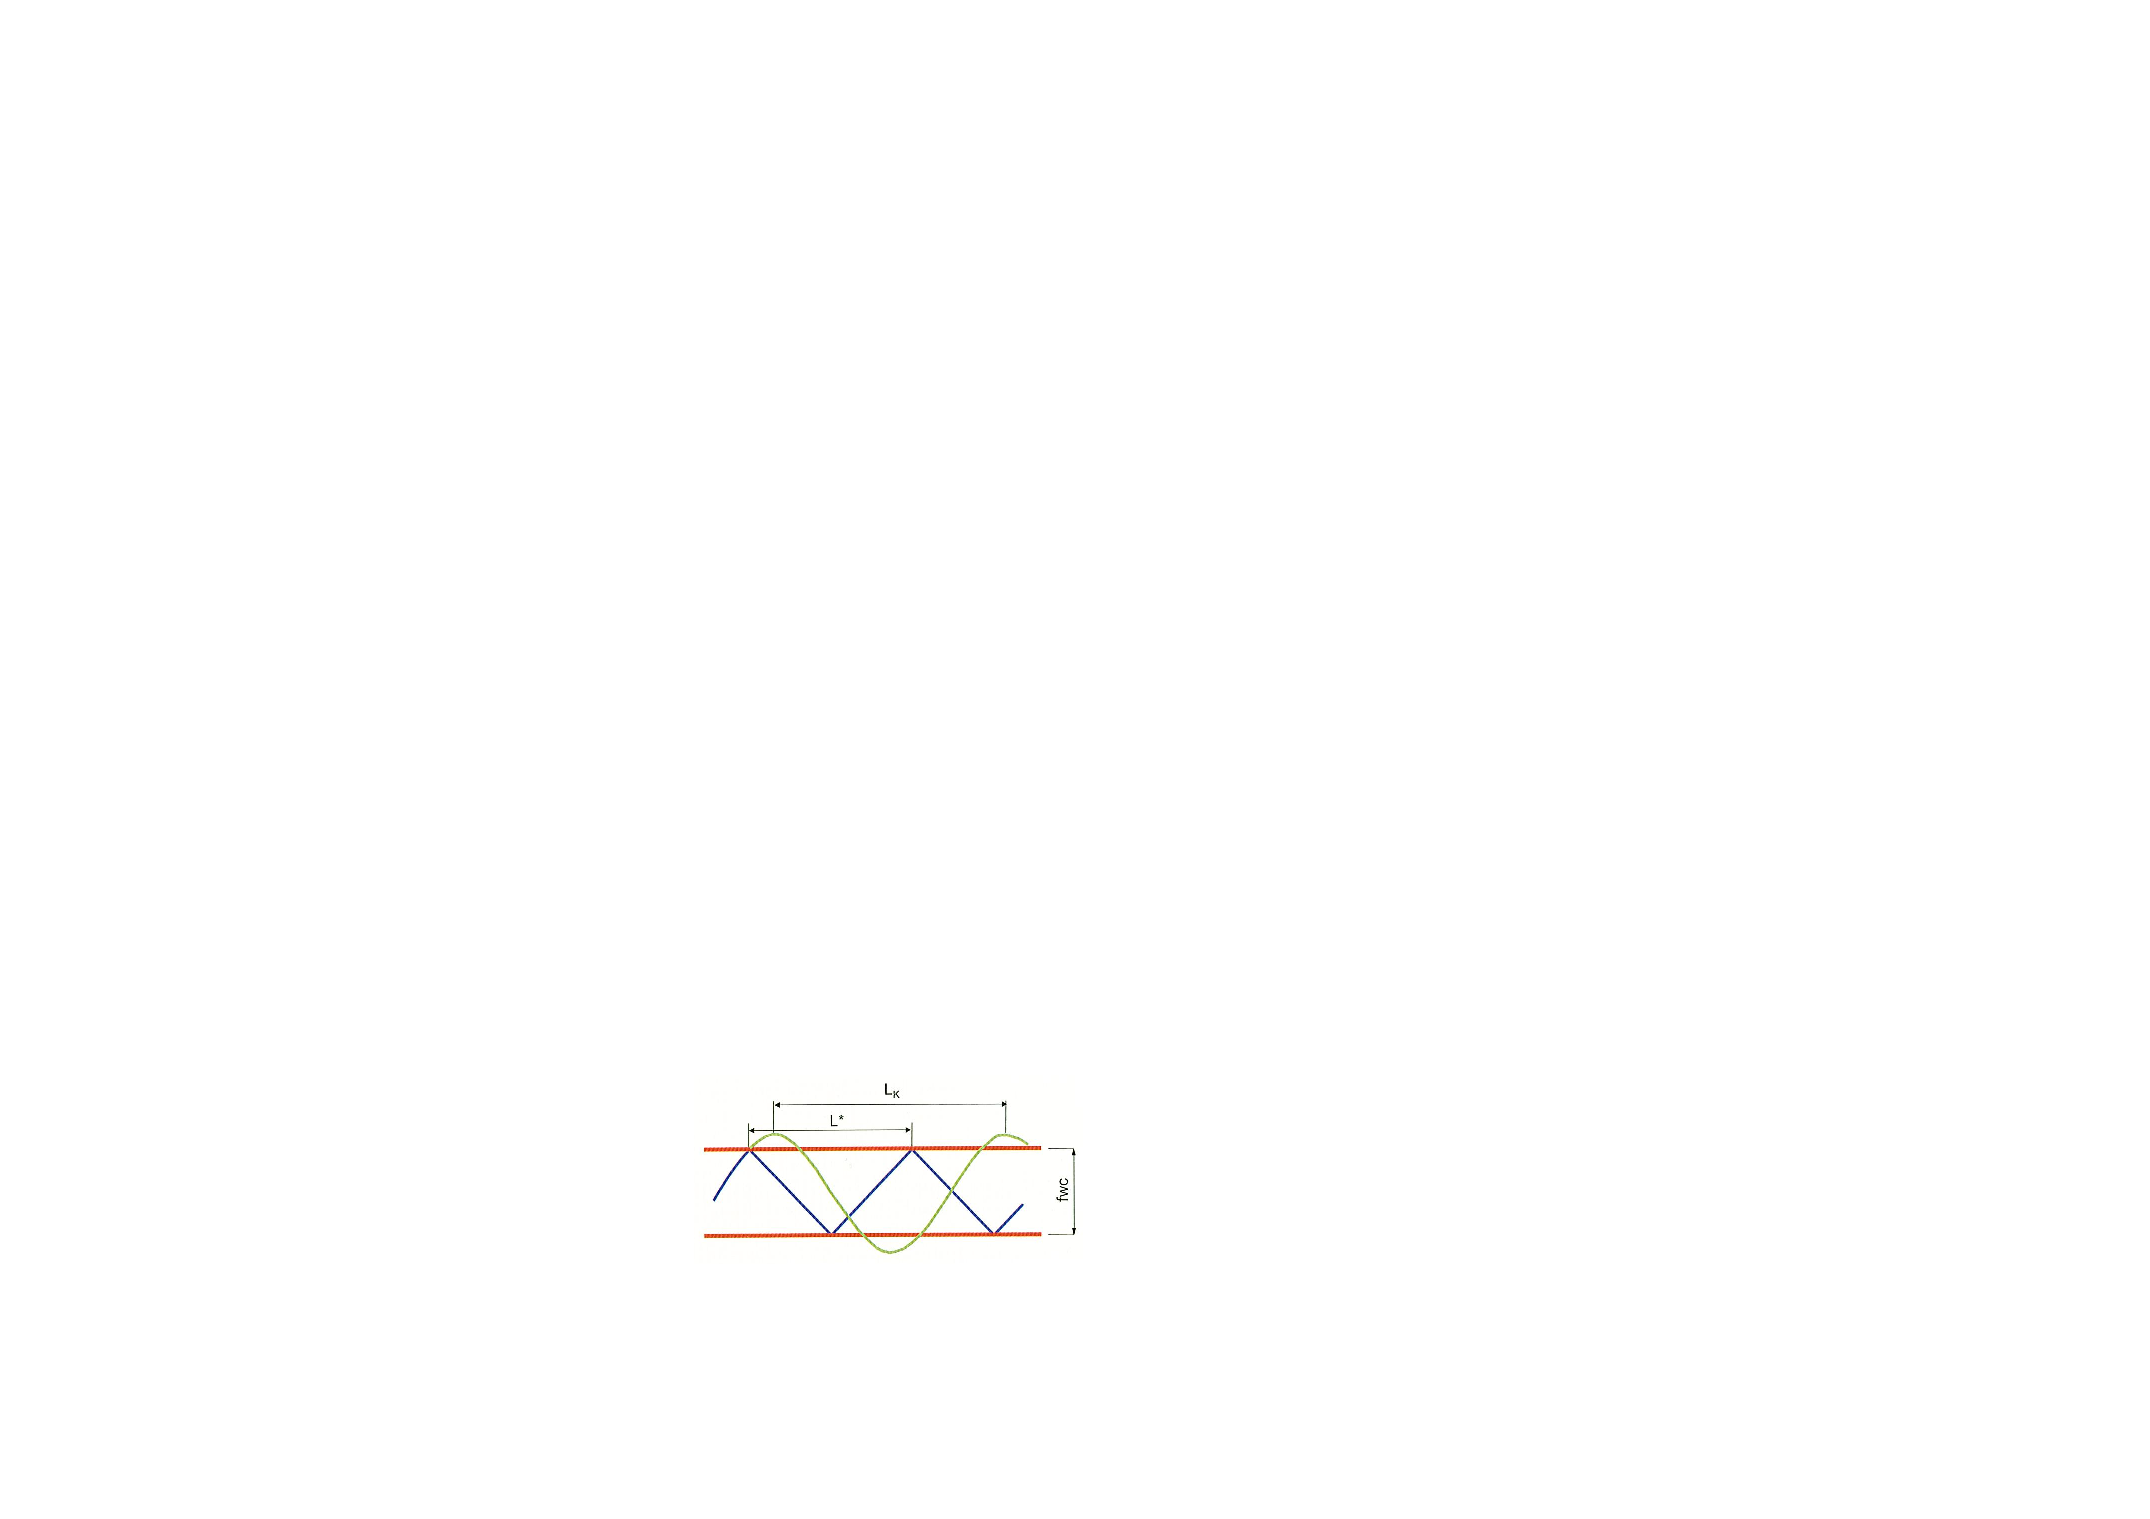
\includegraphics[width=0.5\textwidth]{flangingwheelset}
	\caption{Influence of flanging on lateral wheelset movement. Extracted from \cite[Figure 2.5]{esveld2001modern}}
	\label{fig:flangingwheelset}
\end{figure}

This phenomenon is shown in Figure\ref{fig:amplitudefrequencystability}. The bogie design, as far as conicity and flangeway clearance are concerned, must be such that stable running is always guaranteed for the speed range in which the vehicle is to be used.


\begin{figure}[h!]
	\centering
	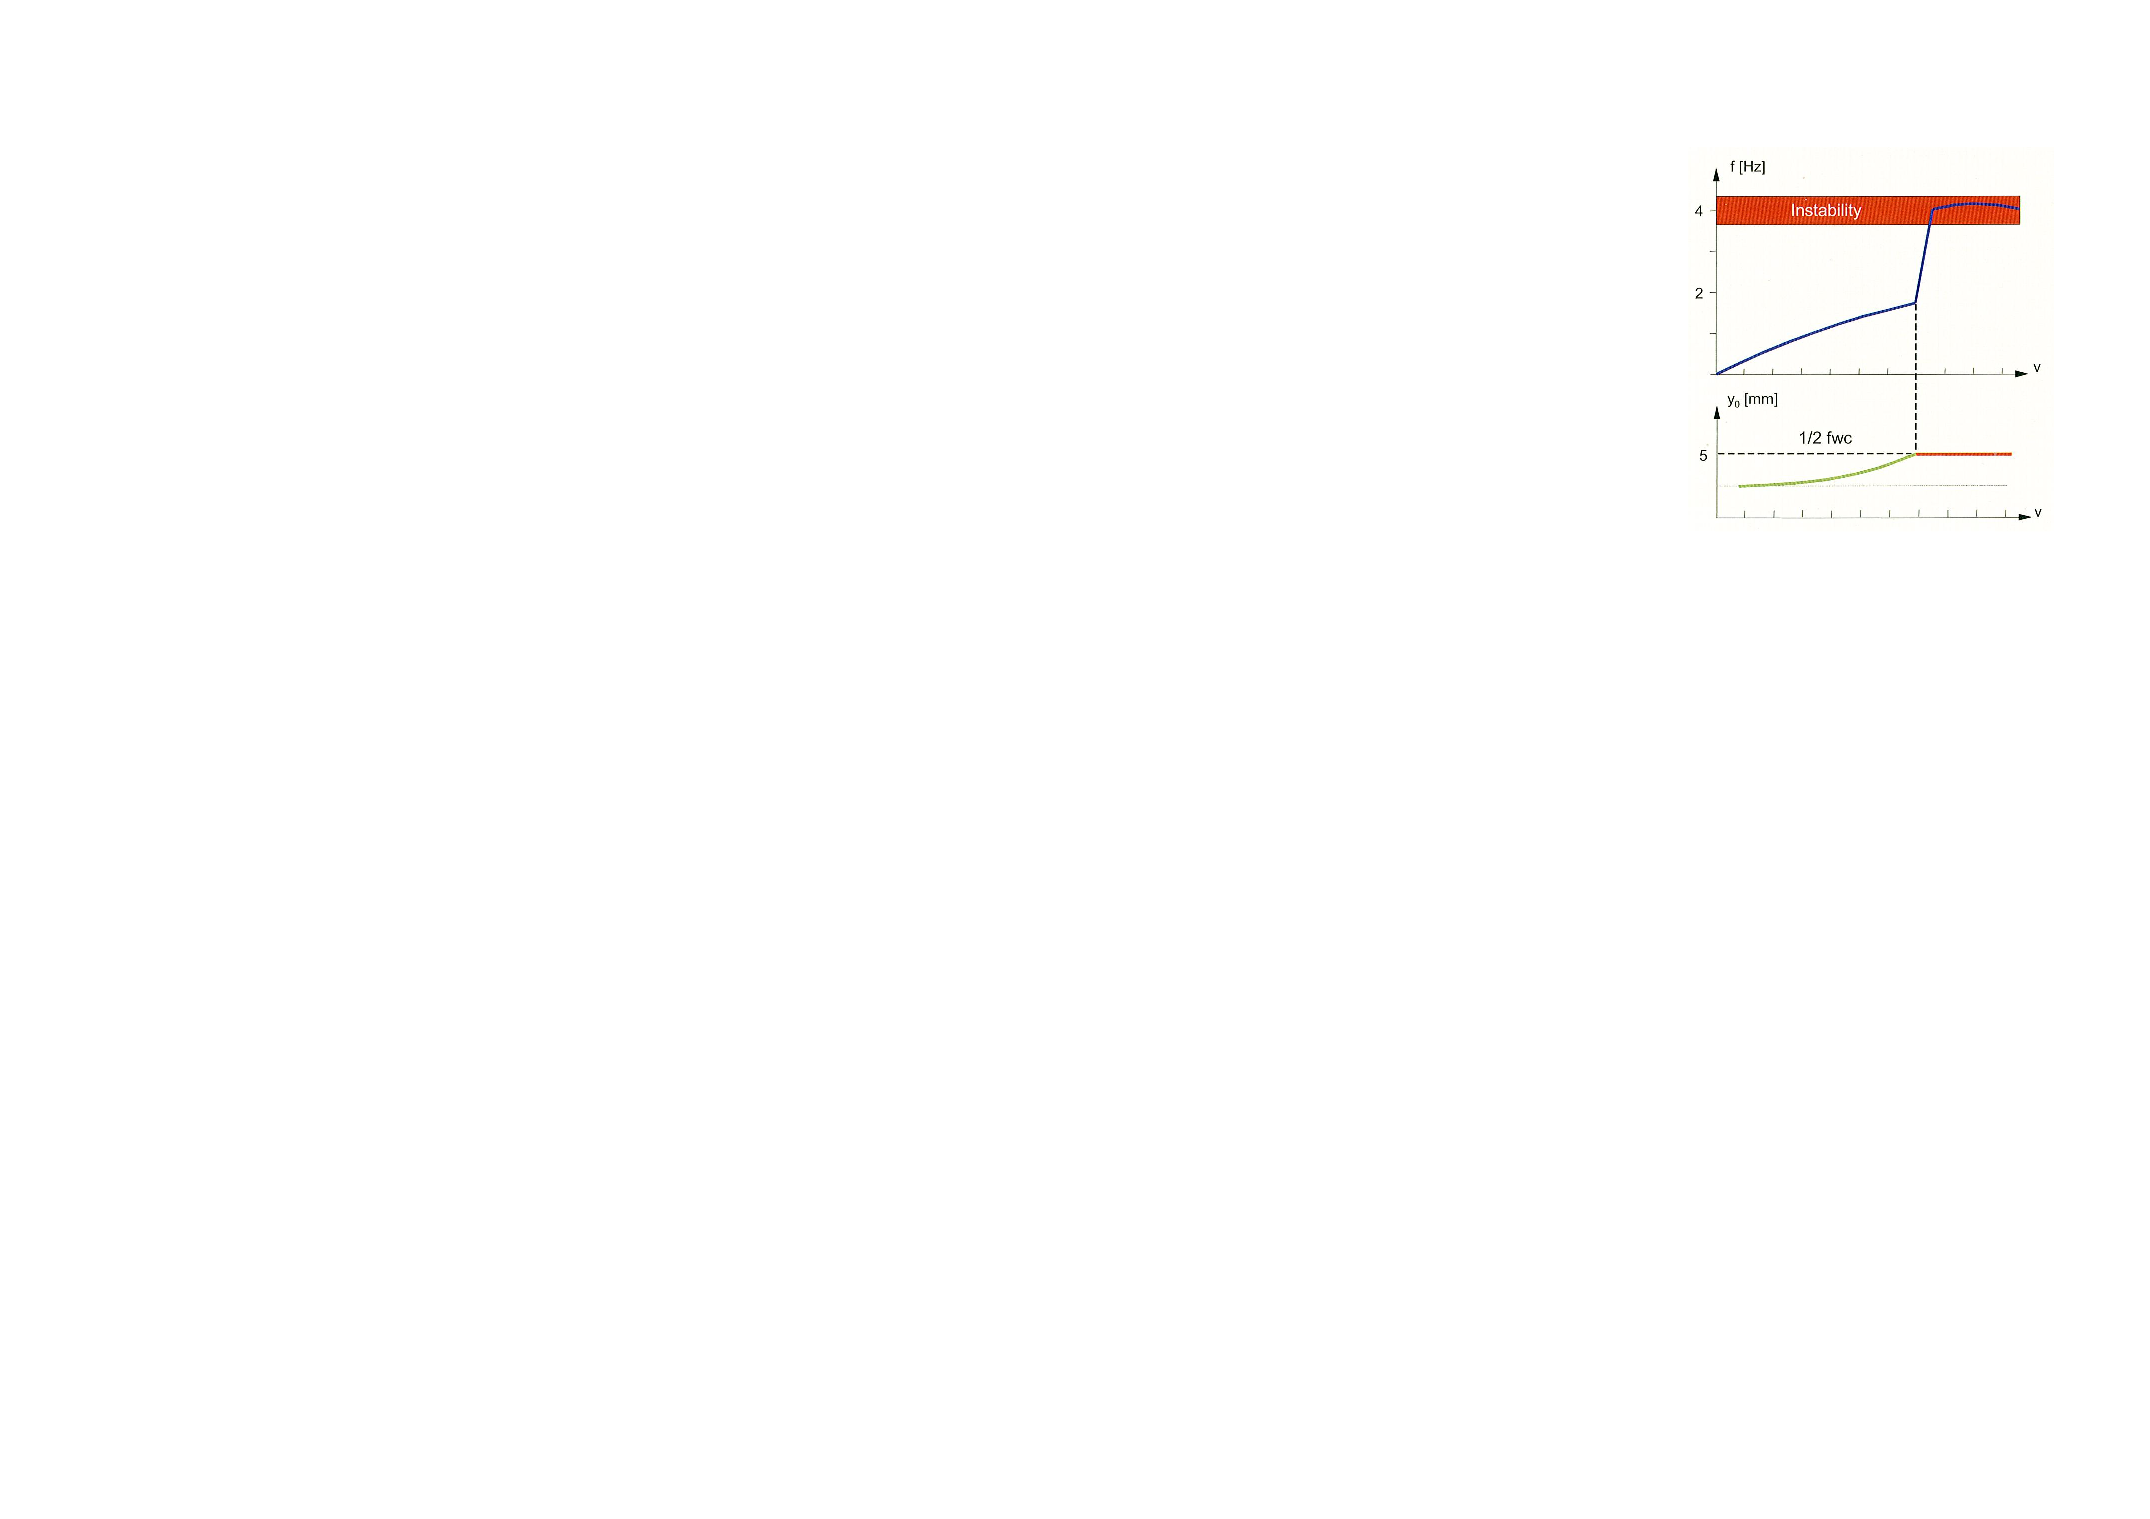
\includegraphics[width=0.5\textwidth]{amplitudefrequencyinstability}
	\caption{Increase in amplitude and frequency with speed and the development of instability. Extracted from \cite[Figure 2.6]{esveld2001modern}}
	\label{fig:amplitudefrequencystability}
\end{figure}

\section{Single and two-point contact between wheel and rail}
In the case of single-point contact, according to Figure, wheel load and lateral force act on the same point. This situation occurs when using worn wheel profiles. In the case of two-point contact, shown in Figure, the application points do not coincide.

Flanging occurs in the situation of double contact. 

\begin{figure}[h!]
\centering
	\begin{subfigure}[b]{0.2\textwidth}
    	\centering
    	
\includegraphics[width=\textwidth]{singlecontact}
    	\caption{Single contact point.  Extracted from \cite[Figure 2.13]{esveld2001modern}}
    	\label{fig:singlecontact}
	\end{subfigure}
	\begin{subfigure}[b]{0.5\textwidth}
    	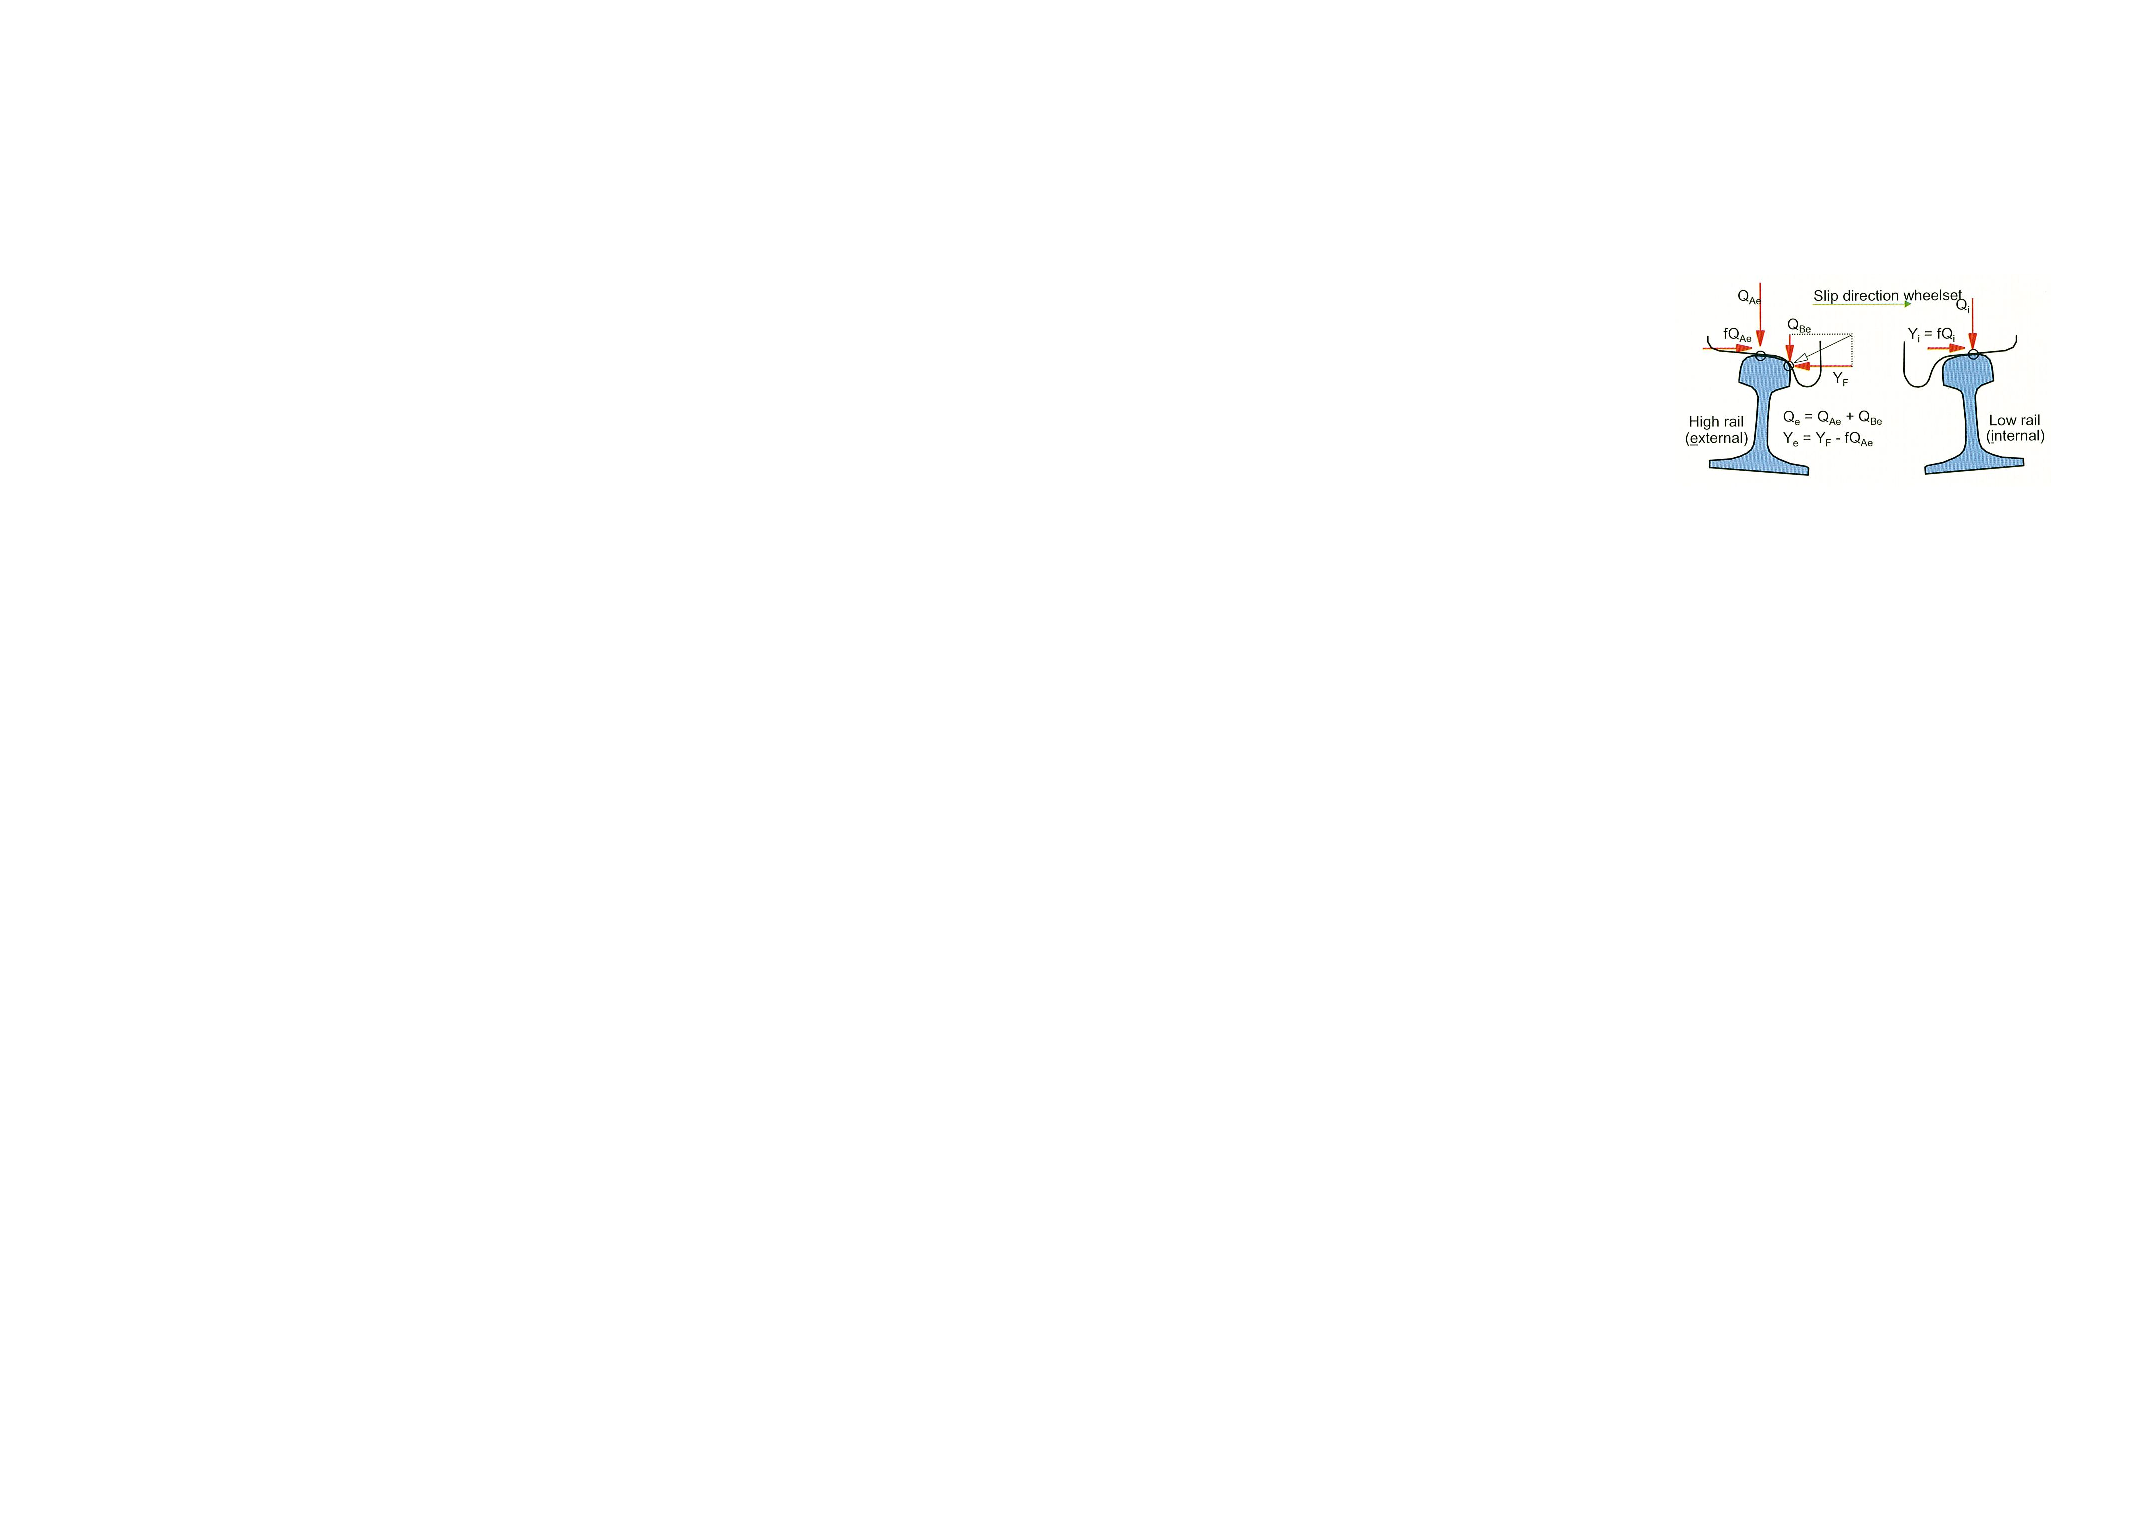
\includegraphics[width=\textwidth]{doublecontact}
    	\caption{Double contact point. Forces on rails in case of lateral slip in curves. Extracted from \cite[Figure 2.14]{esveld2001modern}}
    	\label{fig:doublecontract}
	\end{subfigure}
\end{figure}

\section{Dynamic theories}

\subsection{Natural frequencies and shapes of bridge}
Undamped Euler-Bernoulli beam theory is adopted to obtain natural wave shapes and frequencies of a bridge structure. This theory is the simplest bridge dynamic model which assumes that the bridge behaves as a vibrating uniform beam. 

The bridge is simply supported at both ends, and the stiffness is specified as a deflection at the mid span per unit span length arising from a static point load of 100kN at mid span.

The equation of vibration of a uniform beam is:

$$\frac{\partial^2 y}{\partial t^2} + a^2\frac{\partial^4 y}{\partial x^4}=0$$

where: 

y = deflection of beam

x = coordinates along longitudinal axis

t = time 

$a^2$ = EI/m

EI = flexural rigidity

and, m = mass per unit length

The general solution is:

$$y(x,t) = (A\cos pt+B\sin pt)(C\cos kx + D\sin kx + F\cosh kx + Gsinh kx)$$

which consists of independent time and distance parts. The distance dependent part of the solution gives the family of mode shapes which the beam will exhibit. Thus, generally, a beam has mode shapes which satisfy:

$$y(x) = C\cos kx + D\sin kx + F\cosh kx + Gsinh kx $$

For a beam which is simply supported at either end the general solution simplifies, giving a family of normalized amplitude mode shapes as follows:

$$y_r = \sin \frac{r\pi x}{L}$$

for $r = 1,2,3...,n$ and $L = span length$

with corresponding angular frequencies, $\omega_r$, of:

$$\omega_r = \frac{r^2 \pi^2}{L^2}\sqrt{\frac{EI}{m}}$$

thus natural frequencies $f_r$ of beam, are:

$$f_r = \frac{r^2 \pi}{2L^2}\sqrt{\frac{EI}{m}}$$

\subsection{Basic resonance concept}
The most simplest resonance scenario happens at a one degree-of-freedom mass-spring system loaded by a force whose frequency coincides with the natural frequency of mass-spring system.
\begin{figure}[h]
	\centering
	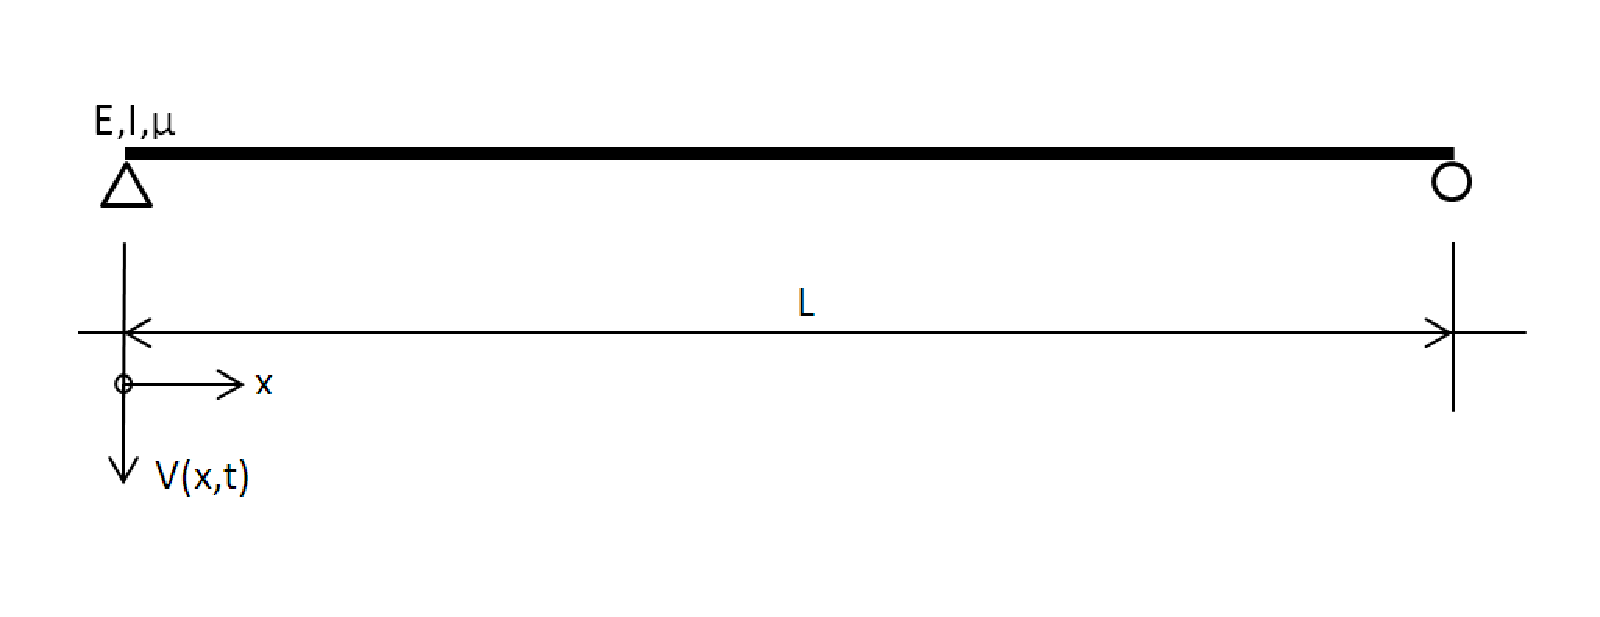
\includegraphics[width=0.8\textwidth]{massbeammodel.pdf}
	\caption{Mass beam model of span L}
	\label{fig:massbeammodel}
\end{figure}

Assume there is a simple one degree-of-freedom mass-spring system and an external force is acting on it. The force is given as $F(t)= F_0 \cos(\omega t)$. In this case the equation of motion takes the form
\begin{equation}
	m\ddot{x} + kx = F_0 \cos(\omega t)
\end{equation}

The general solution can be written as
\begin{equation}
	x(t) = A\cos(\omega_n t)+B\sin(\omega_n t) +\frac{F_0}{k}\frac{1}{1-\omega^2/\omega_n^2}\cos(\omega t)
\end{equation}

where $\omega_n = 2\pi\sqrt{k/m}$

The unknown constants A and B depend on the initial conditions.

The steady-state solution is given as:

\begin{equation}
	x_{steady}= X \cos(\omega t) = \frac{F_0}{k}\frac{1}{1-\omega^2/\omega_n^2}\cos(\omega t)
\end{equation}

The amplitude of vibrations of the mass-spring system is given by:
\begin{equation}
	|X|=|\frac{F_0}{k}\frac{1}{1-\omega^2/\omega_n^2}|
\end{equation}

The amplitude-frequency dependencies is shown in \ref{fig:amplitude-frequency-characteristic} 

\begin{figure}[h]
	\centering
	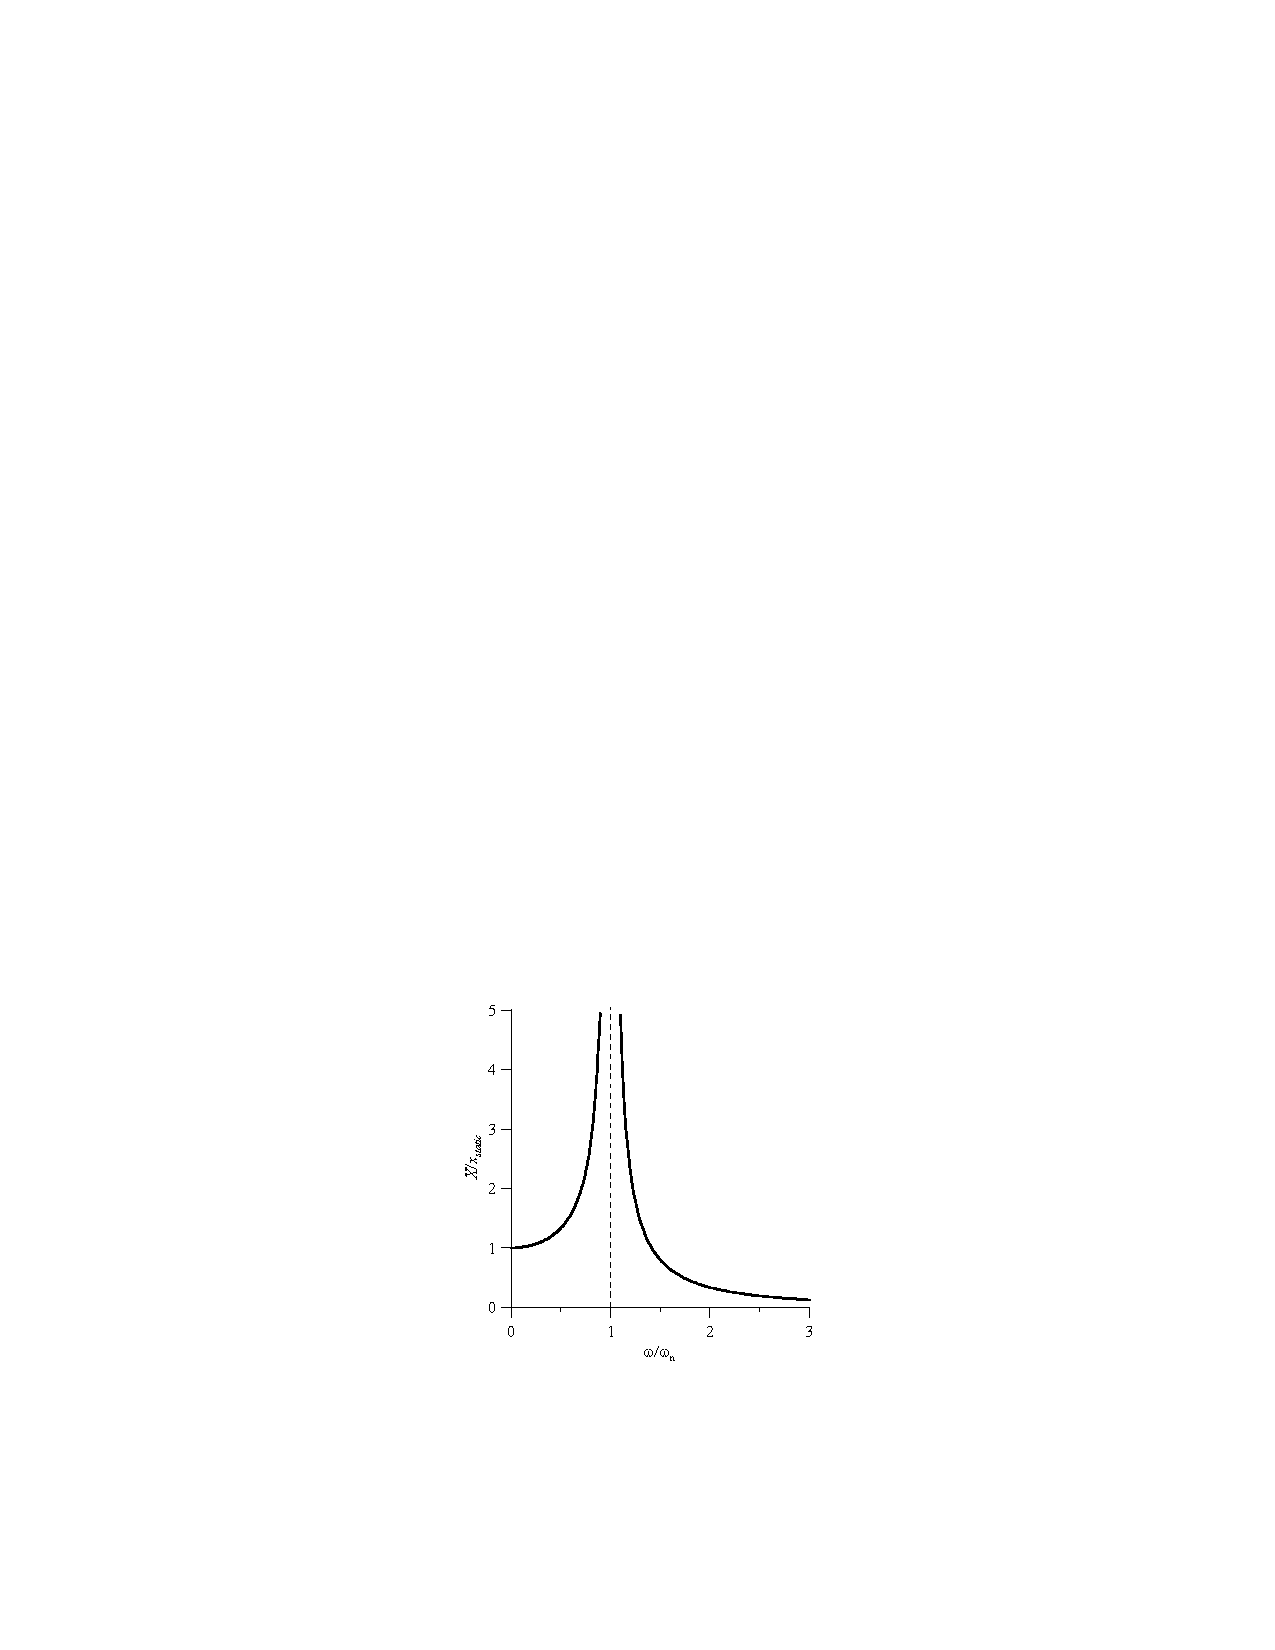
\includegraphics[width=0.6\textwidth]{amplitudefrequencycharacteristic.pdf}
	\caption{Amplitude-frequency characteristic. Extracted from \cite[2.2.2]{dynamicslecturenote}}
	\label{fig:amplitude-frequency-characteristic}
\end{figure}

When the frequency of force equals frequency of mass-spring system, the amplitude of vibration is infinitely high. It means system becomes unstable and normally it's a dangerous sign. This phenomenon is called resonance. Resonance can happen if the frequency of excitation coincides with the natural frequency of the excited systems.

Resonance can also happen when a harmonic force is loaded on an Euler-Bernoulli beam. It can be loaded anywhere on the beam to produce resonance. 

\subsection{Resonance between moving load and simplified beam bridge model}\label{sec:harmonicloadmodel}
It becomes a much more complicated problem when moving load is applied on an Euler-Bernoulli beam though analytical solution is still possible. Moving harmonic loads can represent, for instance, a component of the load transmitted to rails by moving trains. Thus it suits the aim of this thesis well.

\begin{figure}[h]
	\centering
	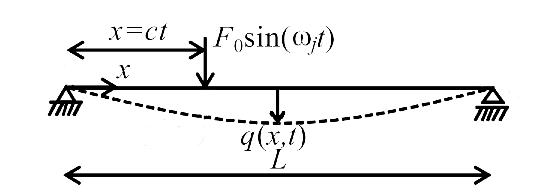
\includegraphics[width=0.5\textwidth]{harmonicloadbeam}
	\caption{Schematic representation of a generic beam crossed by a harmonic load}
	\label{fig:harmonicloadbeam}
\end{figure}

In most cases force input are hard to determine because of the complicity of wheel-rail interaction. But, in the context of lateral dynamics, the process can be simplified by adopting nosing forces. 

Giuseppe Piccoardo \cite{giuseppe2012dynamic} has provided following solutions:

The deflection $q(x,t)$ of a Euler-Bernoulli prismatic beam to a harmonic load moving with a constant speed $c$ (Figure\ref{fig:harmonicloadbeam}) is described by the well-known field equation

$$\mu \frac{\partial^2 q(x,t)}{\partial t^2} + \chi \frac{\partial q(x,t)}{\partial t}+EJ\frac{\partial^4 q(x,t)}{\partial x^4} = F_0 \sin(\Omega t)\delta(x-ct)[H(t)-H(t-L/c)]$$

where $\mu$ is the mass per unit length, $\chi$ is the damping coefficient, $EJ$ is the flexural stiffness, $F_0$ and $\Omega$ are, respectively, the amplitude and the circular frequency of the moving load, $\delta$ is the Dirac delta function, $H$ is the Heaviside step function, $L$ is the beam span length.

By using convolution integral, the solution can be expressed as:

\begin{equation}
	\label{eq:convolutionbefore}
	\begin{split}
		\tilde{p}(\tilde{t})=\varepsilon \exp (-\varepsilon \xi^* \tilde{t}) & \{ [\int_0^{\tilde{t}} \sin (\tilde{\Omega}\tilde{\tau})\phi_j(\varepsilon\Omega_c^* \tilde{\tau}) \exp (\xi^* \tilde{tau}) \cos(\tilde{\tau})]\sin(\tilde{t}) \\ 
		& -[\int_0^{\tilde{t}} \sin (\tilde{\Omega}\tilde{\tau})\phi_j(\varepsilon\Omega_c^* \tilde{\tau}) \exp (\xi^* \tilde{tau}) \cos(\tilde{\tau})]\cos(\tilde{t})\}
	\end{split}
\end{equation}

Under the hypothesis that $\tilde{\Omega} = 1$ (i.e., perfect resonance), Eq.\ref{eq:convolutionbefore} can be rewritten as follows

\begin{equation}
	\begin{split}
		\tilde{p}(\tilde{t})=\varepsilon \exp (-\varepsilon \xi^* \tilde{t}) & \{-[\frac{1}{2}\int_0^{\tilde{t}}\phi_j (\varepsilon \Omega_c^* \exp (\varepsilon \xi^* \tilde{tau}d\tilde{\tau}))]\cos (\tilde{t}) \\
		& +[\frac{1}{2}\int_0^{\tilde{t}}\sin(2\tilde{\tau})\phi_j (\varepsilon \Omega_c^* \exp (\varepsilon \xi^* \tilde{tau}d\tilde{\tau}))]\sin (\tilde{t}) \\
		& +[\frac{1}{2}\int_0^{\tilde{t}}\cos(2\tilde{\tau})\phi_j (\varepsilon \Omega_c^* \exp (\varepsilon \xi^* \tilde{tau}d\tilde{\tau}))]\cos (\tilde{t})\}
	\end{split}
\end{equation}

This equation can be solved numerically.


\section{FEM Modelling of rail-vehicle system}

\subsection{Modelling of railway vehicles}
According to Newton's law, 2 basic load effects are produced by moving train: vertical forces due to vehicle weight, and inertia effects caused by vehicle acceleration. The loads on a railway bridge are very complex problems thus in engineering practice, loads are often simplified. But, the simplification depends on the purpose of the analysis. 

\subsubsection{Moving vertical forces model}
If the inertia effects are neglected, loads of the moving trains can be modelled as moving vertical forces. For example, load diagram for type TALGO trains is shown in Figure.\ref{fig:verticalmodel} proposed by \cite{uic}.

\begin{figure}[h]
	\centering
	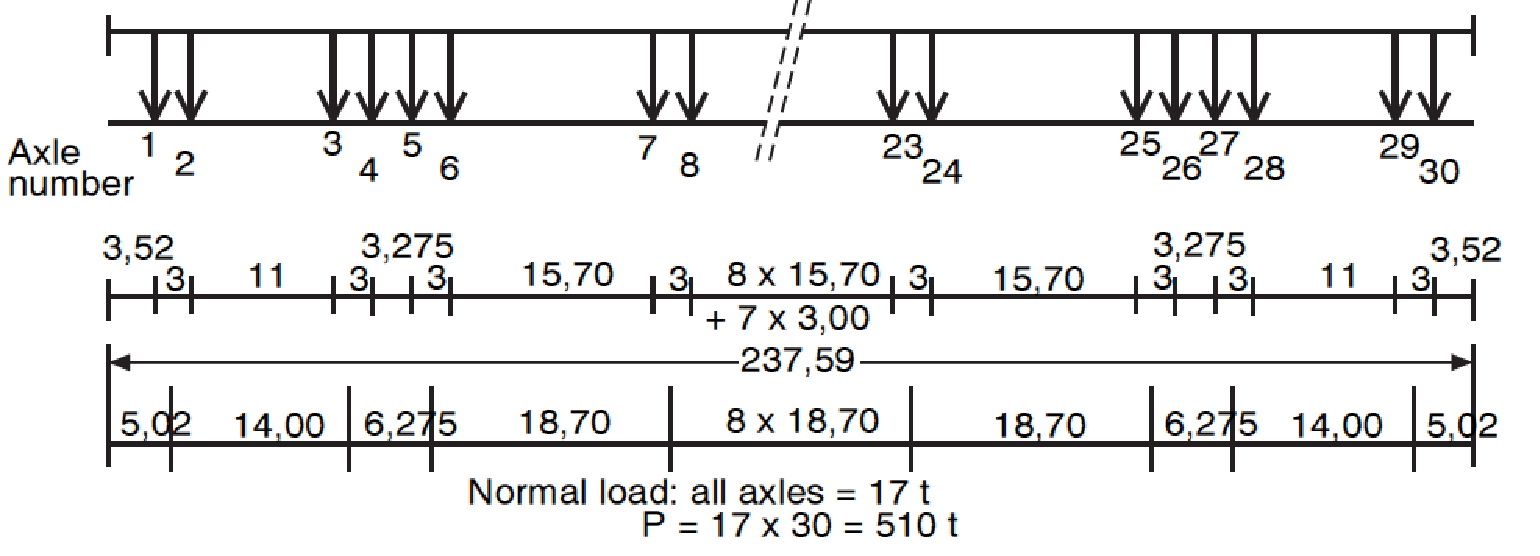
\includegraphics[width=0.8\textwidth]{verticalmodel.pdf}
	\caption{Moving vertical force model for TALGO trains}
	\label{fig:verticalmodel}
\end{figure}

\subsubsection{Advanced models}
Nowadays more and more models have been proposed to meet different requirements of railway bridge dynamic analysis. The complexity of these models differs from each other but they are all more complicated than moving vertical forces models. For example, vehicle-bridge interaction model takes vehicle suspension system into account, which gives an alternative for discovering resonance effects between bridge and the vehicle suspension systems. 

See Figure.\ref{fig:advancedmodel} for an example of advanced model.

\begin{figure}[p]
	\centering
	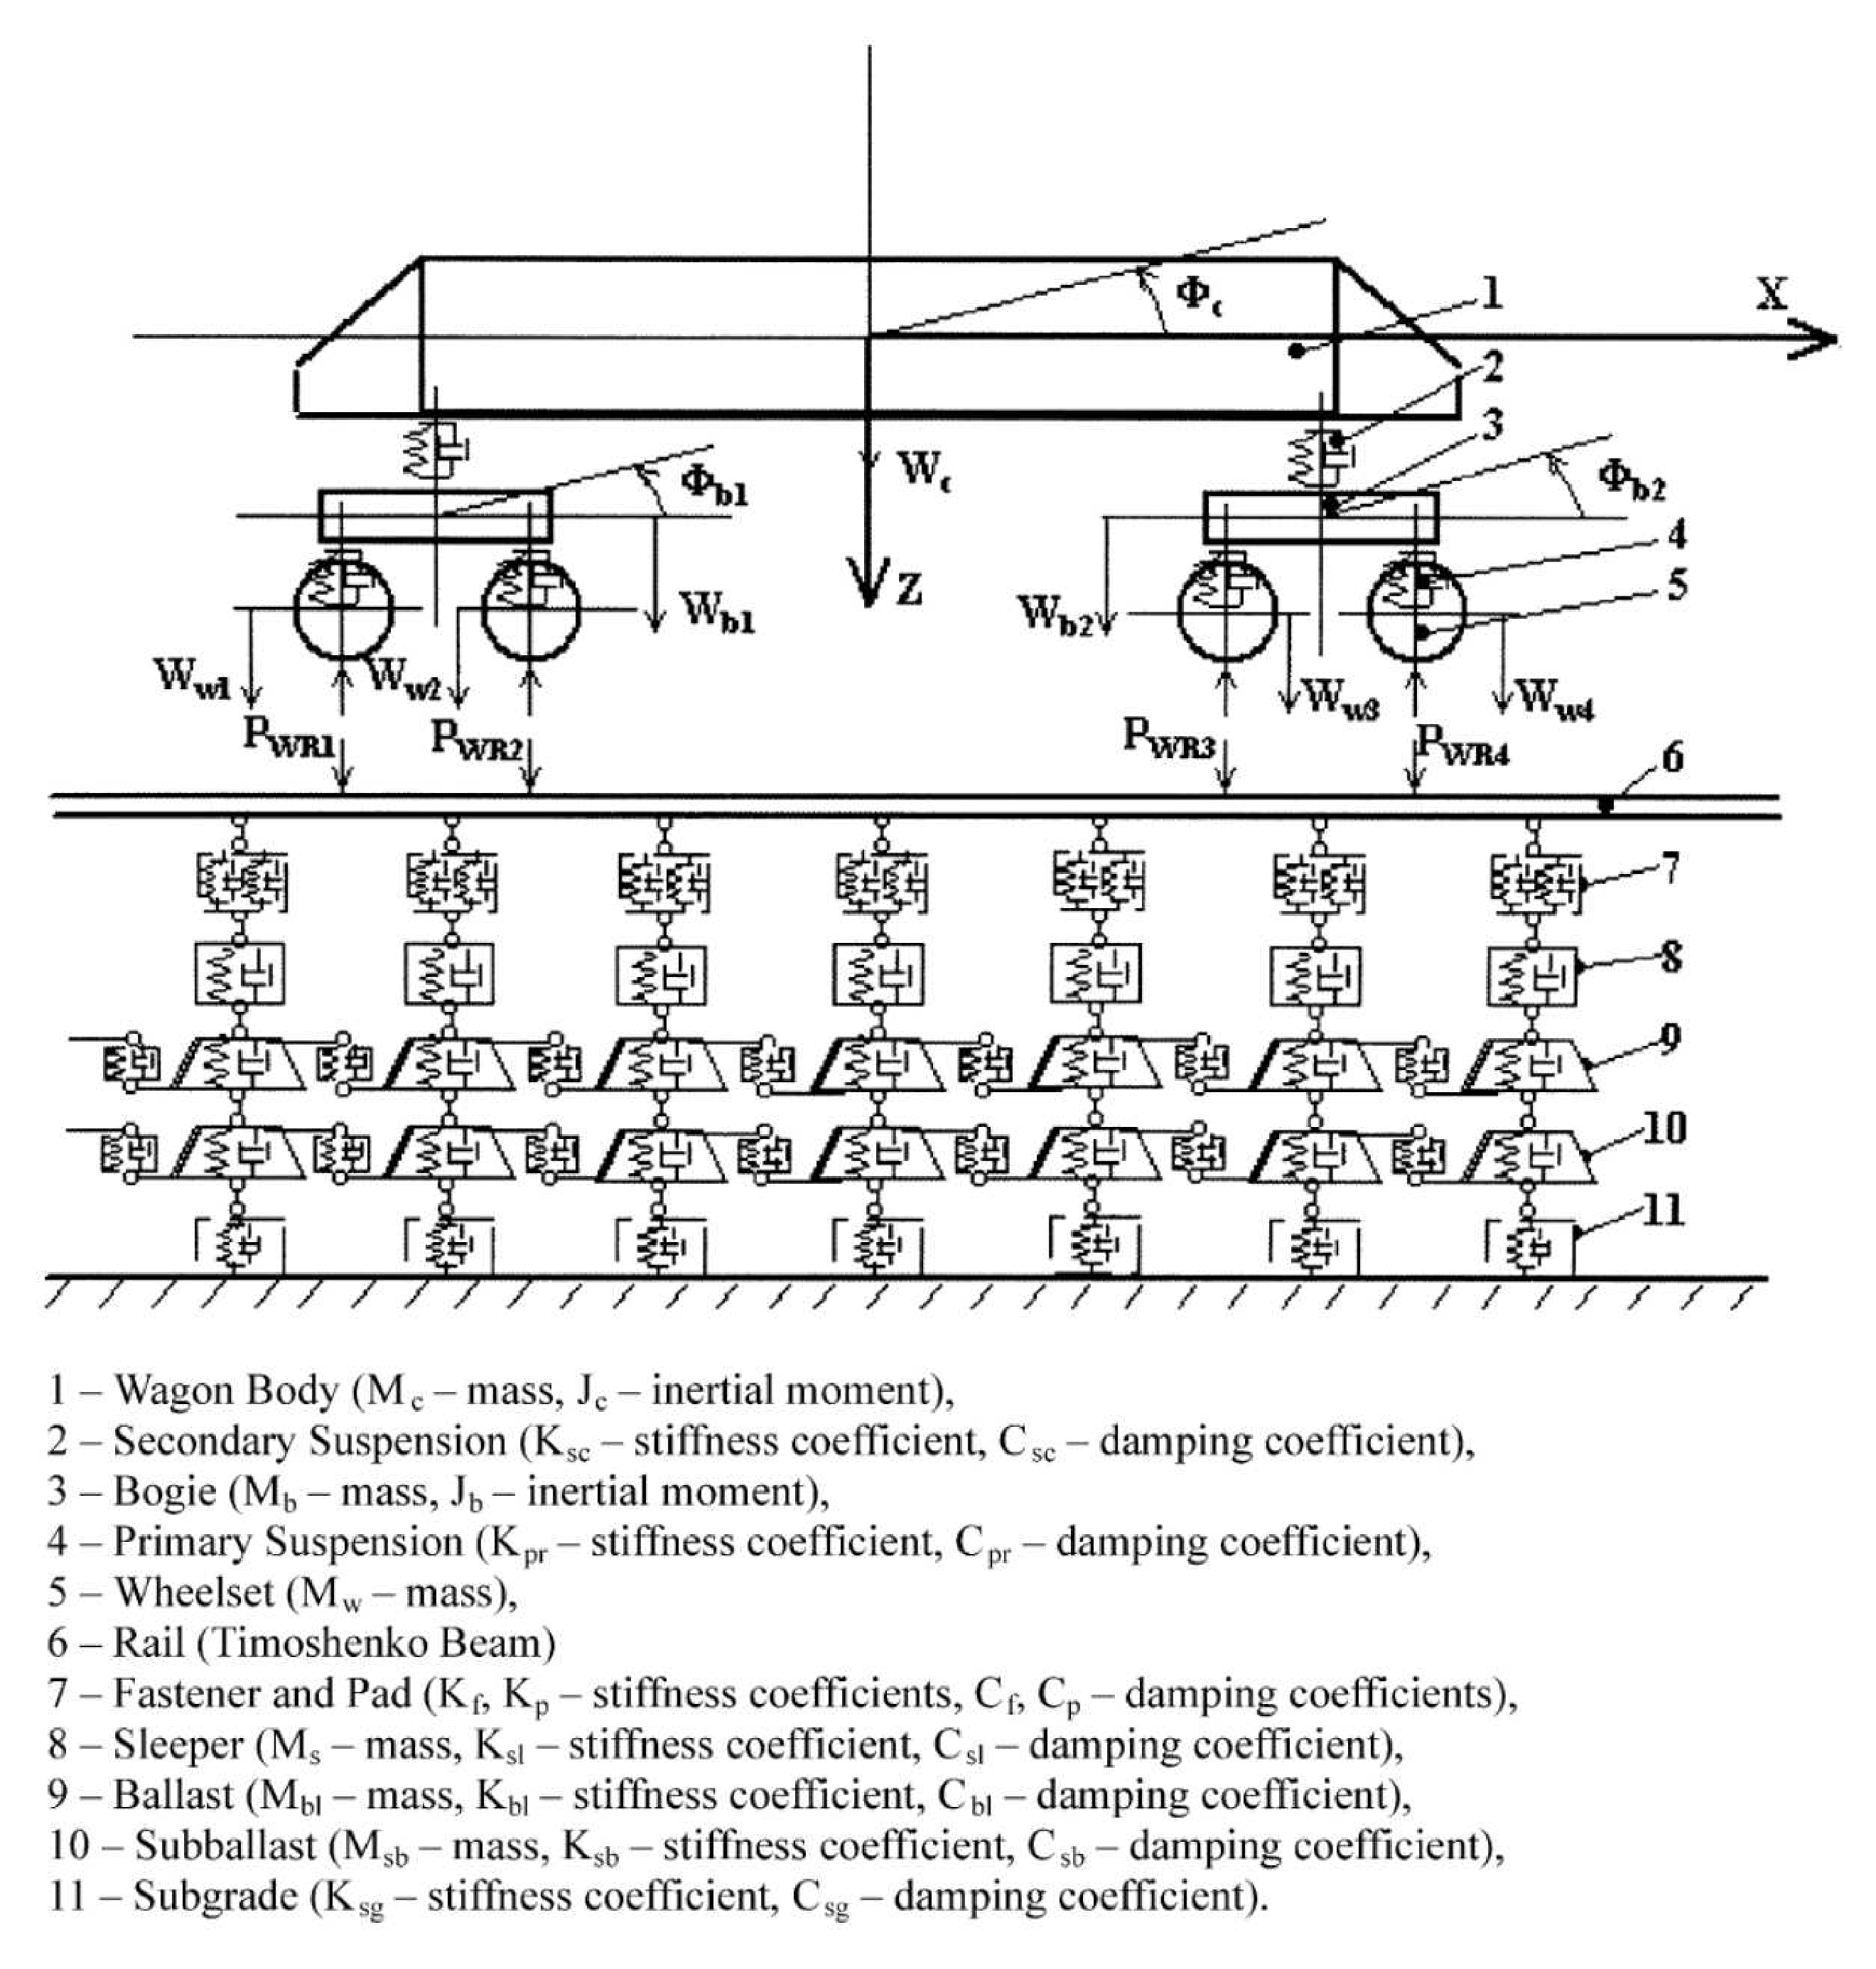
\includegraphics[width=0.8\textwidth]{advancedmodel.pdf}
	\caption{A dynamic model for the vertical interaction of the rail track and wagon system. Proposed in \cite{sun2002dynamic}}
	\label{fig:advancedmodel}
\end{figure}


\subsubsection{Models proposed in Eurocodes}

See Chapter~\ref{sec:train-models}

\subsection{Track model}
Proposed in \cite[A.6.1.3]{uic}, the track is represented by Timoshenko beam elements for the rails and takes account of the rail/sleeper fastening characteristics as well as the ballast(if one exists).

\textit{``A sleeper is generally represented by two beam elements, with two covering the rail and one used for the deck. Sleepers and ballast are modelled as concentrated masses. They are linked to the nodes of the rail and the bridge by a parallel spring and damper system. The track can be modelled to any length on both side of the bridges, where the stiffening effect of the bridge has to be taken into account. The effects of track distribution are not considered. Each vehicle is able to absorb the kinetic energy of the bridge and it is for this reason that, at resonance, the deflections and accelerations of the bridge obtained with this model are lower than those obtained with a live load diagram."}

The most complete model for analysing train/track/bridge interaction is shown in Figure

\begin{figure}[h]
	\centering
	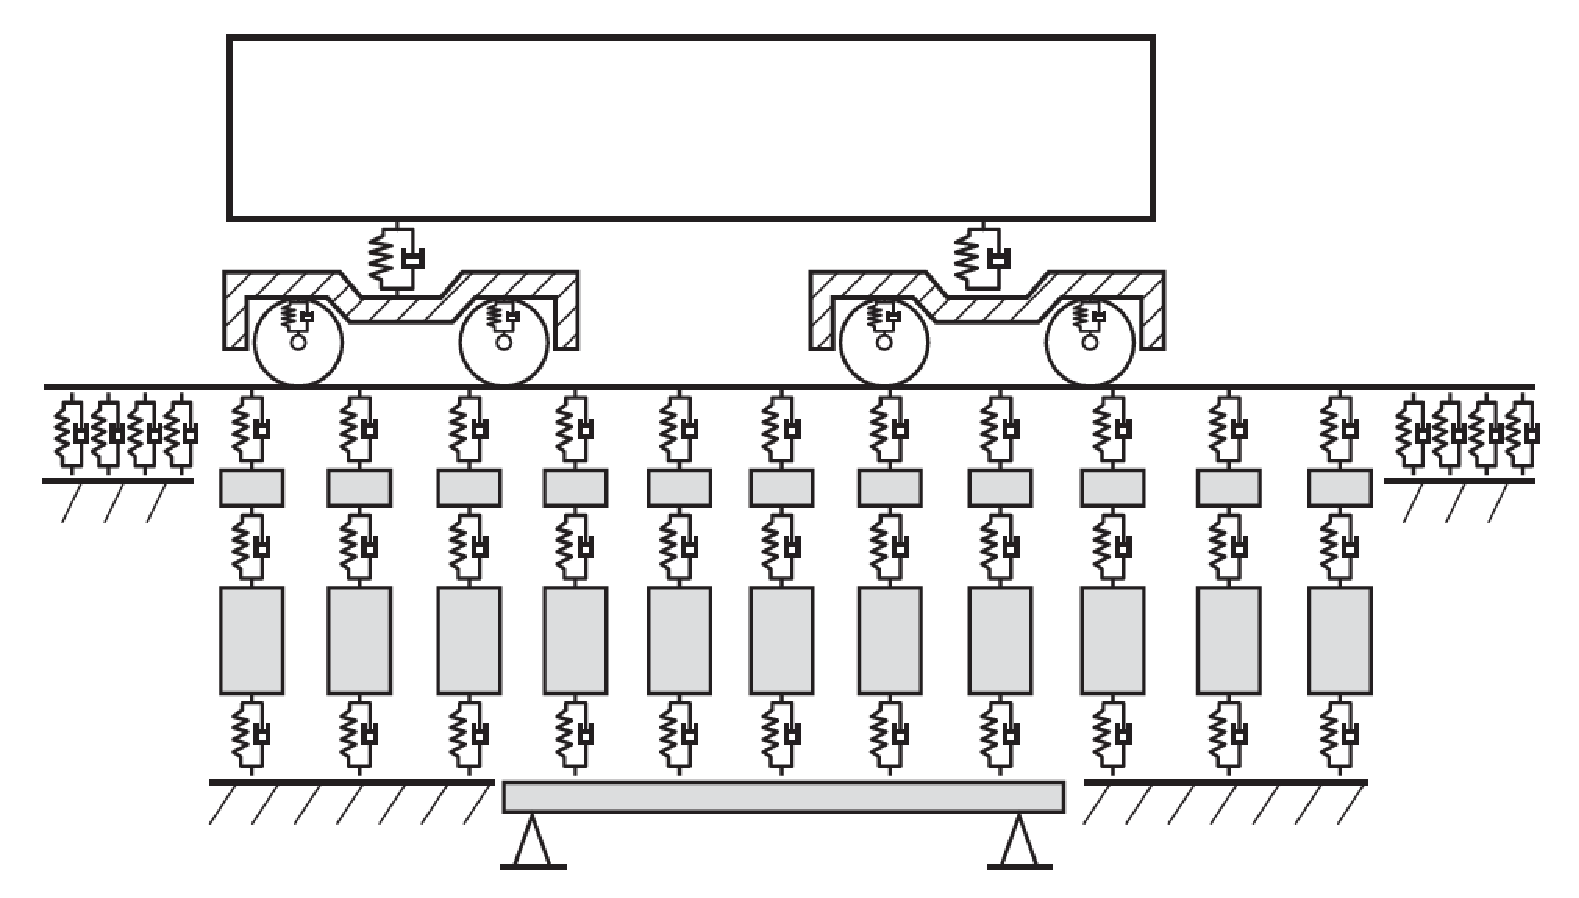
\includegraphics[width=0.8\textwidth]{trackmodel.pdf}
	\caption{Diagram of the dynamic train-track-bridge model. Extracted from \cite[Fig. 15]{uic}}
	\label{fig:trackmodel}
\end{figure}


\chapter{Literature Review of regulations regarding lateral railway bridge dynamics in 1991-2} 
Eurocode 1990 and Eurocode 1991-2 and their corresponding National Annex are primary codes to be fulfilled through out the whole process of conducting a railway bridge in Netherlands. It is of great importance to study dynamic effect on railway bridges due to increasing usage of public train service. What's more, as the need on capacity of railway service increase, high-speed train dynamic loading becomes a more general issue in the design of railway bridges. It is common knowledge that bridge structures loaded by high-speed trains have bigger chance of resonance, as well as of being required to be dynamic analysed in designing process. 

Unfortunately in Chapter 6.4 of Eurocode NEN-EN 1991-2-2003, the description of various subjects is vague including general procedures of conductinga dynamic analyses and methods of additional dynamic analysing calculating, etc. The following paragraphs aim to summarize Chapter 6.4 of Eurocode 1991-2 \cite{EC12}, in order to give a better interpretation. 

This literature research will be done by reviewing both physics knowledge and engineering standards.

% \section{Forced Vibrations under Harmonic Force}
% Assume there is a simple one degree-of-freedom mass-spring system and an external force is acting on it. The force is given as $F(t)= F_0 \cos(\omega t)$. In this case the equation of motion takes the form
% \begin{equation}
% 	m\ddot{x} + kx = F_0 \cos(\omega t)
% \end{equation}

% The general solution can be written as
% \begin{equation}
% 	x(t) = A\cos(\omega_n t)+B\sin(\omega_n t) +\frac{F_0}{k}\frac{1}{1-\omega^2/\omega_n^2}\cos(\omega t)
% \end{equation}

% The unknown constants A and B depend on the initial conditions.

% The steady-state solution is given as:

% \begin{equation}
% 	x_{steady}= X \cos(\omega t) = \frac{F_0}{k}\frac{1}{1-\omega^2/\omega_n^2}\cos(\omega t)
% \end{equation}

% The amplitude of vibrations of the mass-spring system is given by:
% \begin{equation}
% 	|X|=|\frac{F_0}{k}\frac{1}{1-\omega^2/\omega_n^2}|
% \end{equation}

% The amplitude-frequency dependencies is shown in \ref{fig:amplitude-frequency-characteristic} 

% \begin{figure}[h]
% 	\centering
% 	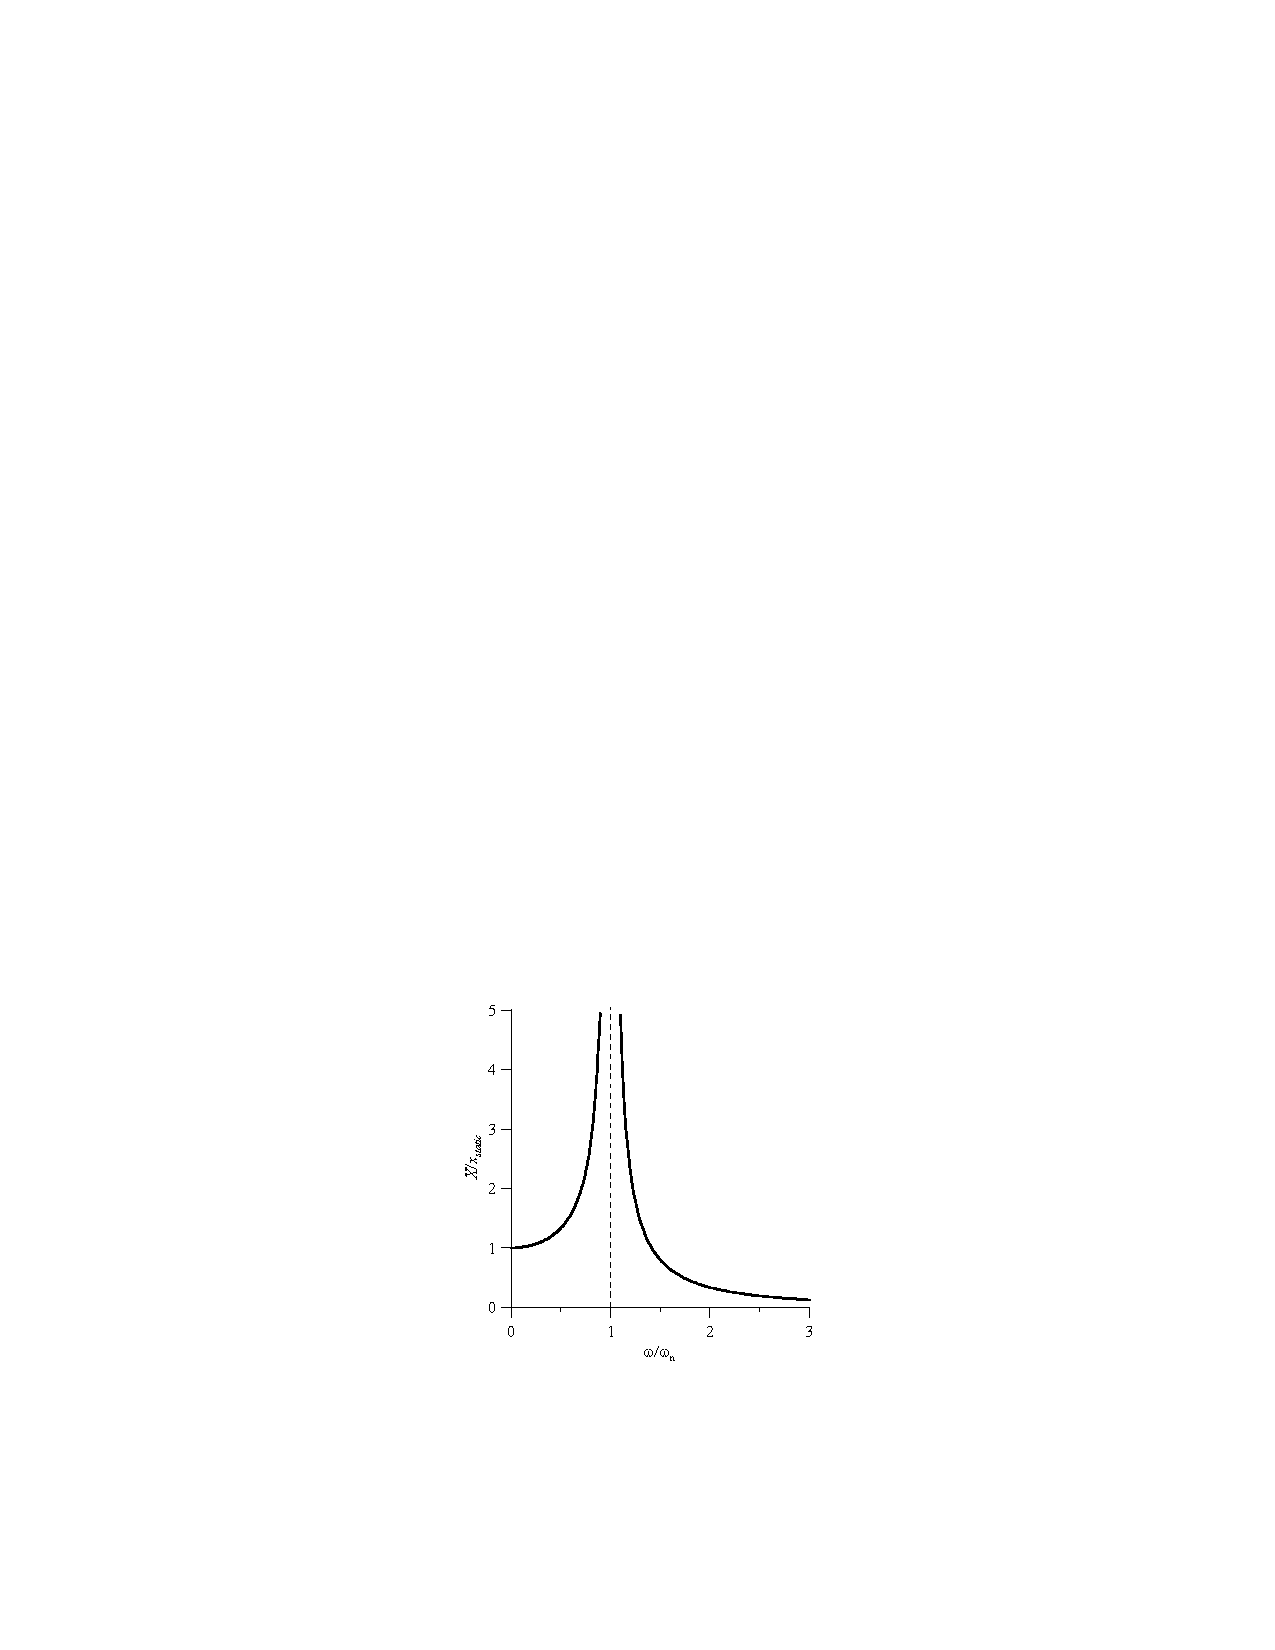
\includegraphics[width=0.6\textwidth]{amplitudefrequencycharacteristic.pdf}
% 	\caption{Amplitude-frequency characteristic. Extracted from \cite[2.2.2]{dynamicslecturenote}}
% 	\label{fig:amplitude-frequency-characteristic}
% \end{figure}


% \section{Introduction to the dynamics of railway bridges}

% \cite{fryba1996dynamics}Dynamics of railway bridges is concerned with the study of deflections and stresses in railway bridges. The loads are represented by the moving wheel and axle forces, by means of which railway vehicles transmit their load and inertia actions to railway bridges. A survey of the dynamic effects of vehicles on railway bridges is given in Figure.\ref{fig:dynamic effects}

% \begin{figure}[h]
% 	\centering
% 	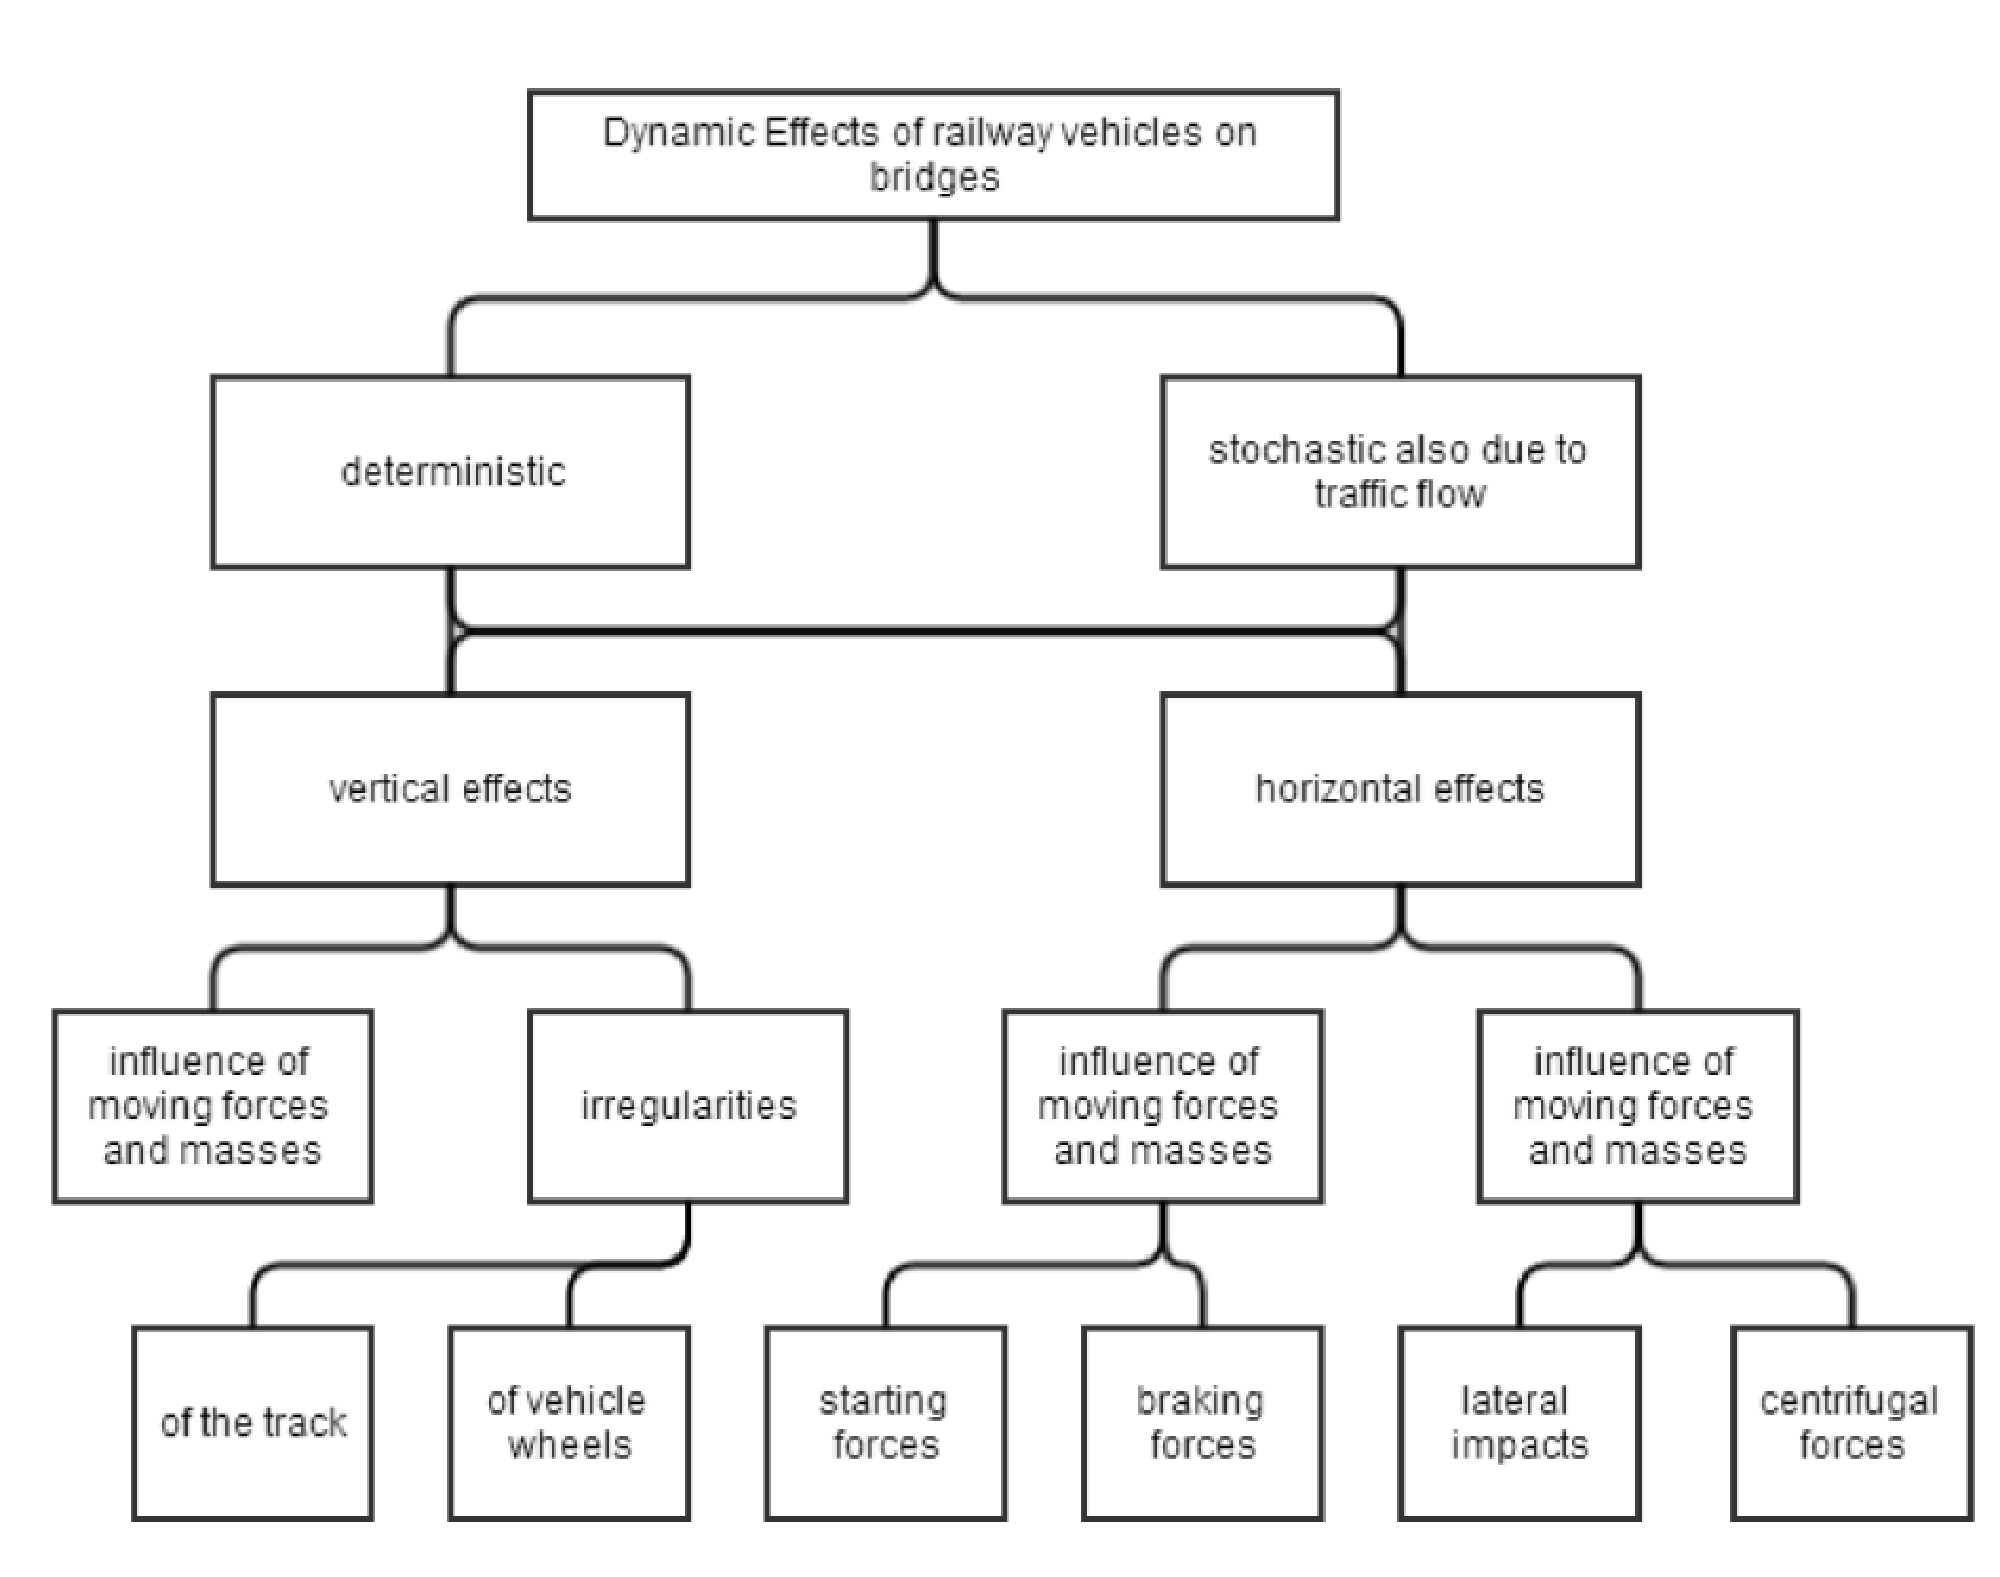
\includegraphics[width=0.6\textwidth]{dynamiceffects.pdf}
% 	\caption{Dynamic effects of railway vehicles on bridges. Extracted from \cite[1.1]{fryba1996dynamics} }
% 	\label{fig:dynamic effects}
% \end{figure}

\section{Factors influencing dynamic behaviour}
As stated in\cite[6.4.2]{EC12} there are 11 factors influencing dynamic behaviour of a railway bridge. The principal factors which influence dynamic behaviour are:
\begin{enumerate}[-]
	\item the speed of traffic across the bridge
	\item the span L of the element and the influence line length for deflection of the element being considered
	\item the mass of the structure
	\item the natural frequencies of the whole structure and relevant elements of the structure and the associated mode shapes (eigenforms) along the line of the track
	\item the number of axles, axle loads and the spacing of axles
	\item the damping of the structure
	\item vertical irregularities in the track
	\item the unsprung/sprung mass and suspension characteristics of the vehicle
	\item the presence of regularly spaced supports of the deck slab and/or track (cross girders, sleepers etc.)
	\item vehicle imperfections (wheel flats, out of round wheels, suspension defects etc.)
	\item the dynamic characteristics of the track (ballast, sleepers, track components etc.)
\end{enumerate}

Other factors may include:

\begin{enumerate}

	\item The track number of the bridge and their alignment. 
	\item Multiple trains running on bridge simultaneously. 
	\item Track alignment

\end{enumerate}

\section{Requirements for railway bridge verification}
\cite{EC0} propose following requirements


\begin{enumerate}
	\item Checks on bridge deformations shall be performed for traffic safety purposes for the following items:
	\begin{enumerate}[-]
		\item vertical accelerations of the deck
		\item vertical deflection of the deck throughout each span
		\item unrestrained uplift at the bearings(to avoid premature bearing failure)
		\item vertical deflection of the end of the deck beyond bearings(to avoid destabilising the track, limit uplift forces on rail fastening systems and limit additional rail stresses) 
		\item twist of the deck measured along the centre line of each track on the approaches to a bridge and across a bridge(to minimise the risk of train derailment)
		\item rotation of the ends of each deck about a transverse axis or the relative total rotation between adjacent deck ends(to limit additional rail stresses, limit uplift forces on rail fastening systems and limit angular discontinuity at expansion devices and switch blades)
		\item longitudinal displacement of the end of the upper surface of the deck due to longitudinal displacement and rotation of the deck end(to limit additional rail stresses and minimise disturbance to track ballast and adjacent track formation)
		\item \textbf{horizontal transverse deflection(to ensure acceptable horizontal track radii)}
		\item \textbf{horizontal rotation of a deck about a vertical axis at ends of a deck (to ensure acceptable horizontal track geometry and passenger comfort)}
		\item \textbf{limits on the first natural frequency of lateral vibration of the span to avoid the occurrence of resonance between the lateral motion of vehicles on their suspension and the bridge}
	\end{enumerate}
	\item Checks on bridge deformations should be performed for passenger comfort, i.e. vertical deflection of the deck to limit coach body acceleration in accordance with A2.4.4.3\cite{EC0}
	\item The limits given in A2.4.4.2 and A2.4.4.3\cite{EC0} take into account the mitigating effects of track maintenance (for example to overcome the effects of the settlement of foundations, creep, etc.) 
\end{enumerate}


% \section{Vertical Dynamic effects}
% As stated in EN 1991-2\cite{EC12}, the static stress and deformations (and associated bridge deck acceleration) induced in a bridge are increased and decreased under the effects of moving traffic by the following:

% \begin{enumerate}[-]
% 	\item the rapid rate of loading due to the speed of traffic crossing the structure and the inertial response (impact) of the structure,
% 	\item the passage of successive loads with approximately uniform spacing which can excite the structure and under certain circumstances create resonance (where the frequency excitation(or a multiple there of) matches a natural frequency of the structure (or a multiple there of), there is a possibility that the vibrations caused by successive axles running onto the structure will be excessive),
% 	\item variations in wheel loads resulting from track or vehicle imperfections (including wheel irregulations).
% \end{enumerate}
% For determining the effects (stresses, deflections, bridge deck acceleration etc.) of rail traffic actions the above effects shall be taken into account.


% \subsection{Train Actions}
% See section \ref{designprocedures}


% \subsection{Wind Actions}
% The nature of the wind load is dynamic. This means that its magnitude varies with respect to time and space.

% According to \cite{mohammadi2013wind}: The limitations behind the applications of the EN-1991-1-4, Eurocode1, actions on structures-general actions-wind load-part 1-4, lead the structural designers to a great confusion. This may be due to the fact that, EC1 provides only the guid- ance for the bridges whose fundamental mode of vibrations have constant sign (e.g. simply supported structures) or a simple linear sign (e.g. cantilever structures) and these modes are the governing mode of vibrations of the structure; it analyzes only the along-wind response of the structure and not the cross wind response and the simplified methods recommended in this code are covering only the structures with simple geometrical configurations.

\section{Horizontal transverse dynamic effects}
There's only one criterion in the Eurocodes mentioned that the bridge's first lateral natural frequency should no lower that 1.2 Hz. 

However, as more and more long-span bridges are built nowadays, this requirement is not valid for more bridges. This is because, in general, the lateral natural frequency of a bridge decreases when span increases. For bridges with span longer than 100m, there's few bridge can have a lateral frequency higher than 1.2Hz, according to senior engineers' designing experience.

So it is vital to discuss horizontal dynamic effects for the sake of longer span bridges. In additional, study the requirements for horizontal vibration of railway bridges to make the results of dynamic analysis usable.



% \subsection{Horizontal vibration of a beam}

% Fryba\cite{fryba1996dynamics} described the first two sources in mathematical terms:
% Consider a simply supported beam loaded by moving train loading, horizontal vibrations of the beam in a transverse direction $ w(x,t) $ are generated by lateral random forces $ H_n (t) $ due to random irregularities and sinusoidal motion. The differential equation for the deformation is:

% \begin{equation}
% 	EI_yw^{IV}(w,t)+\mu \ddot{w} (x,t)=\sum_{n=1}^{N} \varepsilon_n\delta(x+d_n-ct)H_n(t) 
% \end{equation}

% where $ H_n(t) $ stands for forces due to random irregularities and sinusoidal motion. $ H_n(t) $ is of a typically random character and can be replaced by horizontal transverse forces with zero mean values. See Figure.~\ref{fig:trackirrg} for example.

% \cite[Table 9.1]{fryba1996dynamics} gives sample of natural frequencies of steel truss bridges with open deck. Shown as follow Table~\ref{tab:spatialvibrationsteel}. Please note that truss bridges have high stiffness.

% \begin{table}[h]
% 	\centering
% 	\begin{tabular}{ccccc}
% 		\hline
% 		\multirow{2}{*}{Vibration Type} & \multirow{2}{*}{Symbol} & \multirow{2}{*}{j} & \multicolumn{2}{c}{Bridge with span} \\
% 		\cline{4-5}
% 		 & & & $ l=25.85m $ & $ l=48.4m $\\
% 		\hline
% 		\multirow{3}{*}{Vertical} & \multirow{3}{*}{$ f_j $} & 1 & 8.7 & 5.4\\
% 		 & & 2 & 34.7 & 21.5 \\
% 	 	 & & 3 & 78.1 & 48.3 \\
% 	 	\hline
% 	 	\multirow{9}{*}{Horizontal} & \multirow{3}{*}{$ f_{hj} $} & 1 & 15.3 & 4.7 \\
% 	 	 & & 2 & 61.1 & 19.0 \\
% 	 	 & & 3 & 137.5 & 42.7 \\
% 	 	\cline{2-5}
% 	 	 & \multirow{3}{*}{$ f_{yj} $} & 1 & 14.8 & 4.7 \\
% 	 	 & & 2 & 53.9 & 18.1 \\
% 	 	 & & 3 & 107.4 & 38.8 \\ 
% 	 	\cline{2-5}
% 	 	 & \multirow{3}{*}{$ {f}'_{yj} $} & 1 & 14.7 & 4.6 \\
% 	 	 & & 2 & 52.5 & 17.5 \\
% 	 	 & & 3 & 101.7 & 36.4 \\ 
% 	 	\cline{2-5}
% 	 	\hline
% 	 	\multirow{9}{*}{Torsional} & \multirow{3}{*}{$ f_{\xi j} $} & 1 & 35.7 & 19.2 \\
% 	 	 & & 2 & 71.3 & 38.4 \\
% 	 	 & & 3 & 107.0 & 57.7 \\
% 	 	\cline{2-5}
% 	 	 & \multirow{3}{*}{$ f_{\varphi j} $} & 1 & 34.9 & 16.7 \\
% 	 	 & & 2 & 73.5 & 35.4 \\
% 	 	 & & 3 & 117.4 & 56.9 \\ 
% 	 	\cline{2-5}
% 	 	 & \multirow{3}{*}{$ {f}'_{\varphi j} $} & 1 & 36.5 & 19.7 \\
% 	 	 & & 2 & 77.6 & 41.9 \\
% 	 	 & & 3 & 126.4 & 67.5 \\ 
% 	 	\hline
% 	\end{tabular}
% 	\caption{Spatial vibrations of steel truss bridges with open bridge deck}
% 	\label{tab:spatialvibrationsteel}
% \end{table}


% \begin{figure}[p]
% 	\centering
% 	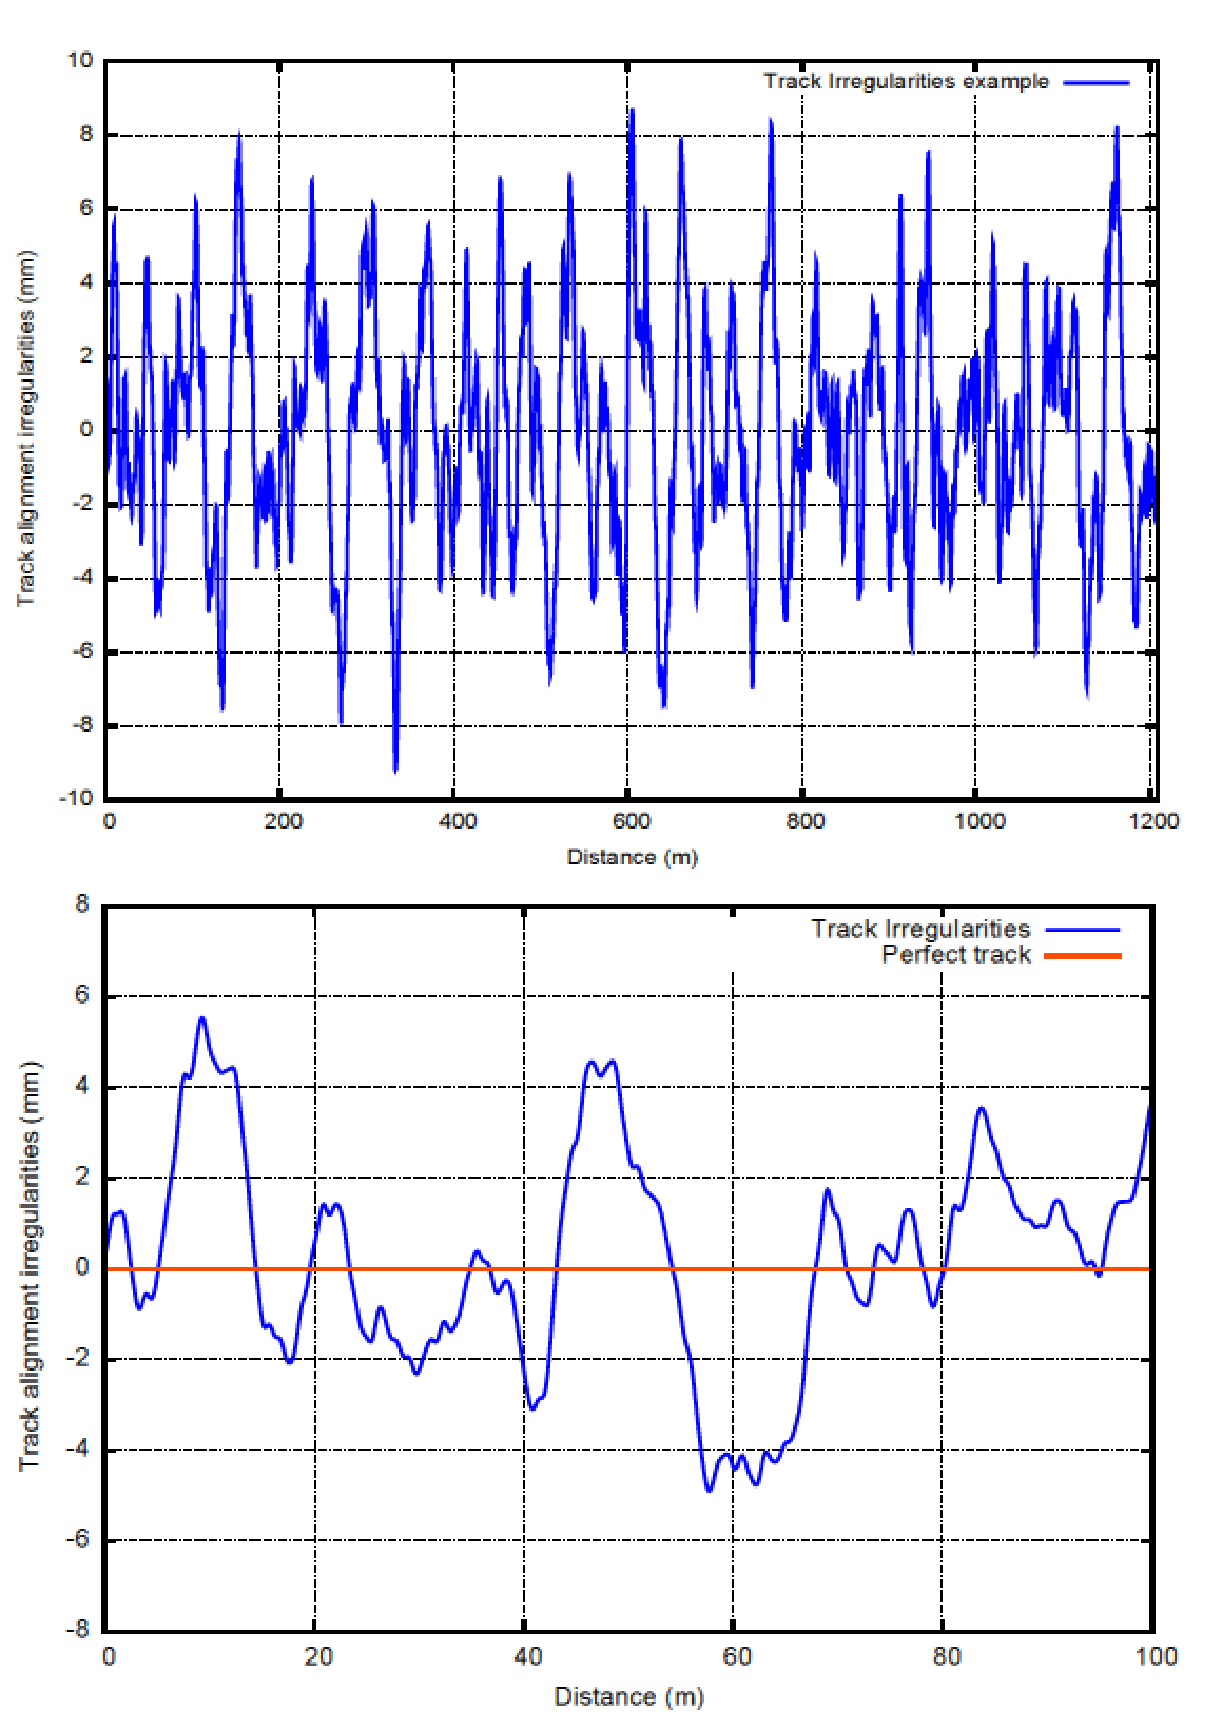
\includegraphics[width=0.8\textwidth]{trackirregularities.pdf}
% 	\caption{Example of a track lateral alignment irregularities profile for a track with low irregularities in a total length of 1209m.  Extracted from \cite{da2007dynamic}}
% 	\label{fig:trackirrg}
% \end{figure}


% \subsubsection{Centrifugal forces}
% In \cite[6.5.1]{EC12} specifies following principles about centrifugal forces act on railway bridges:

% Where the track on a bridge is curved over the whole or part of the length of the bridge, the centrifugal force and the track cant shall be taken into account.

% The centrifugal forces should be taken to act outwards in a horizontal direction at a height of 1.80m above the running surface (see \cite[Figure 1.1]{EC12}). For some traffic types, e.g. double stacked containers, an increased value of $h_t$ should be specified.

% The centrifugal force shall always be combined with the vertical load. The centrifugal force shall not be multiplied by the dynamic factor $\varPhi_1$ or $\varPhi_3$.

% The characteristic value of the centrifugal force shall be determined according to the following equations:

% \begin{equation}
% 	Q_tk=\frac{v^2}{g \cdot r}(f \cdot Q_{vk})=\frac{V^2}{127r}(f \cdot Q_{vk})
% \end{equation}

% \begin{equation}
% 	q_{tk}=\frac{v^2}{g \cdot r}(f \cdot q_{vk})=\frac{V^2}{127r}(f \cdot q_{vk})
% \end{equation}

% where:

% \begin{tabular}{ll}
% $Q_{tk}$,$q_{tk}$ & Characteristic values of the centrifugal forces\\
% $Q_{vk}$,$q_{vk}$ & Characteristic values of the vertical loads specified in \cite[6.3]{EC12}\\
% $f$ & Reduction factor, see below \\
% $v$ & Maximum speed in accordance with \cite[6.5.1(5)]{EC12}[m/s]\\
% $V$ & Maximum speed in accordance with \cite[6.5.1(5)]{EC12}[km/h]\\
% $g$ & Acceleration due to gravity [9.81$m/s^2$]\\
% $r$ & Radius of curvature [m].
% \end{tabular}

% For Load Model 71 (and where required Load Model SW/0) the reduction factor $f$ is given by:

% \begin{equation}
% 	f=[1-\frac{V-120}{1000}(\frac{814}{V}+1.75)(1-\sqrt{\frac{2.88}{L_f}})]
% \end{equation}

 

% \section{Torsional vibration}
% According to \cite[9.1.3]{fryba1996dynamics}, the horizontal lateral forces of railway vehicles act on the rial top level,i.e. outside the cross section centroid of the bridge in the majority of cases. Let the difference of elevations be $ h $. Consequently, they affect the bridge by twisting moments $ hH_n(t) $. The differential equation of a beam due to simple torsion is 
% \begin{equation}
% 	-GI_\xi \xi''(x,t)+\mu \ddot{\xi}(x,t)=\sum_{n=1}^{N}\varepsilon_n \delta (x+d_n-ct)h H_n(t)
% \end{equation}

% where $ \xi (x,t) $ is the rotation about the longitudinal beam axis x, $ G $ is the modulus of elasticity in shear, $ GI_\xi $ is the moment of torsional rigidity per unit length, $ \mu_\xi $ is the mass polar moment of inertia with regard to axis $ x $ per unit length.



% \section{Theoretical bridge models}
% According to \cite[Chapter.2]{fryba1996dynamics}, theoretical models of railway bridges are of two types

% \begin{enumerate}[-]
% 	\item with continuously distributed mass
% 	\item with mass concentrated in material points(lumped mass)
% 	\item their combinations
% \end{enumerate}

% \subsection{Mass beams}
% The most common simplified model for bridge is a simply supported Euler-Bernoulli beam model(see Figure.\ref{fig:massbeammodel}). The equation of motion of the beam expresses the equilibrium of forces per unit length:

% \begin{figure}[h]
% 	\centering
% 	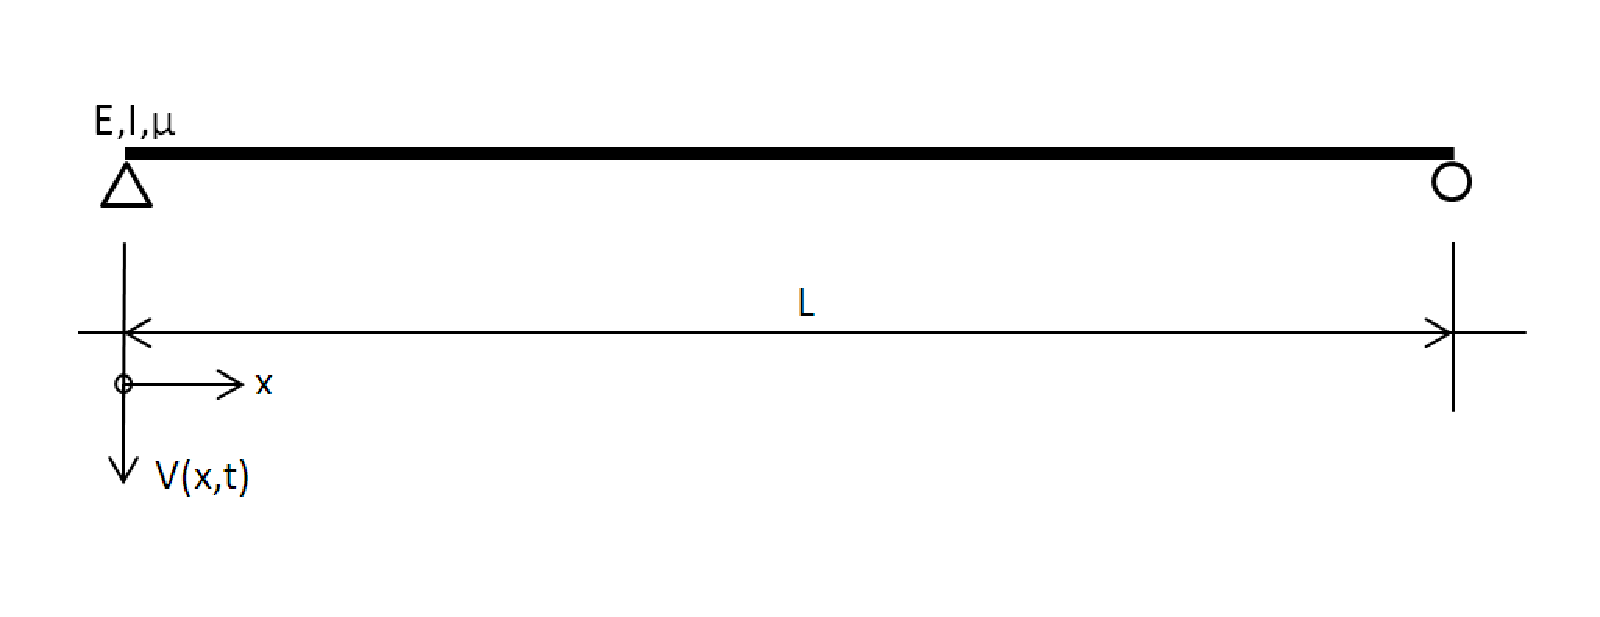
\includegraphics[width=0.8\textwidth]{massbeammodel.pdf}
% 	\caption{Mass beam model of span L}
% 	\label{fig:massbeammodel}
% \end{figure}

% \begin{equation}
% 	EI\dfrac{\partial^4v(x,t)}{\partial x^4}+\mu \dfrac{\partial^2 v(x,t)}{\partial t^2} + 2\mu \omega_b \dfrac{\partial v(x,t)}{\partial t} = f(x,t)
% 	\label{eq:massbeammodel}
% \end{equation}

% where:
% \begin{enumerate}[]
% 	\item $ v(x,t) $:vertical deflection of the beam at the point $ x $ and at time $ t $
% 	\item $ E $:modulus of elasticity of the beam
% 	\item $ I $:moment of inertia of beam cross section
% 	\item $ \mu $:mass per unit length of the beam
% 	\item $ \omega_b $:circular frequency of viscous damping
% 	\item $ f(x,t) $:load at point $ x $ and time $ t $ per unit length of the beam
% \end{enumerate}

% \subsection{Continuous beam}
% The continuous beam model is suitable for multi-span bridges in general. The equation of motion is the same as simple beam model in Equation\ref{eq:massbeammodel}. 

% \begin{figure}[h]
% 	\centering
% 	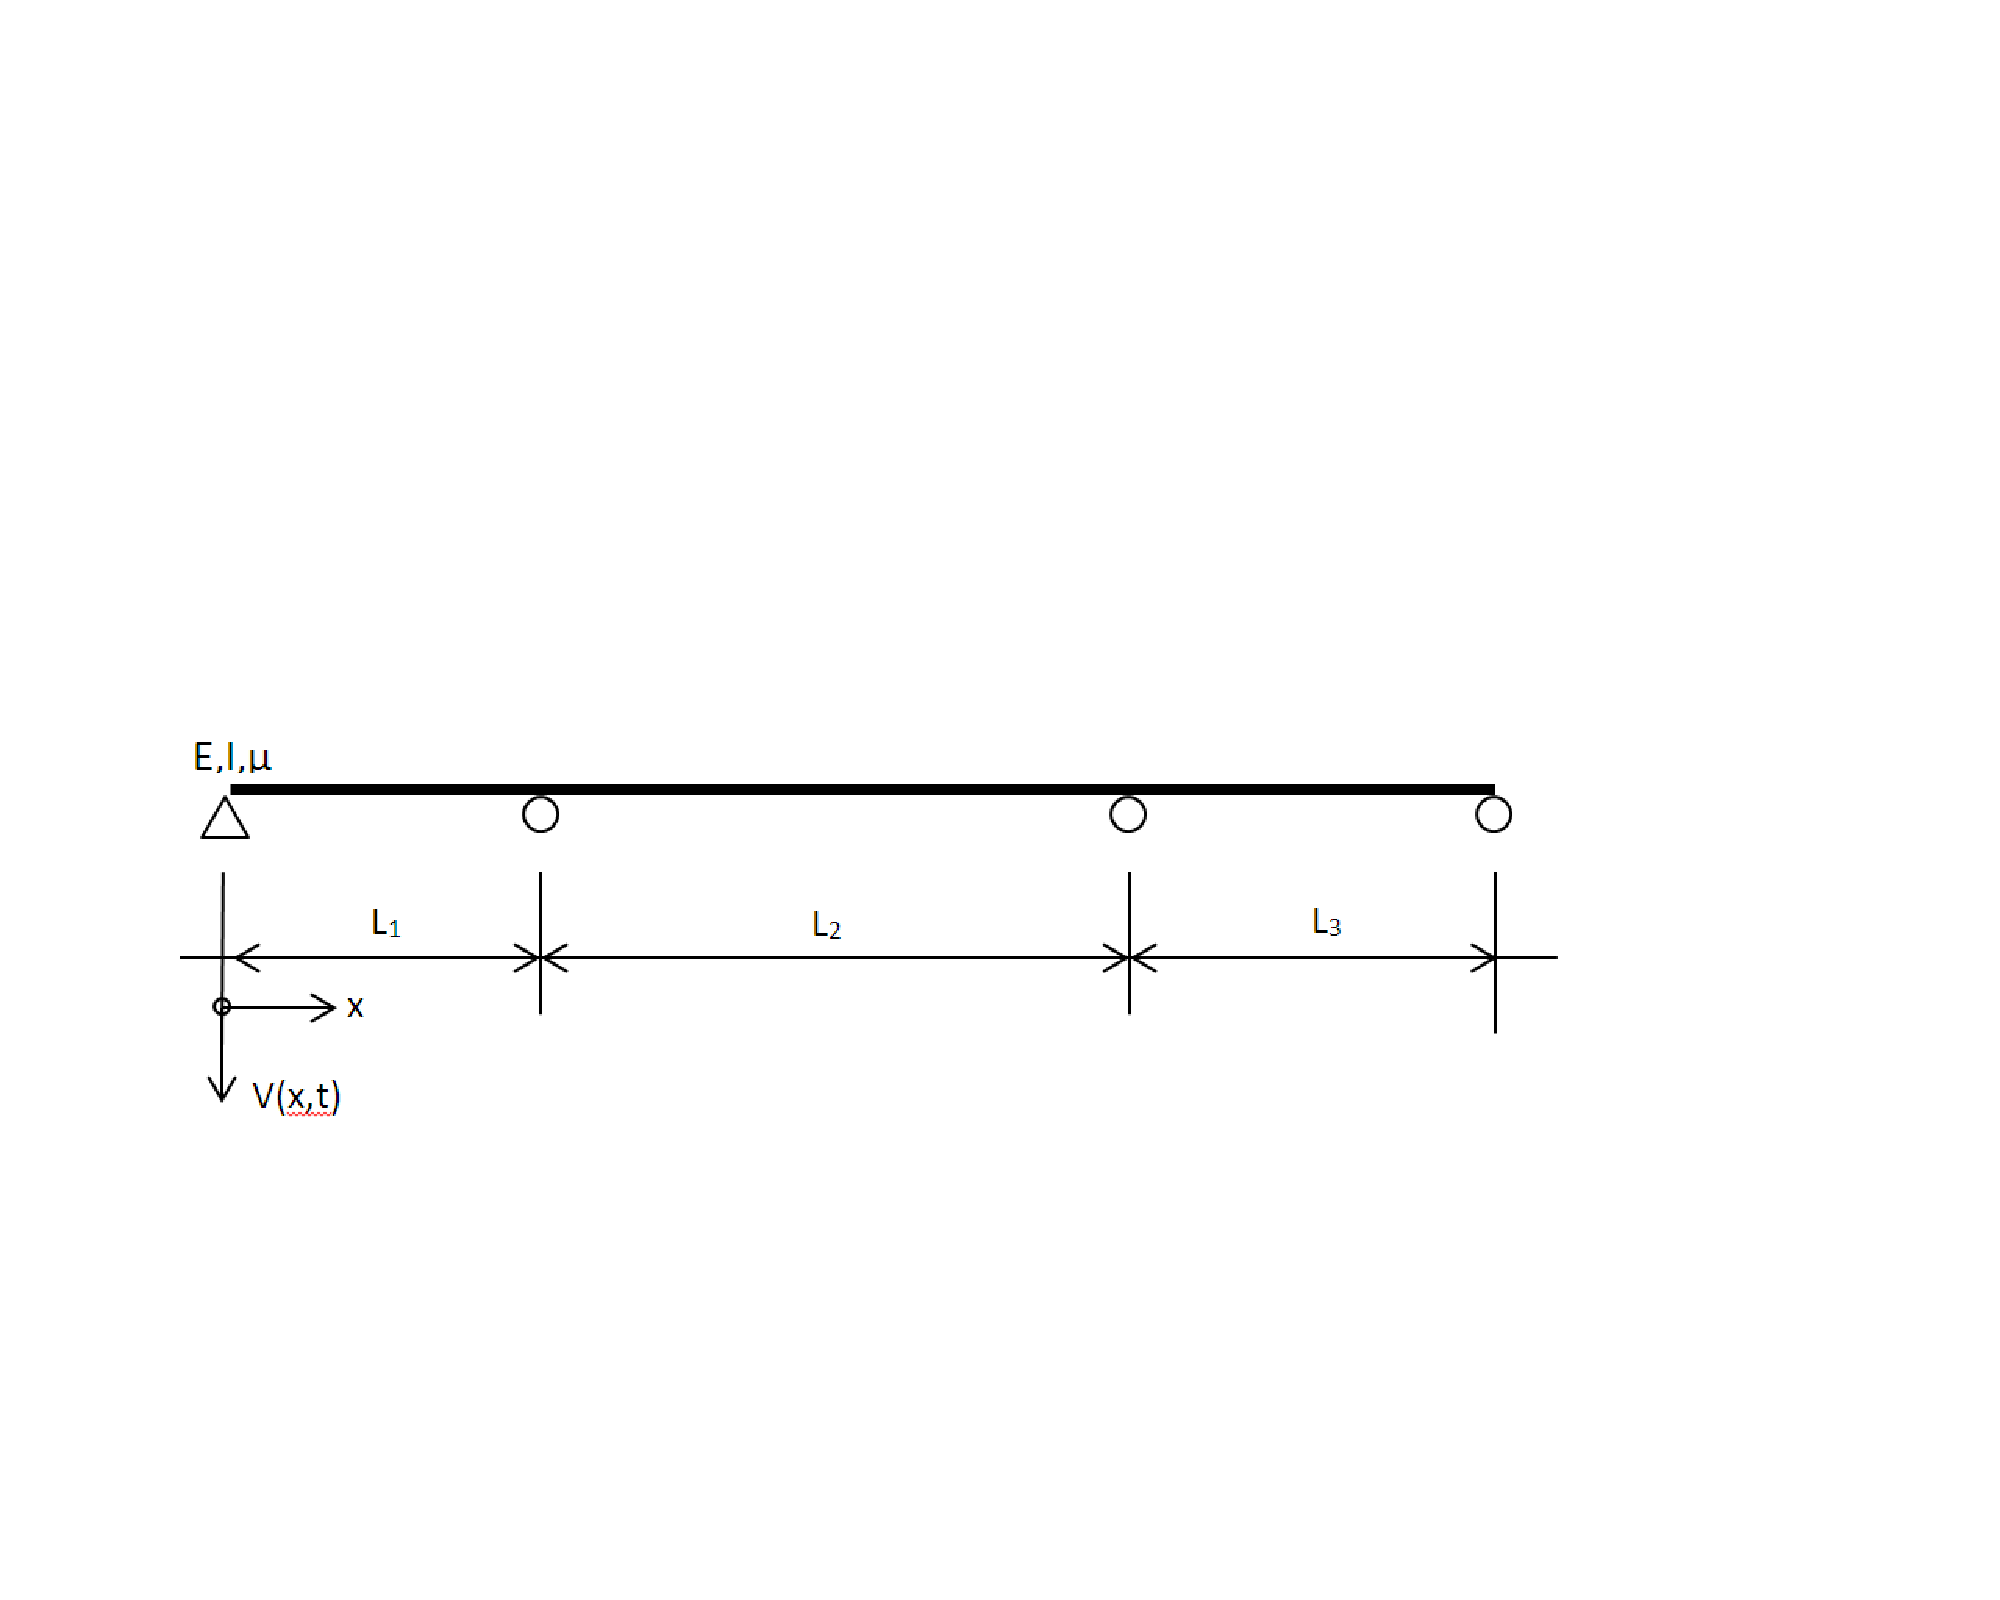
\includegraphics[width=0.8\textwidth]{continuousbeammodel.pdf}
% 	\caption{Continuous beam model}
% 	\label{fig:continuousbeammodel}
% \end{figure}
	
% \subsection{Complex systems}

% \subsubsection{Trusses}

% \subsubsection{Frames}

% \subsubsection{Curved bars}

% \subsection{High strength steel bridges}
% The advantage of high strength steel bridges are

% \begin{enumerate}
% 	\item High quality material
% 	\item Speed of construction
% 	\item Versatility
% 	\item Modification and repair
% 	\item Recycling
% 	\item Durability
% 	\item Aesthetics
% \end{enumerate}

% \cite{macdougall2004state}: Use of high-strength steels for bridge construction in Japan dates back to the 1960s. Several hundred bridges been constructed using 500MPa and 600MPa yield strength steel, and steel with a normal yield strength of 800 MPa has also been used on several projects. In Europe, a variety of high-strength steels with yield strength from 460MPa to 690MPa are available for bridge applications. European structural steel standard EN 10025: 2004 grade S460ML, which has a nominal yield strength of 460MPa, can be welded at room temperature for plate thickness up to 90mm and has a specified minimum Charpy V-notch(CVN) evergy of 27 J at -50$^\circ$C.

% \section{Modelling of railway vehicles}
% According to Newton's law, 2 basic load effects are produced by moving train: vertical forces due to vehicle weight, and inertia effects caused by vehicle acceleration. The loads on a railway bridge are very complex problems thus in engineering practice, loads are often simplified. But, the simplification depends on the purpose of the analysis. 

% \subsection{Moving vertical forces model}
% If the inertia effects are neglected, loads of the moving trains can be modelled as moving vertical forces. For example, load diagram for type TALGO trains is shown in Figure.\ref{fig:verticalmodel} proposed by \cite{uic}.

% \begin{figure}[h]
% 	\centering
% 	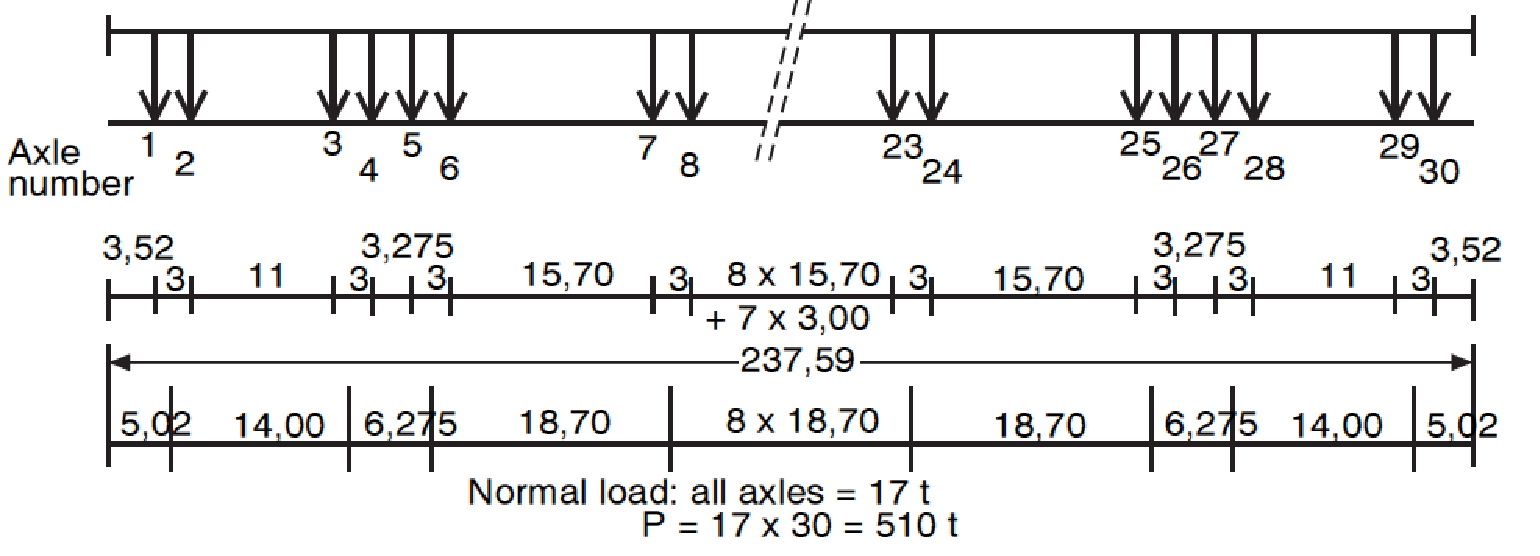
\includegraphics[width=0.8\textwidth]{verticalmodel.pdf}
% 	\caption{Moving vertical force model for TALGO trains}
% 	\label{fig:verticalmodel}
% \end{figure}

% \subsection{Advanced models}
% Nowadays more and more models have been proposed to meet different requirements of railway bridge dynamic analysis. The complexity of these models differs from each other but they are all more complicated than moving vertical forces models. For example, vehicle-bridge interaction model takes vehicle suspension system into account, which gives an alternative for discovering resonance effects between bridge and the vehicle suspension systems. 

% See Figure.\ref{fig:advancedmodel} for an example of advanced model.

% \begin{figure}[p]
% 	\centering
% 	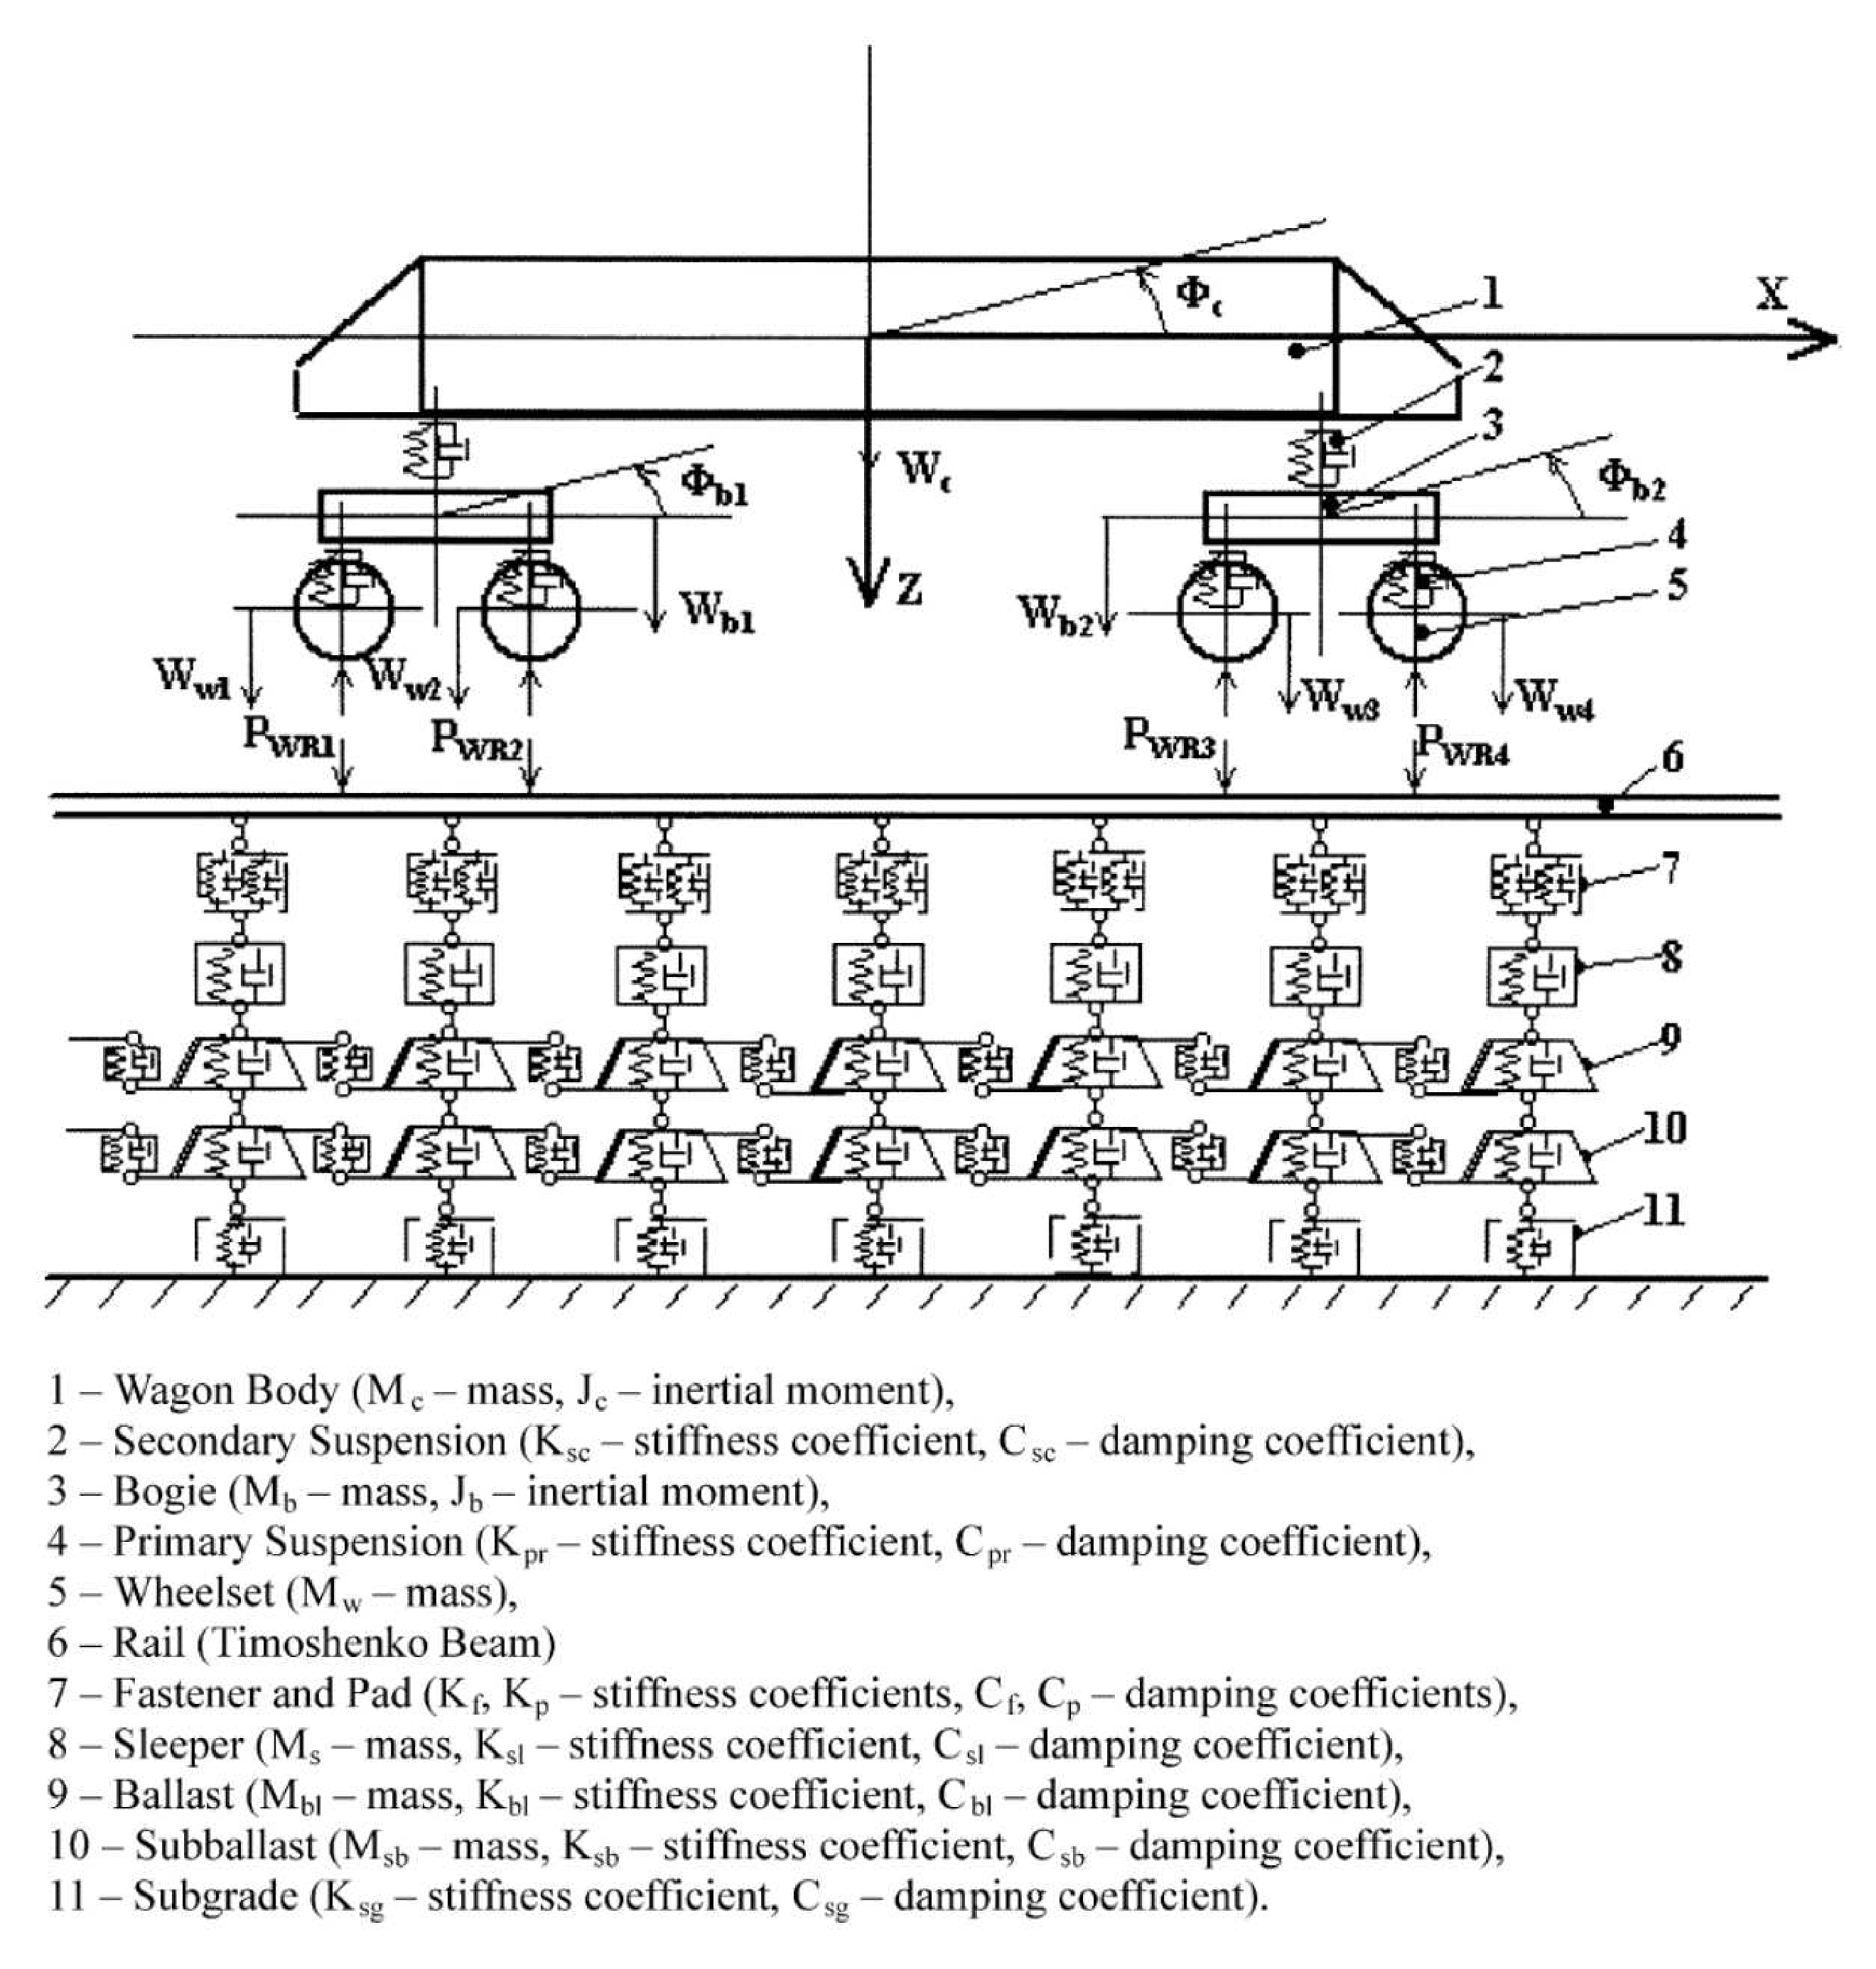
\includegraphics[width=0.8\textwidth]{advancedmodel.pdf}
% 	\caption{A dynamic model for the vertical interaction of the rail track and wagon system. Proposed in \cite{sun2002dynamic}}
% 	\label{fig:advancedmodel}
% \end{figure}


% \subsection{Models proposed in Eurocodes}

% See Chapter~\ref{sec:train-models}

% \section{Track model}
% Proposed in \cite[A.6.1.3]{uic}, the track is represented by Timoshenko beam elements for the rails and takes account of the rail/sleeper fastening characteristics as well as the ballast(if one exists).

% \textit{``A sleeper is generally represented by two beam elements, with two covering the rail and one used for the deck. Sleepers and ballast are modelled as concentrated masses. They are linked to the nodes of the rail and the bridge by a parallel spring and damper system. The track can be modelled to any length on both side of the bridges, where the stiffening effect of the bridge has to be taken into account. The effects of track distribution are not considered. Each vehicle is able to absorb the kinetic energy of the bridge and it is for this reason that, at resonance, the deflections and accelerations of the bridge obtained with this model are lower than those obtained with a live load diagram."}

% The most complete model for analysing train/track/bridge interaction is shown in Figure

% \begin{figure}[h]
% 	\centering
% 	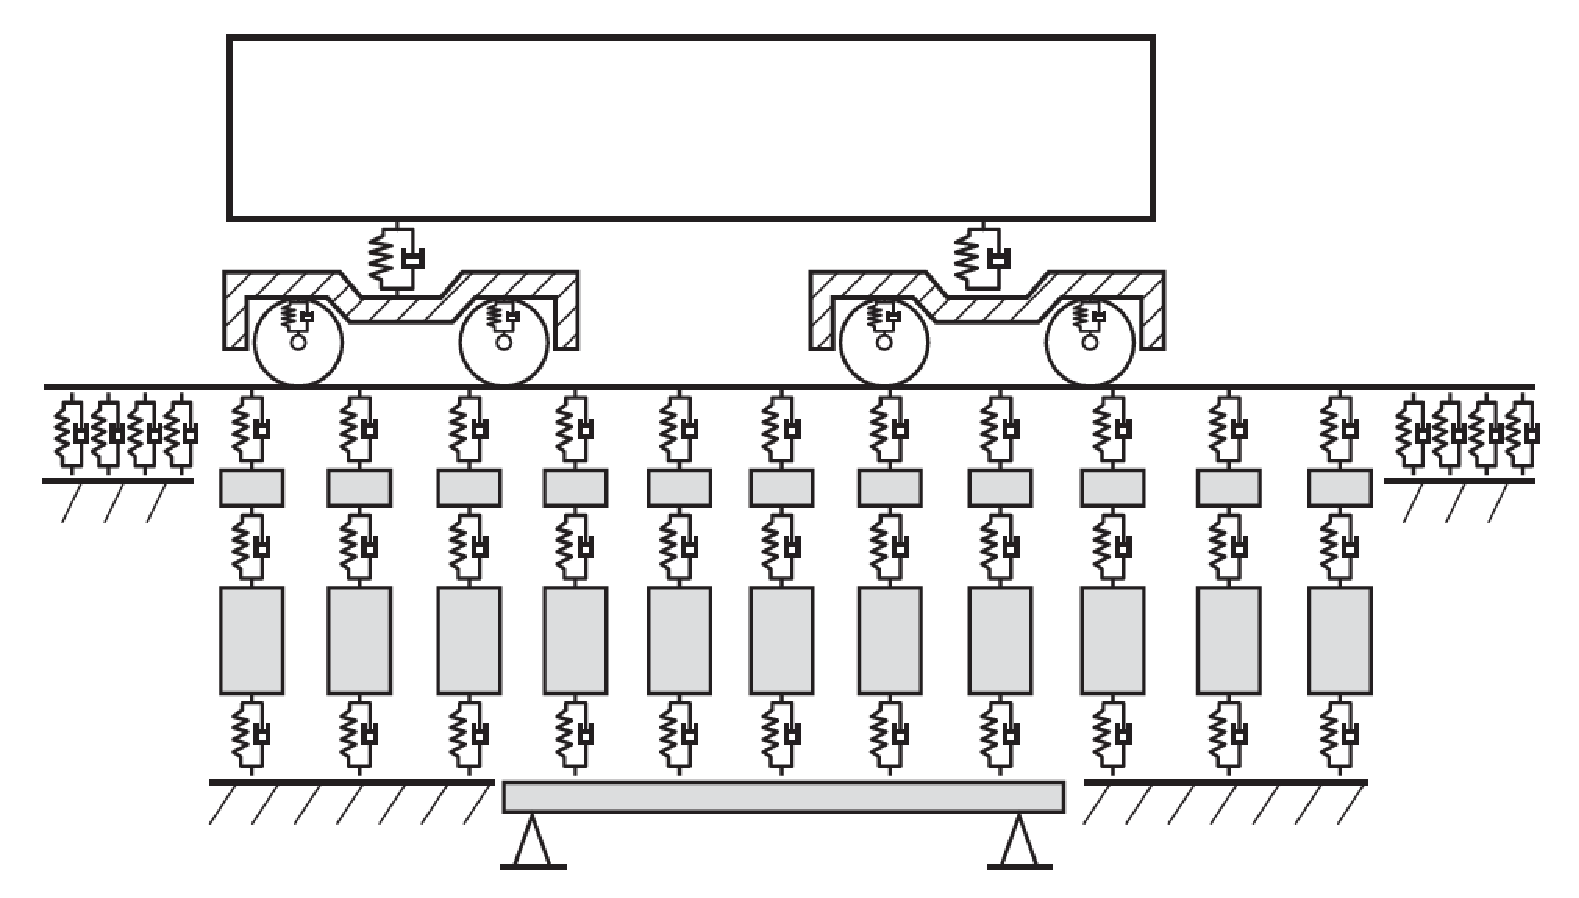
\includegraphics[width=0.8\textwidth]{trackmodel.pdf}
% 	\caption{Diagram of the dynamic train-track-bridge model. Extracted from \cite[Fig. 15]{uic}}
% 	\label{fig:trackmodel}
% \end{figure}


% \section{General design principles and procedures concerning railway bridge dynamics proposed by Eurocodes } \label{designprocedures}


% \subsection{Requirements for railway bridge verification}
% \cite{EC0} propose following requirements


% \begin{enumerate}
% 	\item Checks on bridge deformations shall be performed for traffic safety purposes for the following items:
% 	\begin{enumerate}[-]
% 		\item vertical accelerations of the deck
% 		\item vertical deflection of the deck throughout each span
% 		\item unrestrained uplift at the bearings(to avoid premature bearing failure)
% 		\item vertical deflection of the end of the deck beyond bearings(to avoid destabilising the track, limit uplift forces on rail fastening systems and limit additional rail stresses) 
% 		\item twist of the deck measured along the centre line of each track on the approaches to a bridge and across a bridge(to minimise the risk of train derailment)
% 		\item rotation of the ends of each deck about a transverse axis or the relative total rotation between adjacent deck ends(to limit additional rail stresses, limit uplift forces on rail fastening systems and limit angular discontinuity at expansion devices and switch blades)
% 		\item longitudinal displacement of the end of the upper surface of the deck due to longitudinal displacement and rotation of the deck end(to limit additional rail stresses and minimise disturbance to track ballast and adjacent track formation)
% 		\item horizontal transverse deflection(to ensure acceptable horizontal track radii)
% 		\item horizontal rotation of a deck about a vertical axis at ends of a deck (to ensure acceptable horizontal track geometry and passenger comfort)
% 		\item limits on the first natural frequency of lateral vibration of the span to avoid the occurrence of resonance between the lateral motion of vehicles on their suspension and the bridge
% 	\end{enumerate}
% 	\item Checks on bridge deformations should be performed for passenger comfort, i.e. vertical deflection of the deck to limit coach body acceleration in accordance with A2.4.4.3\cite{EC0}
% 	\item The limits given in A2.4.4.2 and A2.4.4.3\cite{EC0} take into account the mitigating effects of track maintenance (for example to overcome the effects of the settlement of foundations, creep, etc.) 
% \end{enumerate}

% \subsection{Conceptual check}
% The conceptual check is to help designers avoid unsafe designs in conceptual stage. Once the bridge type and rough geometry is sketched, designers can easily know whether the bridge would have dynamic problem in the future. 

% For example, in  \cite[cl.8.7.4]{calgaro2010designers}, it is stated that if the bridge meets criteria ~\ref{cr:nocheck} , no dynamic analysis in necessary. 

% \begin{equation}
% 	\label{cr:nocheck}
% 	V>200km/h \quad \delta_{dyn} \leq \text{ value given by the dynamic study, but }\delta_{stat}\leq L/2600
% \end{equation}

% On the other hand, no other conceptual check criterion is given for train speed under 200km/h. Since there is higher possibility that, for bridges with span larger than 100m, they will have resonance with the normal trains. 

% \subsection{Logic diagram}

% This logic diagram is used to determine whether a dynamic analysis is required, as shown in Figure~\ref{fig:logicdiagram}, is represented in \cite{EC12} Chapter 6.4 Dynamic Effects, where $V [Km/h]$ is the Maximum Line Speed at the site, $L [m]$, the span length, $n_0 [Hz]$, the first nature frequency under permanent loads, $n_T$, the first natural torsional frequency for the same load, $v [m/s]$ the maximum nominal speed and finally $(v/n_0)_{lim}$, as given in Annex F of EN1991-2. The frequency first of vibration, $n_0$, must be within the limits established in figure~\ref{fig:frequencylimit}.

% Checking through the logic diagram is regarded as first step is because designers can try to avoid designs that will be required to be dynamic analysed in the very beginning of the designing phase. 

% The upper limit (1) is defined as

% \begin{equation}
% 	n_0=94,76L^{-0,748}
% \end{equation}

% % and the lower limit (2) as:

% \begin{equation}
% 	n_0= \{ \begin{array}{ll}
% 	80/L & \mbox{for $4m\leq L \leq 20m$} \\
% 	94,76L^{-0,748} & \mbox{for $20m\leq L \leq 100m$}
% \end{array} 
% \end{equation}

% \begin{figure}[h]
% \centering
% 	\begin{subfigure}[b]{0.45\textwidth}
%     	\centering
%     	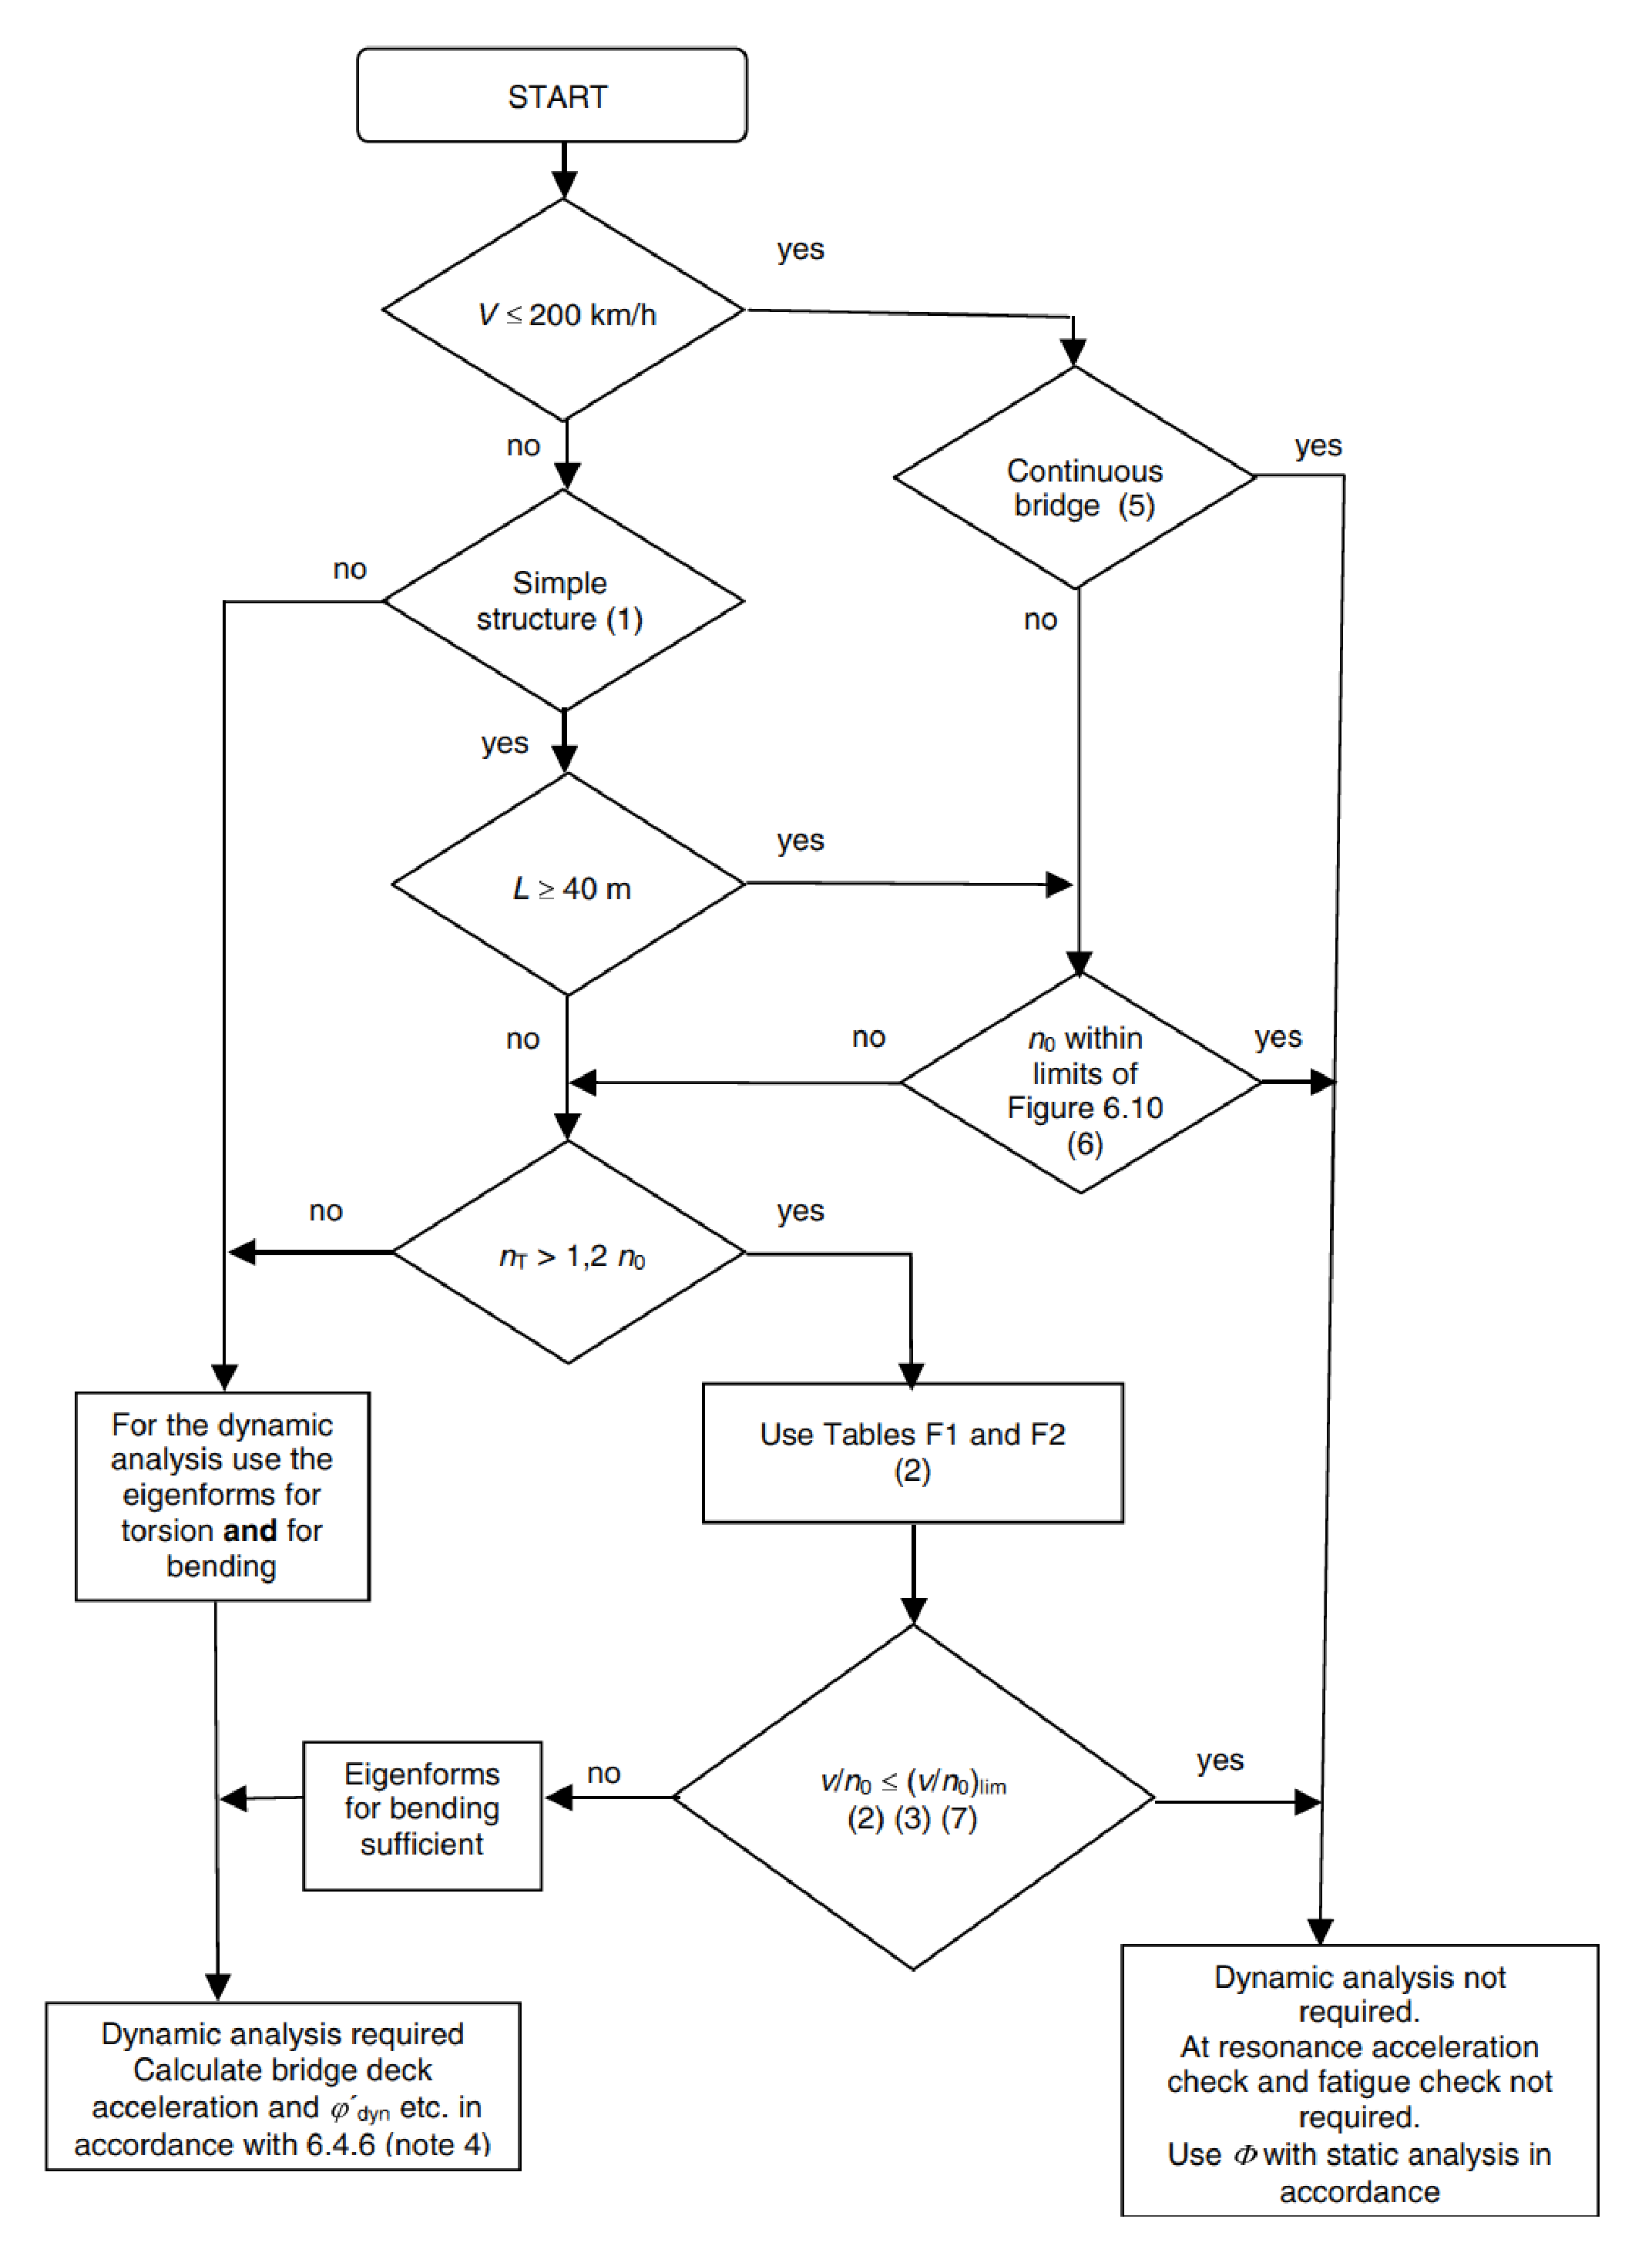
\includegraphics[width=\textwidth]{logicdiagram.pdf}
%     	\caption{Flow chart for determining whether a dynamic analysis is required. Extracted from EN1991-2\cite{EC12}}
%     	\label{fig:logicdiagram}
% 	\end{subfigure}
% 	\begin{subfigure}[b]{0.45\textwidth}
%     	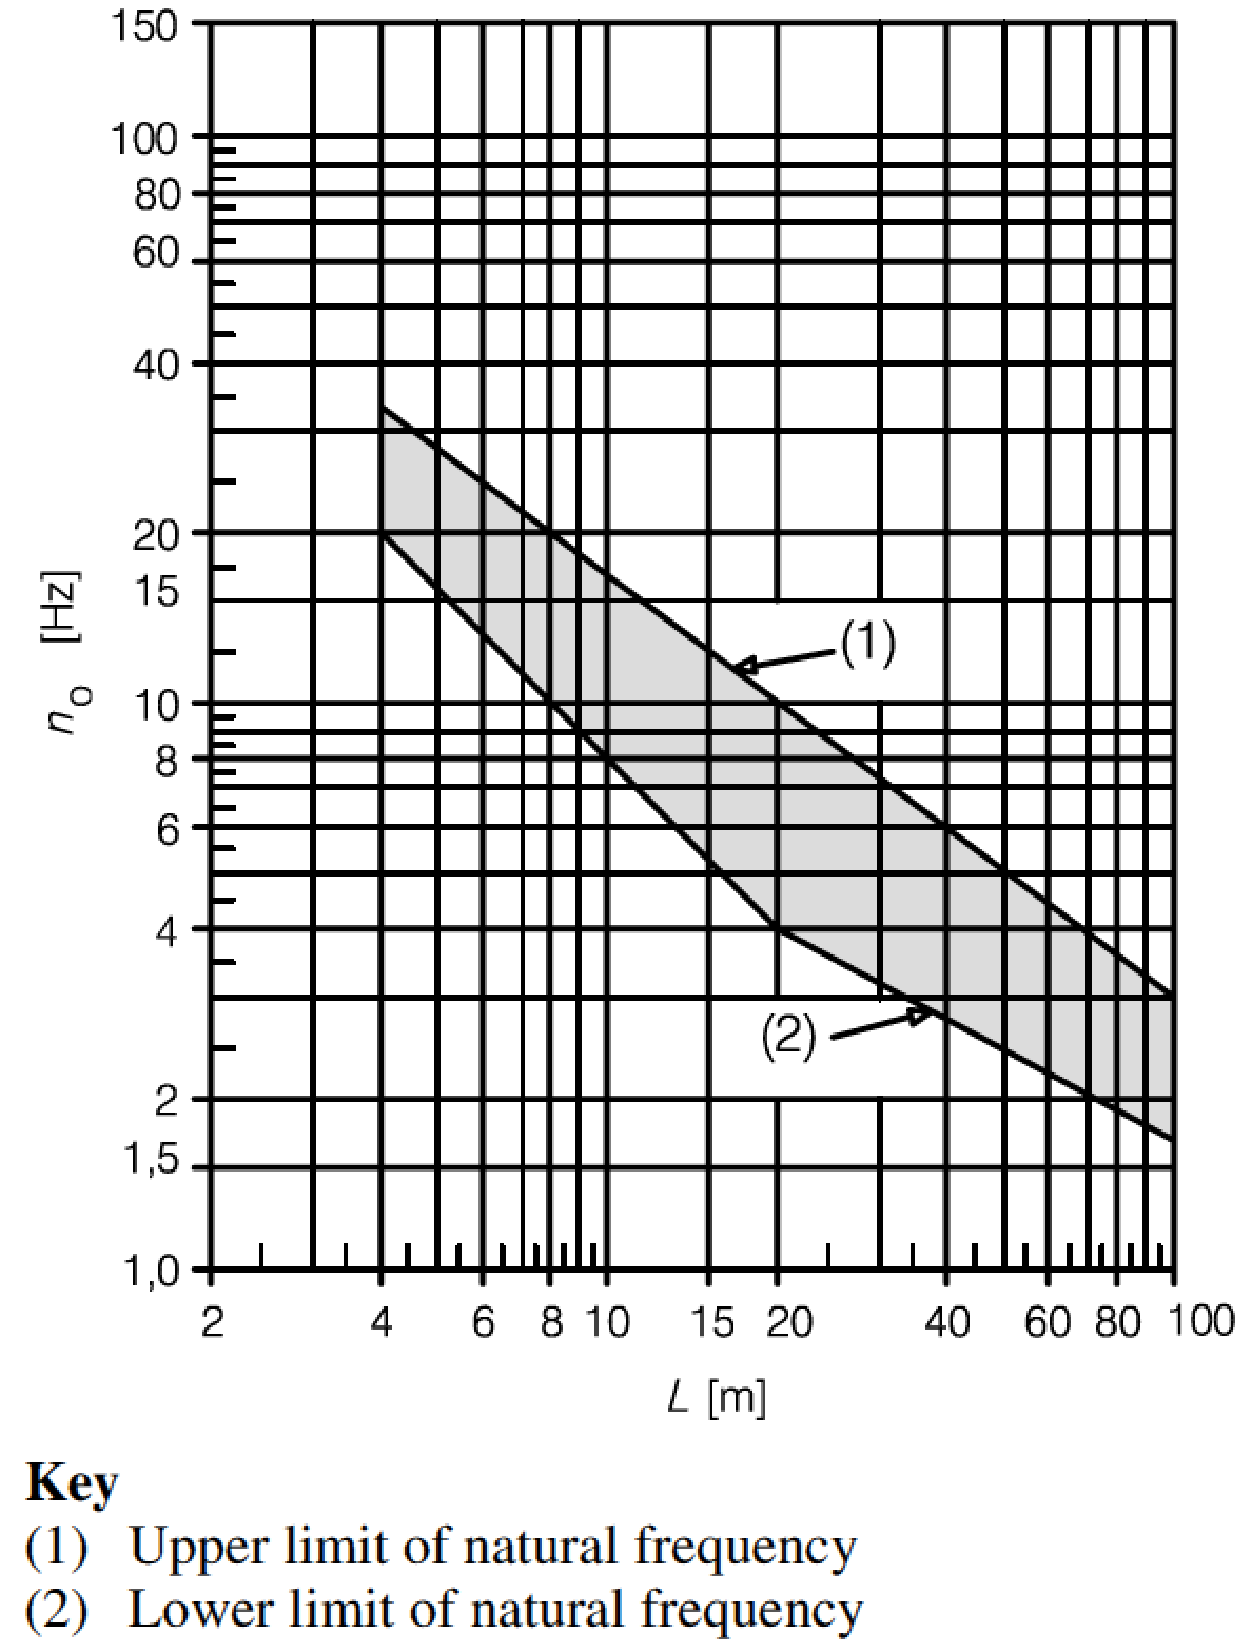
\includegraphics[width=\textwidth]{frequencylimit.pdf}
%     	\caption{Limits for bridge natural frequencies, $n_0 [Hz]$, as a function $L [m]$. Extracted from EN1991-2\cite{EC12}.}
%     	\label{fig:frequencylimit}
% 	\end{subfigure}
% \caption{Logic diagram for determining whether dynamic analyses are necessary, extracted from \cite[6.4.4]{EC12}}
% \label{logicandlimit}
% \end{figure}

% \subsection{Train models}\label{sec:train-models}
% According to NEN 1991-2\cite{EC12} and Designers Guide\cite{calgaro2010designers} Rail traffic actions are defined by means of load models, Four models of railway loading are given:
% \begin{enumerate}[$\bullet$]
% 	\item LM71 and LM SW/0(for continuous bridges) to represent normal rail traffic on mainline railways (passenger and heavy freight traffic)
% 	\item SW/2 to represent abnormal loads or waggons
% 	\item LM 'unloaded train' to represent the effect of an unloaded train
% 	\item LM HSLM (comprising HSLM-A and HSLM-B) to represent the loading from passenger trains at speeds exceeding 200km/h.
% \end{enumerate}

% \subsubsection{Load Model 71}
% LM71 represents the static effect of vertical loading due to normal rail traffic.

% The load arrangement and the characteristic values for vertical loads have to be taken as shown in Figure.~\ref{lm71}

% The actions listed below, associated with LM71, have to be multiplied by factor $ \alpha $:

% \begin{enumerate}[-]
% 	\item equivalent vertical loading for earthworks and earth pressure effects
% 	\item centrifugal forces
% 	\item nosing force (multiplied by $ \alpha $ for $ \alpha\geq 1 $ only)
% 	\item traction and braking forces
% 	\item derailment actions for accidental design situations
% 	\item Load Model SW/0 for continuous span bridges
% \end{enumerate}

% \textit{For international lines, it is recommended that a value of $ \alpha \geq 1.0 $ is adopted. But this freedom of choice of the factor $ \alpha $ could lead to a non-uniform railway network in Europe. Therefore in UIC Code 702\textsuperscript{4} $ \alpha=1.33 $ is generally recommended for all new bridges constructed for the international freight network, but not compulsory}. 

% \begin{figure}[h]
% 	\centering
% 	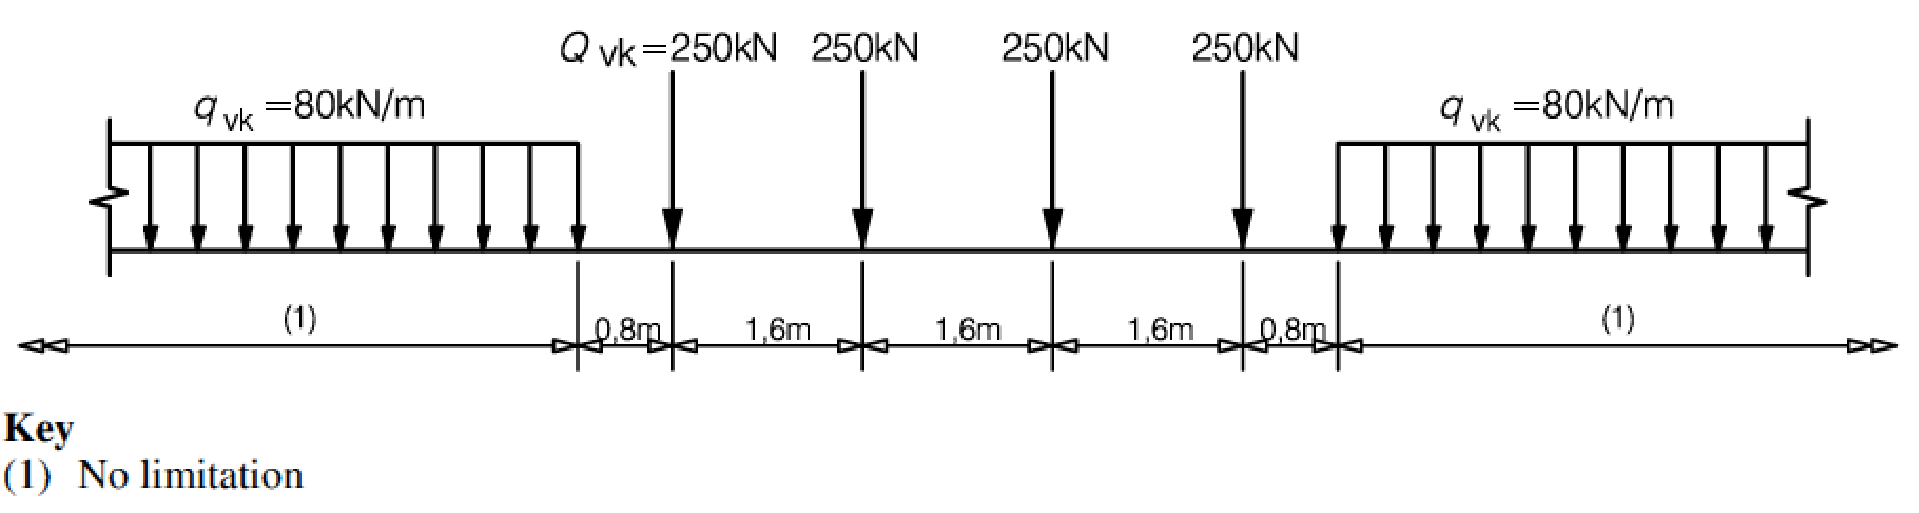
\includegraphics[width=0.8\textwidth]{lm71.pdf}
% 	\caption{Load Model 71 and characteristic values for vertical loads. Extracted from EN1991-2\cite{EC12}}
% 	\label{lm71}
% \end{figure}

% \subsubsection{Load Models SW/0 and SW/2}
% Load Models SW/0 represents the static effect of vertical loading due to normal rail traffic on continuous beams.

% Load Model SW/2 represents the static effect of vertical loading due to heavy abnormal rail traffic. 

% The load arrangement is as shown in Figure.~\ref{lmsw}, with the characteristic values of the vertical loads according to Table.\ref{tab:sw}

% \begin{figure}[h]
% 	\centering
% 	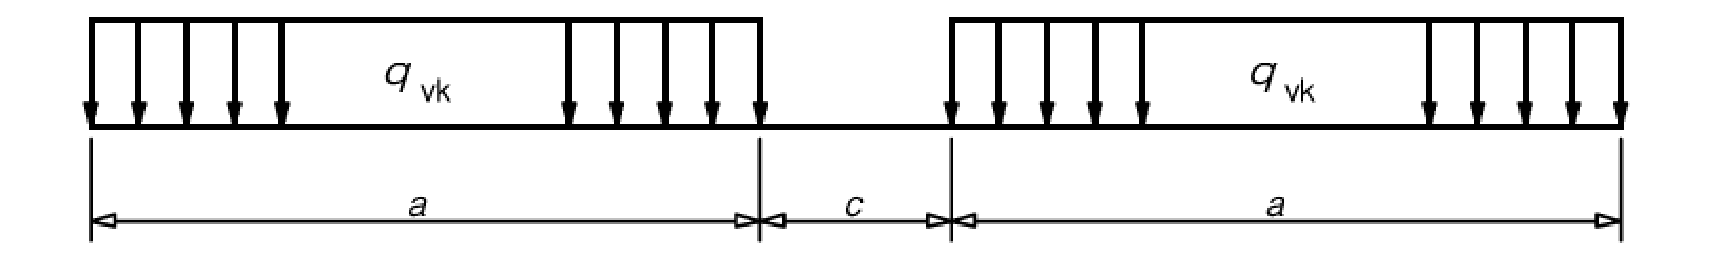
\includegraphics[width=0.8\textwidth]{lmsw.pdf}
% 	\caption{Load Models SW/0 and SW/2.. Extracted from EN1991-2\cite{EC12}}
% 	\label{lmsw}
% \end{figure}

% \begin{table}[h]
% 	\centering
% 	\begin{tabular}{llll}
% 		\hline
% 		Load model & $ q_{vk} (kN/m) $ & $ a (m) $ & $ c (m) $ \\
% 		\hline
% 		SW/0 & 133 & 15.0 & 5.3\\
% 		SW/2 & 150 & 25.0 & 7.0\\
% 		\hline
% 	\end{tabular}
% 	\caption{Characteristic values for vertical loads for Load Models SW/0 and SW/2}
% 	\label{tab:sw}
% \end{table}

% \subsubsection{Load Model 'unloaded train'}
% From some specific verification purposes a specific load model is used, called 'unloaded train'. The Load Model 'unloaded train' consists of a vertical uniformly distributed load with a characteristic value of 10.0kN/m.

% \subsubsection{Load Models SHLM}
% Load Models HSLM comprises two separate universal \textit{high-speed} trains with variable coach lengths. In order to ensure that they deliver dynamic behaviour with regards to current and future train traffic, bridges should be calculated using the Universal Dynamic Train(HSLM) consisting of HSLM-A and/or HSLM-B. These are defined as follows:

% \begin{enumerate}[$ \bullet $]
% 	\item For the definition of train HSLM-A, a set of ten reference trains A1 to A10: see Figure.~\ref{fig:hslma} and Table.~\ref{tab:hslma} below.
% 	\item For the definition of train HSLM-B: See Figure.~\ref{fig:hslmbdiagram} and `\ref{fig:hslmbtable} below
% \end{enumerate}

% \begin{figure}[h]
% 	\centering
% 	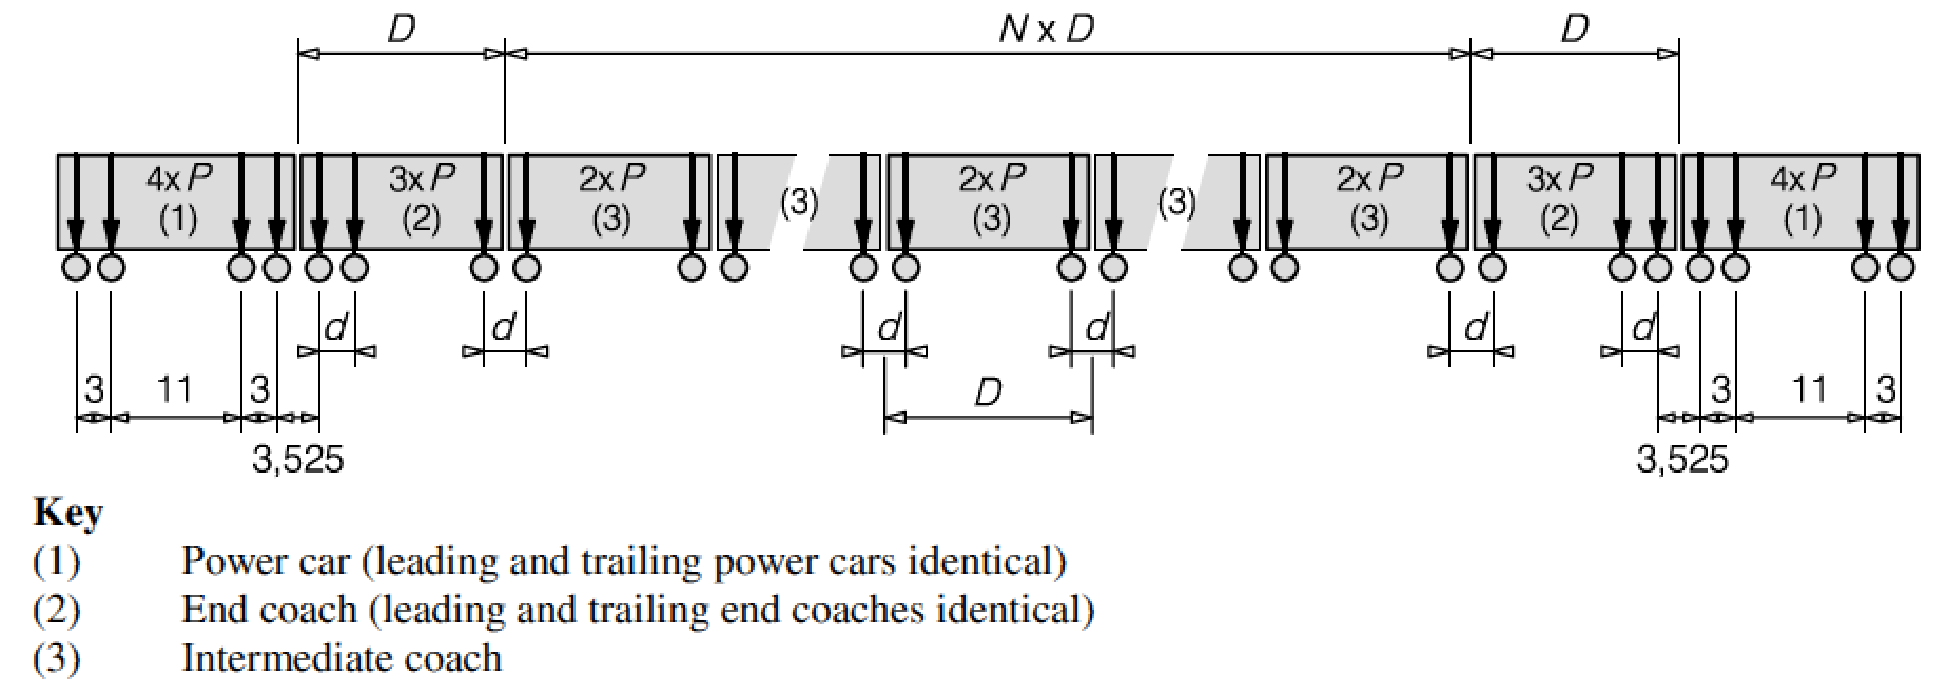
\includegraphics[width=0.8\textwidth]{hslma.pdf}
% 	\caption{Diagram of Universal Dynamic Train HSLM-A. Extracted from EN 1991-2\cite{EC12}}
% 	\label{fig:hslma}
% \end{figure}

% \begin{table}[h]\footnotesize
% 	\centering
% 	\begin{tabular}{p{2cm}p{2cm}p{2cm}p{2cm}p{2cm}}
% 		\hline
% 		Universal train & Number of intermediate coaches, $ N $ & Coach length $ D(m) $ & Bogie axle spacing $ d (m) $ & Point force $ P (kN) $ \\
% 		\hline
% 		A1 & 18 & 18 & 2.0 & 170 \\
% 		A2 & 17 & 19 & 3.5 & 200 \\
% 		A3 & 16 & 20 & 2.0 & 180 \\
% 		A4 & 15 & 21 & 3.0 & 190 \\
% 		A5 & 14 & 22 & 2.0 & 170 \\
% 		A6 & 13 & 23 & 2.0 & 180 \\
% 		A7 & 13 & 24 & 2.0 & 190 \\
% 		A8 & 12 & 25 & 2.5 & 190 \\
% 		A9 & 11 & 26 & 2.0 & 210 \\
% 		A10 & 11 & 27 & 2.0 & 210 \\			
% 		\hline		
% 	\end{tabular}
% 	\caption{HSLM-A, definition of ten trains. Extracted from EN1991-2\cite{EC12}}
% 	\label{tab:hslma}
% \end{table}

% \begin{figure}[h]
% 	\centering
% 	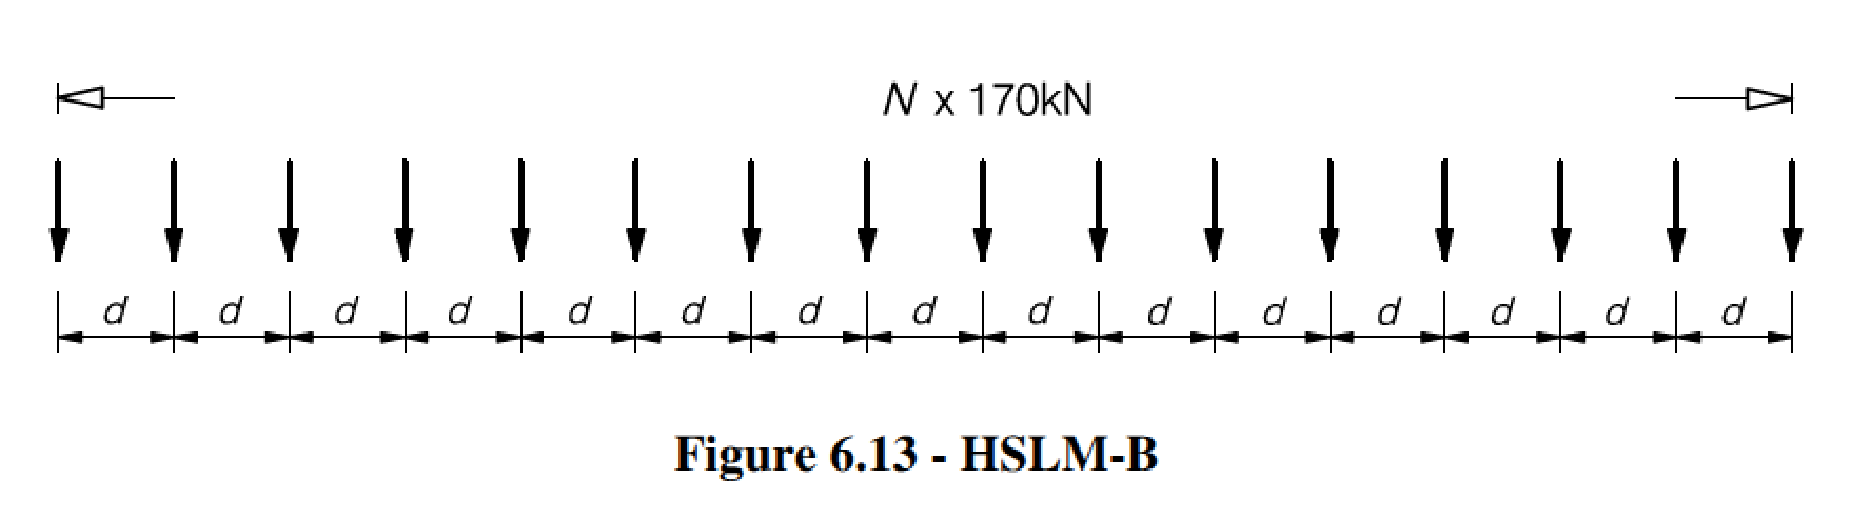
\includegraphics[width=0.8\textwidth]{hslmb.pdf}
% 	\caption{Diagram of Universal Dynamic Train HSLM-B. Extracted from EN 1991-2\cite{EC12}}
% 	\label{fig:hslmbdiagram}
% \end{figure}

% \begin{figure}[h]
% 	\centering
% 	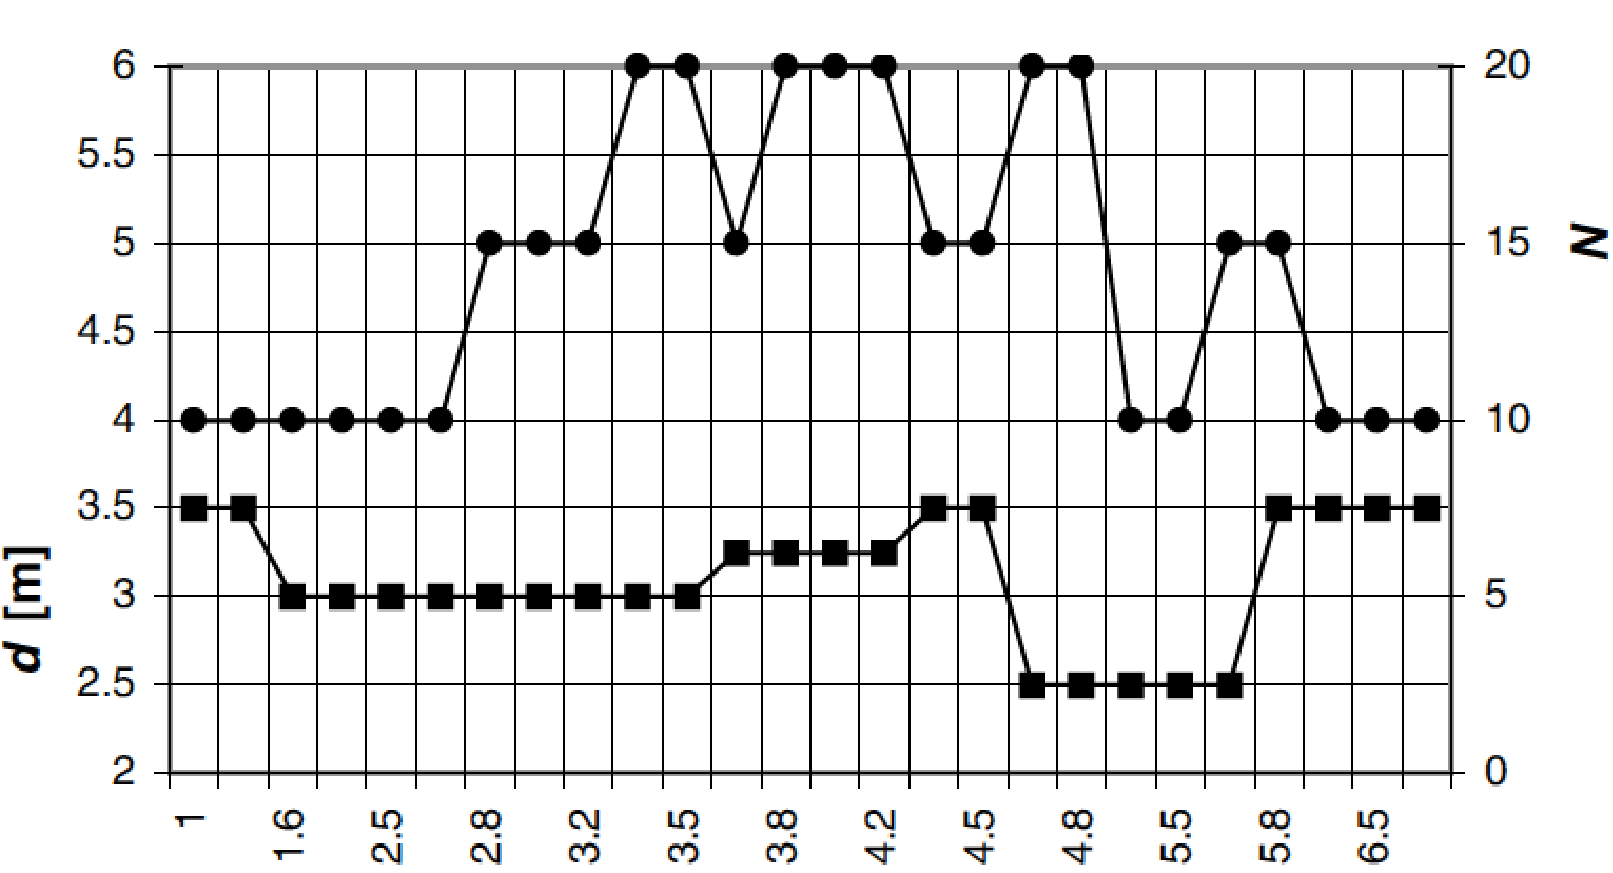
\includegraphics[width=0.8\textwidth]{hslmb2.pdf}
% 	\caption{Universal Dynamic Train HSLM-B. Extracted from EN 1991-2\cite{EC12}}
% 	\label{fig:hslmbtable}
% \end{figure}

% This Load Model comprises $ N $ number of point forces of 170kN at regular spacing $ d(m) $ (\ref{fig:hslmbdiagram}) where $ N $ and $ d $ are defined in Figure.~\ref{fig:hslmbtable}

% Table.~\ref{hslmapplication} illustrates how HSLM-A and HSLM-B are applied and indicates the train to be used for dynamic bridge calculations.

% \begin{table}[h] \scriptsize
% 	\begin{tabular}{lll}
% 		\hline
% 		Structural configuration & \multicolumn{2}{c}{Span} \\
% 		& $ L<7m $ & $ L\geq 7m $ \\
% 		\hline
% 		Simply supported span & HSLM-B & HSLM-A \\
% 		Continuous structure or Complex Structure & Trains A1 to A10 inclusive & Trains A1 to A10 inclusive\\
% 	\end{tabular}
% 	\caption{Application of HSLM-A and HSLM-B. Data extracted from EN 1991-2\cite{EC12}}
% 	\label{hslmapplication}
% \end{table}

% \subsection{Dynamic factor}\label{sec:dynamicfactor}
% The dynamic factor $ \Phi $ takes account of the dynamic magnification of stress and vibration effects in the structure but does not take account of resonance effects.

% Generally the dynamic factor $ \varPhi $ is taken as either $ \varPhi_2 $ or $ \varPhi_3 $ according to the quality of track maintenance as follows:

% \begin{enumerate}[(a)]
% 	\item For Carefully maintained track: 
% 		\begin{equation}
% 			\varPhi_2=\dfrac{1.44}{\sqrt{L_\varPhi}-0.2}+0.82 \quad with1.00\leq \varPhi_2\leq 1.67
% 		\end{equation}
% 	\item For track with standard maintenance:
% 		\begin{equation}
% 			\varPhi_3=\dfrac{2.16}{\sqrt{L_\varPhi}-0.2}+0.73 \quad with 1.00\leq \varPhi_3\leq 2.0
% 		\end{equation}\\
% 	where $ L_\varPhi $ is the `determinant' length (length associated with $ \varPhi $ ) in metres as defined in Table 6.2, EN1991-2\cite{EC12}.
% \end{enumerate}

\subsection{Nosing force}\label{sec:nosingforce}
Nosing force is defined in Eurocode 1991-2. Its original background can be found in \cite[Proposed criteria]{d181}. It is defined as a representation of actions, in combine with actions like vertical loads, dynamic effects, centrifugal forces, traction and braking forces, etc.

The evidence of RP6 is the background of nosing force in EN1991-2 is the following repeating literature:

In \cite[6.5.2]{EC12}:
\begin{quote}
	(1)P The nosing force shall be taken as a concentrated force acting horizontally, at the top of the rails, perpendicular to the centre-line of track. It shall be applied on both straight track....
\end{quote}

In \cite[4.1B]{d181}:
\begin{quote}
	These forces shall be applied at the top of the rails in the most unfavourable position and acting horizontally, perpendicular to the track centreline...
\end{quote}

With another statement also helps proofing RP6 is the background of nosing force in EN1991-2 in \cite[4:Draft Recommendations]{d181}:

\begin{quote}
	These can therefore be expressed as follows: (Article \textbf{6.5.2} of ENV 1991-3 of 1994)...
\end{quote}

ENV 1991-3 was renamed to EN 1991-2 in 2003.

Originally in \cite[4:Draft Recommendations]{d181}, nosing forces was defined as lateral forces from vehicle/bridge interaction as a result of \textbf{hunting}.

The characteristic value of the nosing force shall be taken as $Q_{sk} = 100kN$. It shall not be multiplied by the factor $\Phi$ (\cite[6.45]{EC12}) or by the factor $f$ in \cite[6.51]{EC12}. 

The characteristic value of the nosing force should be multiplied by the factor $\alpha$ in accordance with \cite[6.3.2]{EC12} for values of $\alpha \geq 1$

The nosing force shall always be combined with a vertical traffic load.

A detailed analysis on the background of nosing force will be given in Section.\ref{sec:lateralforce329}

% \subsection{Static analysis}
% A static analysis shall be carried out with the load models defined in Section Load Models(LM71 and where required Load Models SW/0 and SW/2). The result shall be multiplied by the dynamic factor $ \Phi $ (and if required multiplied by $ \alpha $)

% \subsection{Bridge parameters}
% In designers' guide\cite{calgaro2010designers}, bridge parameters on dynamic effects are discussed.

% \subsubsection{Structural damping}
% Structural damping is a key parameter in dynamic analysis. The magnitude of the vibrations depends heavily on structural damping, especially in proximity to resonance.

% \subsubsection{Mass of the bridge}
% Maximum dynamic effects occur at resonance peaks, where a multiple of the load frequency coincides with the natural frequency of the structure. Underrating the mass will lead to over-estimation of the natural frequency of the structure and of the speed at which resonance occurs.

% \subsubsection{Stiffness of the bridge}
% Maximum dynamic load effects are likely to occur at resonant peaks when a multiple of the frequency of loading and a natural frequency of the structure coincide. Any overestimation of bridge stiffness will overestimate the natural frequency of the structure and speed at which resonance occurs; it provides conservative results.

% \section{Dynamic analysis}
% EN 1991-2\cite{EC12} doesn't specify the method of dynamic analysing, but UIC Leaflet 776\textsuperscript{2}\cite{uic} indicates that  for normal bridges there are 4 methods of analysing(an approximate method and three simplified method). However, 776\textsuperscript{2}\cite{uic} also indicates for special structures (bridges with long spans such as bowstring bridges), have to be solved using generic finite element (FEM) programs.

% Analysing using FEM programs can be very time and money consuming providing a complicated structure. Fortunately UIC Leaflet 776\textsuperscript{2}\cite{uic} is an optional reference so FEM analysing is not required in EN 1991-2 \cite{EC12}. Thus finding a simplified way of analysing complicated bridge structures is vital. The development of dynamic analysing methods will be discussed in Chapter.\ref{sec:dynamic-analysing-methods}

\subsection{Verification of the Limit States}
\cite[6.4.6.5]{EC12} proposes following principles to be followed during design:

To ensure traffic safety:
\begin{enumerate}
	\item The verification of maximum peak deck acceleration shall be regarded as a traffic safety requirement checked at the serviceability limit state for the prevention of track instability
	\item The dynamic enhancement of load effects shall be allowed for by multiplying the static loading by the dynamic factor $\varPhi$ defined in \cite[6.4.5]{EC12}. If a dynamic analysis is necessary, the results of the dynamic analysis shall be compared with the results of the static analysis enhanced by $\varPhi$ (and if required multiplied by $\alpha$ in accordance with \cite[6.3.2]{EC12}) and the most unfavourable load effects shall be used for the bridge design.
	\item If a dynamic analysis is necessary, a check shall be carried out according to \cite[6.4.6.6]{EC12} to establish whether the additional fatigue loading at high speeds and at resonance is covered by consideration of the stresses due to load effects from $\varPhi \times LM71$ (and if required $\varPhi \times Load Model SW/0$ for continuous structures and classified vertical load in accordance with \cite[6.3.2(3)]{EC12} where required). The most adverse fatigue loading shall be used in the design.  
\end{enumerate}

% \subsection{Ultimate limit states}

\subsection{Serviceability limit states - traffic safety}

% \subsubsection{Vertical accelerations of the deck}
% The maximum peak values for bridge deck accelerations, calculated along each track, shall not exceed the following design values:

% \begin{enumerate}
% 	\item $ 3.5m/s^2 $ for ballasted track
% 	\item $ 5m/s^2 $ for direct fastened track with tracks and structural elements designed for high speed traffic
% \end{enumerate}

% Also, the range of frequencies to take into account in the determination of the dynamic response in terms of accelerations, shall not exceed the maximum of the following values:

% \begin{enumerate}
% 	\item $30Hz$
% 	\item $1.5\times n_0$
% 	\item the frequency of the third mode of vibration of the member in study
% \end{enumerate}

% \subsubsection{Deck twist}
% The twist of the bridge shall be calculated taking into account the characteristic values of Load Model 71 as well as SW/0 or SW/2 as appropriated multiplied by $\phi$ and $\alpha$ and Load Model HSLM including centrifugal effects, all in accordance with EN1991-2, 6. 

% Twist shall be checked on the approach to the bridge, across the bridge and for the departure from the bridge (see A2.4.4.1(2)P).

% The maximum twist $t$ [mm/3m] of a track gauge $s$ [m] of 1.435m measured over a length of 3m(Figure\ref{fig:difinitiondecktwist}) should not exceed the values given in Table:\ref{tab:limitingvaluedecktwist}

% \begin{table}[h]
% 	\centering
% 	\begin{tabular}{cc}
% 		\hline
% 		Speed range $V$ (km/h) & Maximum twist $t$ (mm/3m) \\
% 		\hline
% 		$v\leq 120$ & $t\leq t_1$ \\
% 		$120\leq v \leq 200$ & $t\leq t_2$ \\
% 		$v>200$ & $t\leq t_3$ \\
% 		\hline
% 	\end{tabular}
% 	\\
% 	\raggedright{Note The values for $t$ may be defined in the National Annex.\\ The recommended values for the set of $t$ are:\\ $t_1=4.5$\\$t_2=3.0$\\$t_3=1.5$\\Values for a track with a different gauge may be defined in the National Annex}
% 	\caption{Limiting Values of deck twist}
% 	\label{tab:limitingvaluedecktwist}
% \end{table}
	
% \begin{figure}[h]
% 	\centering
% 	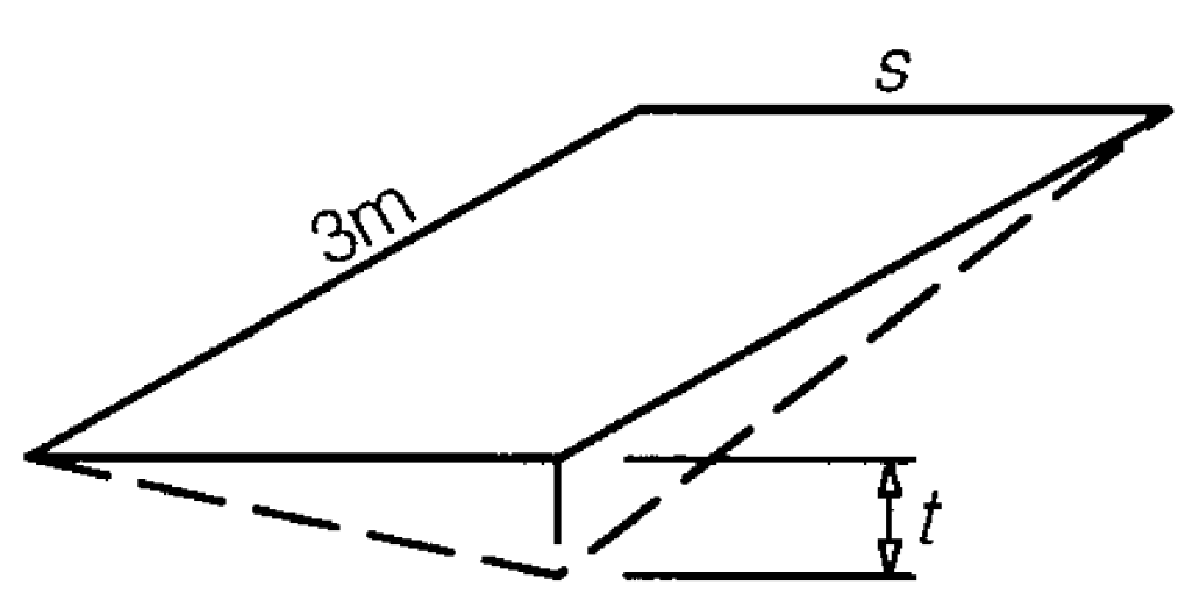
\includegraphics[width=0.8\textwidth]{definitiondecktwist.pdf}
% 	\caption{Definition of deck twist. Extracted from \cite[Figure A2.1]{1990a2}}
% 	\label{fig:difinitiondecktwist}
% \end{figure}

% \paragraph{Vertical deformations}
% For all the structures configurations, loaded with the classified characteristic vertical LM 71, or with the models SW/0 and SW/2 if required, the maximum  total vertical deflection measured along any track due to railway traffic actions should not exceed $L/600$. The angular rotations at the end of decks, represented in Figure.\ref{fig:difinitionangularrotations} , in the vicinity of expansion devices, switches and crossings, should be verified.

% \begin{figure}[h]
% 	\centering
% 	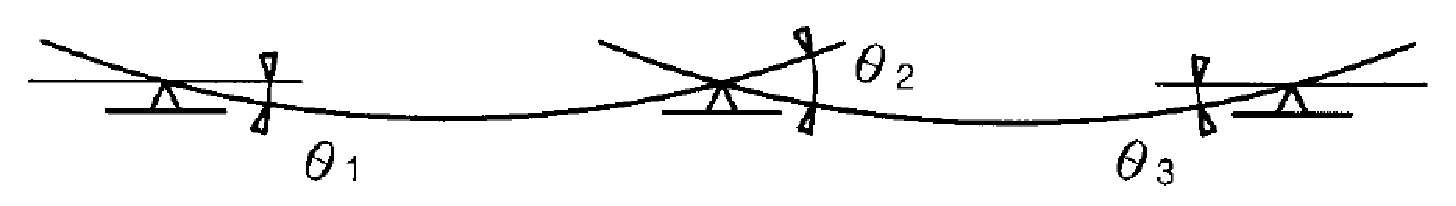
\includegraphics[width=0.8\textwidth]{definitionangularrotations.pdf}
% 	\caption{Definition of anular rotations at the end of the decks. Extracted from \cite[Figure A2.2]{1990a2}}
% 	\label{fig:difinitionangularrotations}
% \end{figure}

\subsubsection{Transverse deformations and vibrations}\label{sec:Transverse-deformations-and-vibrations}
\cite[A2.4.4.2.4]{1990a2}  proposed that transverse deformation and vibration of the deck shall be checked for characteristic combinations of Load Model 71 and SW/0 as appropriate multiplied by the dynamic factor $\phi$ and $\alpha$ (or real train with the relevant dynamic factor if appropriate), wind loads, nosing force, centrifugal forces in accordance with \cite[6]{EC12} and the effect of a transverse temperature differential across the bridge.

The transverse deflection $ \delta_h $ at the top of the deck should be limited to ensure:

\begin{enumerate}
	\item a horizontal angle of rotation of the end of a deck about a vertical axis not greater than the values given in Table.~\ref{tab:maximumhorizontalrotation} , or
	\item the change of radius of the track across a deck is not greater than the values in Table.~\ref{tab:maximumhorizontalrotation} , or
	\item at the end of a deck the differential transverse deflection between the deck and adjacent track formation or between adjacent decks does not exceed the specified value
\end{enumerate}

\begin{table}[h]
	\centering
	\begin{tabularx}{0.8\textwidth}{cXcc}
	\hline
	Speed range V(km/h) & Maximum horizontal rotation(radian) & \multicolumn{2}{c}{Maximum change of radius of curvature}\\
	& & Single deck & Multi-deck bridge\\
	\hline
	$ V\leq 120 $ & $ \alpha_1 $ & $ r_1 $ & $ r_4 $ \\
	$ 120\leq V \leq 200 $ & $\alpha_2 $ & $r_2$ & $ r_5 $ \\
	$V>200$ & $ \alpha_3 $ & $r_3$ & $r_6$\\
	\hline
	\end{tabularx}
	\\
	NOTE 1 The change of the radius of curvature may be determined using:
			$$ r = \frac{L^2}{8 \delta_h}$$
			
	NOTE 2 The transverse deformation includes the deformation of the bridge deck and the substructure(including piers, piles and foundations).
			
	NOTE 3 The values for the set of $\alpha_i$ and $r_i$ may be defined in the National Annex. The recommended values are:
			
	$ \alpha_1 = 0.0035$; $\alpha_2=0.0020$; $\alpha_3=0.0015$;
			
	$ r_1  =1700$; $r_2=6000$; $r_3=14000$;
			
	$ r_4 = 3500$; $r_5 = 9500$; $ r_6 = 17500$
	
	\caption{Maxiumum horizontal rotation and maximum change of radius of curvature}
	\label{tab:maximumhorizontalrotation}
\end{table}

\textbf{The first natural frequency of lateral vibration of a span should not be less than $f_{h0}$. The value for $f_{h0}$ may be defined in the National Annex. The recommended value is: $f_{h0}=1.2 Hz$}

Evidence of \cite{d181} is the origin of \cite[A.2.4.4.2.4(3)]{EC12} is found in \cite[p4.2: Lateral Frequencies]{d181}:

\begin{quote}
In order to avoid the phenomena of lateral resonance in vehicles, the first natural frequency of lateral vibration of the span $f_{lt}$ such that:

$$f_{lt} \geq 1.2Hz$$

\end{quote}

Until now there's no further instructions in EN1991-2 for bridges which can not pass 1.2Hz criterion. However, for bridges longer than 100 meters, they are almost guaranteed to fail 1.2Hz criterion. In order to solve this problem, a detailed analysis is conducted in Sec.\ref{sec:1.2criterion329}

\section{Conclusion}

There are altogether two regulations regarding lateral dynamics of railway bridges in EN1991-2. They are:

\begin{enumerate}
	\item Nosing force(action)
	\item 1.2Hz criterion 
\end{enumerate}

These two regulations have the same background documents: D181 report series. The analysis of D181 report series will be carried out in following chapter.

% \paragraph{Longitudinal displacements}
% For rails on the bridge and on the adjacent abutment, the permissible additional rail stresses due to the combined response of the structure and the track, due to variable actions, should be limited to the following design values:

% \begin{enumerate}
% 	\item Compression: $72KN/mm^2$
% 	\item Tension: $92KN/mm^2$
% \end{enumerate}

% \begin{figure}[p]
% 	\centering
% 	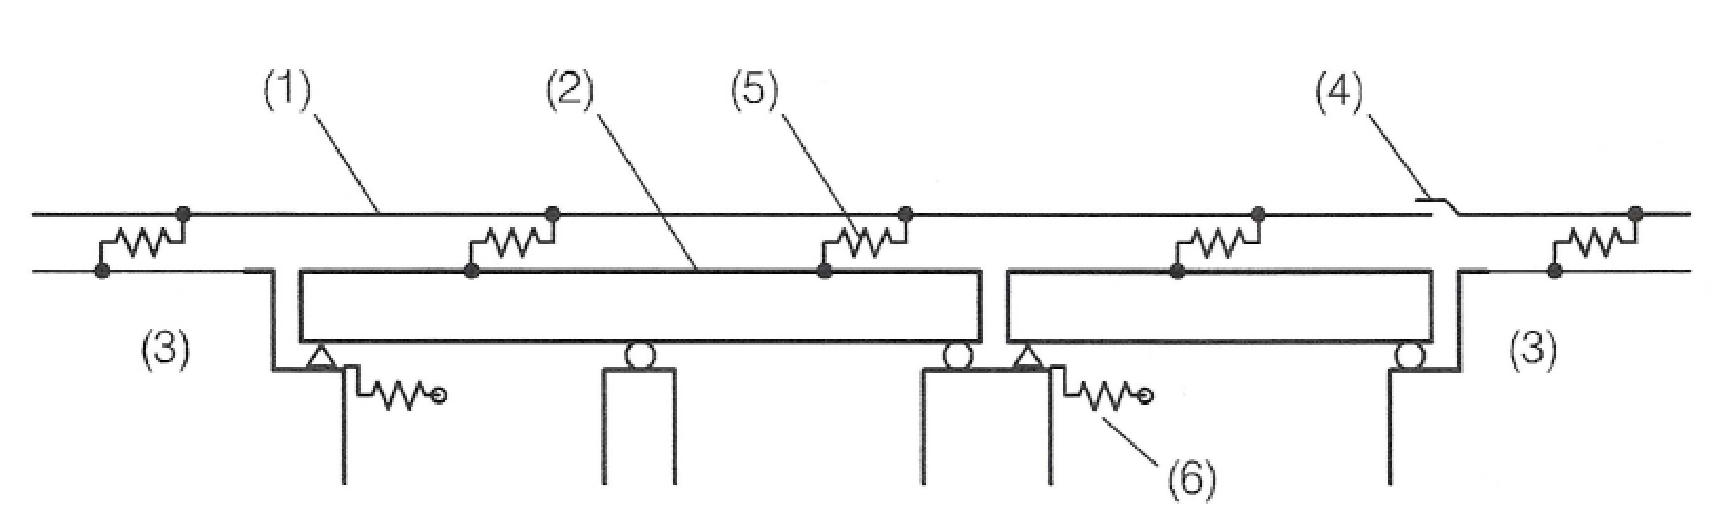
\includegraphics[width=0.8\textwidth]{modeltrackstructure.pdf}
% 	\caption{Model of a track/structure system. Extracted from \cite[Figure 6.19]{EC12}}
% 	\label{fig:modeltrackstructure}
% \end{figure}

% \begin{figure}[p]
% 	\centering
% 	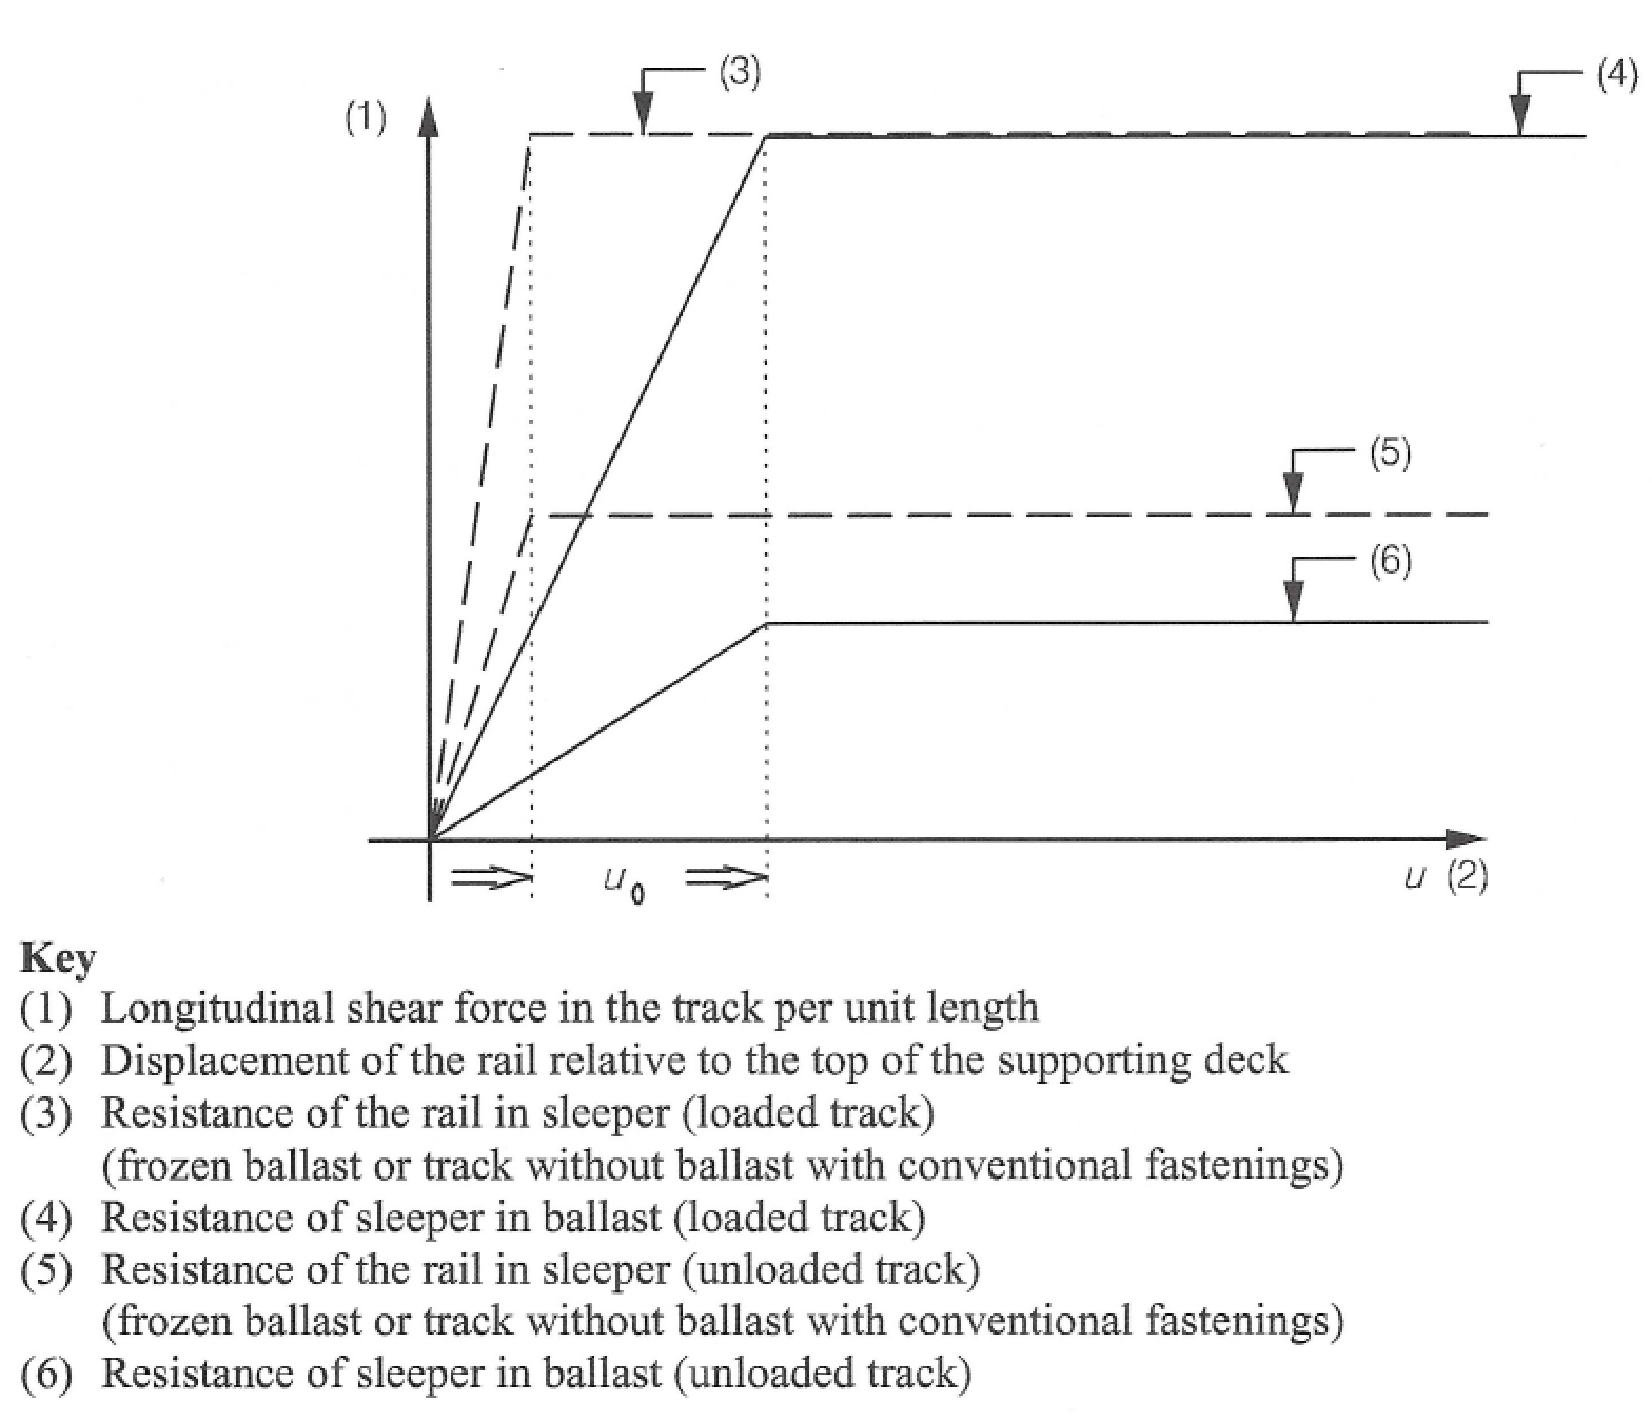
\includegraphics[width=0.8\textwidth]{variationlongitudinalshearforce.pdf}
% 	\caption{Variation of longitudinal shear force with longitudinal track displacement for one track. Extracted from \cite[Figure 6.20]{EC12}}
% 	\label{fig:variationlongitudinalshearforce}
% \end{figure}

% When determining the combined response of track and structure to traction and braking forces, these forces should not be applied on the adjacent embankment unless a complete analysis is carried out considering the approach, passage over and departure from the bridge of rail traffic on the adjacent embankments to evaluate the most adverse load effects.

% For the determination of load effects in the combined track/structure system a model based upon Figure\ref{fig:modeltrackstructure} may be used where the longitudinal load/displacement behaviour of the track or rail supports may be represented by the relationship shown in Figure.\ref{fig:variationlongitudinalshearforce}.

% Model in Figure\ref{fig:modeltrackstructure} is very important to evaluate the security of the track structure and not the structural security. High track deformations can lead to unfavourable effects for the structure and for vehicles when these are crossing the bridge.

% \subsubsection{Serviceability limit states - passenger comfort}

% For these type of verifications \cite{1990a2} defines the limiting values for the maximum vertical deflection for passenger comfort, as following:

% \begin{enumerate}
% 	\item Comfort criteria
% 	\item Deflection criteria for checking passenger comfort
% 	\item Requirements for a dynamic vehicle/bridge interaction analysis for checking passenger comfort
% \end{enumerate}

% Passenger comfort depends on the vertical accelerations, $b_v$, inside the coach. These levels of comfort limiting values for the vertical accelerations are presented in Table.\ref{recommendedaccelerationsvalues}

% \begin{table}[h]
% 	\centering
% 	\begin{tabular}{cc}
% 		\hline
% 		Very good & $1.0m/s^2$ \\
% 		Good & $1.3 m/s^2$ \\
% 		Acceptable & $2.0m/s^2$\\
% 		\hline
% 	\end{tabular}
% 	\caption{Recommended accelerations values to ensure the respective levels of comfort. Extracted from \cite[Table A 2.9]{1990a2}.}
% 	\label{recommendedaccelerationsvalues}
% \end{table}

% \begin{figure}[h]
% 	\centering
% 	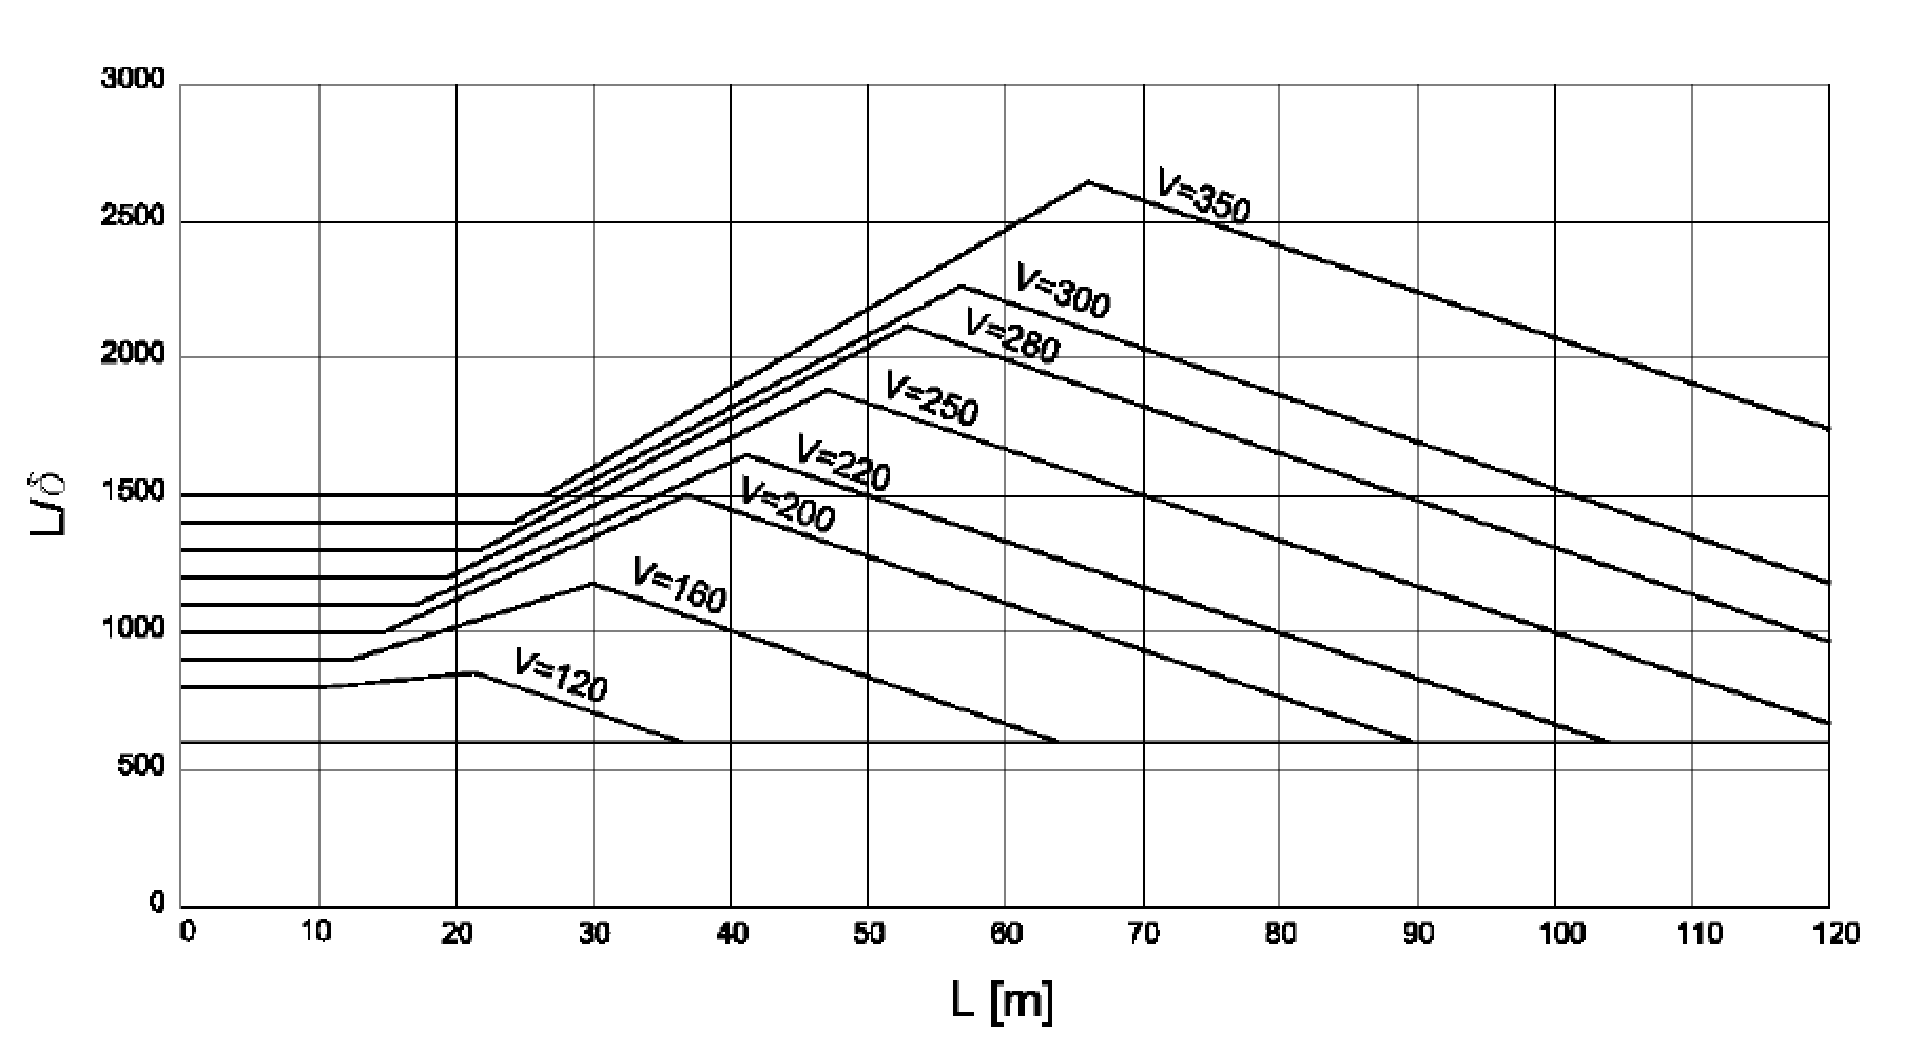
\includegraphics[width=0.8\textwidth]{recommendedlevelofcomfort.pdf}
% 	\caption{Maximum permissible vertical deflection $\delta$ for railway bridges with 3 or more successive simply supported spans corresponding to a permissible vertical acceleration of $b_v=1m/s^2$ in a coach for speed $V$[km/h]. Extracted from \cite[Figure A2.3]{1990a2}}
% 	\label{fig:recommendedlevelofcomfort}
% \end{figure}

% In order to limit vertical vehicle acceleration, being the limits defined in Table\ref{recommendedaccelerationsvalues},vertical displacements should be less than the maximum permissible vertical deflection, $\delta$, obtained from Figure\ref{fig:recommendedlevelofcomfort}. These values are expressed in function of the span length $L$[m], and train speed $V$[km/h], which is valid only for railway bridges with three or more successive simply supported spans. Alternatively these accelerations can be determined considering the vehicle-structure interaction dynamic analysis.

% Additionally, the limiting values of $L/\delta$, defined in Figure\ref{fig:recommendedlevelofcomfort} are given for $b_v=1.0m/s^2$.

% Vertical deflections should be determined with the LM 71 model multiplied by the factor $\phi$ and adopting $\alpha=1$, being only one track loaded for the case of bridges with two or more tracks.

% \subsection{Principal supplementary checks}
% \subsubsection{Verification of maximum peak deck acceleration along each track}
% \subsubsection{Verification of whether the calculated load effects from high-speed rail traffic, including HSLM on high-speed interoperable routes, are greater than those of normal rail traffic loading(LM71''+''SW/0)}
% \subsubsection{Additional verification for fatigue where dynamic analysis is required}
% \subsubsection{Verification of limiting values for the maximum vertical deflection for passenger comfort}

% \subsection{Diagram of general procedures}
% By summarizing Eurocode several steps of calculation are extracted as following, arranged in chronological order.

% \begin{enumerate}
% 	\item  Follow the conceptual check to avoid unsafe designs
% 	\item  Follow the logic diagram in Figure~\ref{fig:logicdiagram} to check whether dynamic analyses are required 
% 	\item  Find the appropriate train models, including 
% 	\begin{enumerate}
% 		\item-Hypotheses relating to rolling stock
% 		\item-Rolling stock for interoperability
% 		\item-Load models HSLM
% 		\item-Load distribution
% 		\item-Load combinations and partial factors
% 		\item-Train speeds to be considered
% 	\end{enumerate}
% 	\item Perform the static analyses
% 	\item  Examine bridge parameters, including
% 		\begin{enumerate}
% 			\item-Structural damping
% 			\item-Mass of the bridge
% 			\item-Stiffness of the bridge
% 		\end{enumerate}
% 	\item Perform the dynamic analyses
% 	\item  Principal supplementary design checks, including
% 	\begin{enumerate}
% 		\item-Verification of maximum peak deck acceleration along each track
% 		\item-Verification of whether the calculated load effects from high-speed rail traffic, including HSLM on high-speed interoperable routes, are greater than those of normal rail traffic loading(LM71''+''SW/0)
% 		\item-Additional verification for fatigue where dynamic analysis is required
% 		\item-Verification of limiting values for the maximum vertical deflection for passenger comfort
% 	\end{enumerate}
% 	\item The results of the dynamic analysis shall be compared with the results of the static
% analysis multiplied by the dynamic factor $\varPhi$ in 6.4.5 The most unfavourable values of the load effects shall be used. 
% \end{enumerate}

% \section{Dynamic analysing methods}\label{sec:dynamic-analysing-methods}
% There are several dynamic analysing methods developed in Europe over time since Eurocodes don't specify what method to be used during dynamic analysing. These methods differ from each other in the level of calculation complexity. For example, Dynamic train signature method is a good solution for simple structures with well-known train types since it cost less time and effort. On the other hand, Train-vehicle method is an inevitable process for some complicated bridge structures thanks to its wide applicability. However, generally, Train-vehicle method is much more time and money consuming. In following paragraphs, some state-of-art dynamic analysing methods will be reviewed.


% \subsection{Method based on impact factor}

% \subsection{Method based on dynamic train signature}
% As mentioned in \cite[A.4.3]{uic}, the dynamic signature of a train is obtained by breaking down the load diagram of a train in Fourier series and by extrapolating it to the natural modes. It represents the dynamic excitation features of the train and is independent of the characteristics of the structure. The signature depends on axle spacing and loads only. However, newly developed Train dynamic signature method like LIR method takes structure characteristics into account, giving more applicable solutions for specific bridge projects.

% Train dynamic signature is a useful method of producing quick analyses on resonance characteristics of the vehicle-bridge systems. The method is especially effective for simple bridge structures.

% \subsubsection{DER method}

% DER = Decomposition of the Resonance Excitation

% The development used in DER method begins from the analysis of the frequency of excitation produced by a train of moving loads. This method is based in the following assumptions:

% \begin{enumerate} [-]
% 	\item Applicable only on statistically determined bridges
% 	\item For the analysis of statistically determined bridges, is considered that the dynamic response is significantly represented by the first mode of vibration
% \end{enumerate}

% The development of the method is summarised as follows:

% \begin{enumerate}
% 	\item Reduce the response of a statistically determinate beam to a single degree of freeedom system
% 	\item Decomposition of the dynamic response of the bridge, in Fourier series;
% 	\item Consideration of the term which corresponds to the condition of resonance frequencies.
% \end{enumerate}

% The maximum accelerations at the midspan of the beam for a certain speed, is given as follows:

% \begin{equation}
% 	\ddot{y}(t)\leq C_t\cdot A(L/\lambda)\cdot G(\lambda)
% \end{equation}

% where the first factor is a constant that depends from bridge characteristics:

% \begin{equation}
% 	C_t=\dfrac{8\pi f_0^2}{K}=\dfrac{4}{\rho\pi L}  
% \end{equation}

% The second factor is a function called dynamic influence line:

% \begin{equation}
% 	A(L/\lambda )= \bigg\vert\dfrac{\cos (\pi L/\lambda)}{(2L/\lambda)^2-1} \bigg\vert
% \end{equation}

% and the third factor represents the train dynamic signature, defined as follows:

% \begin{equation}
% 	G(\lambda)=\sqrt{[\sum_{k=1}^N F_k\cos(\dfrac{2\pi x_k}{\lambda})]^2+[\sum_{k=1}^N F_k \sin(\dfrac{2\pi x_k}{\lambda})]^2}\cdot (1-e^{-2\pi \xi \dfrac{x_N}{\lambda}})\cdot \dfrac{L}{\xi x_N}
% \end{equation}

% \subsubsection{LIR method}
% LIR method is based on residual influence line. It is applicable only on statistically determined bridges, too. The solution of the displacements and accelerations in the midspan, of the simply supported beam, is developed by \citeauthor{dominguez2001dinamica}. The solution is given as follows:

% \begin{equation}
% 	\centering
% 	y_{max}=C_{desp}\cdot A(r) \cdot G(\lambda)
% \end{equation}

% \begin{equation}
% 	\ddot{y}_{max}=C_{acel}\cdot A(r) \cdot G(\lambda)
% \end{equation}

% with,

% \begin{equation}
% 	C_{desp} = \frac{1}{M\omega_0^2},
% 	C_{acel} = \frac{1}{M}
% \end{equation}

% The factor $ A(r) $ is the dynamic influence line, give as:

% \begin{equation}
% 	A(r)=\frac{r}{1-r^2}\sqrt{e^{-2\xi \frac{\pi}{r}}+1+2\cos (\frac{\pi}{r})e^{-2\xi \frac{\pi}{r}}}
% \end{equation}

% with $ r=\lambda/2L $.

% $G(\lambda)$ is named train dynamic signature, depending from train characteristics and from the damping coefficient of the structure, give as follows:

% \begin{equation}
% \end{equation}

% To make $G(\lambda)$ representative for the maximum response, maximum value of $G(\lambda)$ for each different subtrain is considered the value of $G(\lambda)$

% \begin{equation}
% 	G(\lambda) = \max_{i=1}^{N} \sqrt{[\sum_{x_1}^{x_i}F_i\cos (2\pi \delta_i) e^{-2\pi \xi \delta_i}]^2+[\sum_{x_1}^{x_i}F_i \sin (2\pi \delta_i) e^{-2\pi \xi \delta_i}]^2}
% \end{equation}

% \begin{figure}[h]
% 	\centering
% 	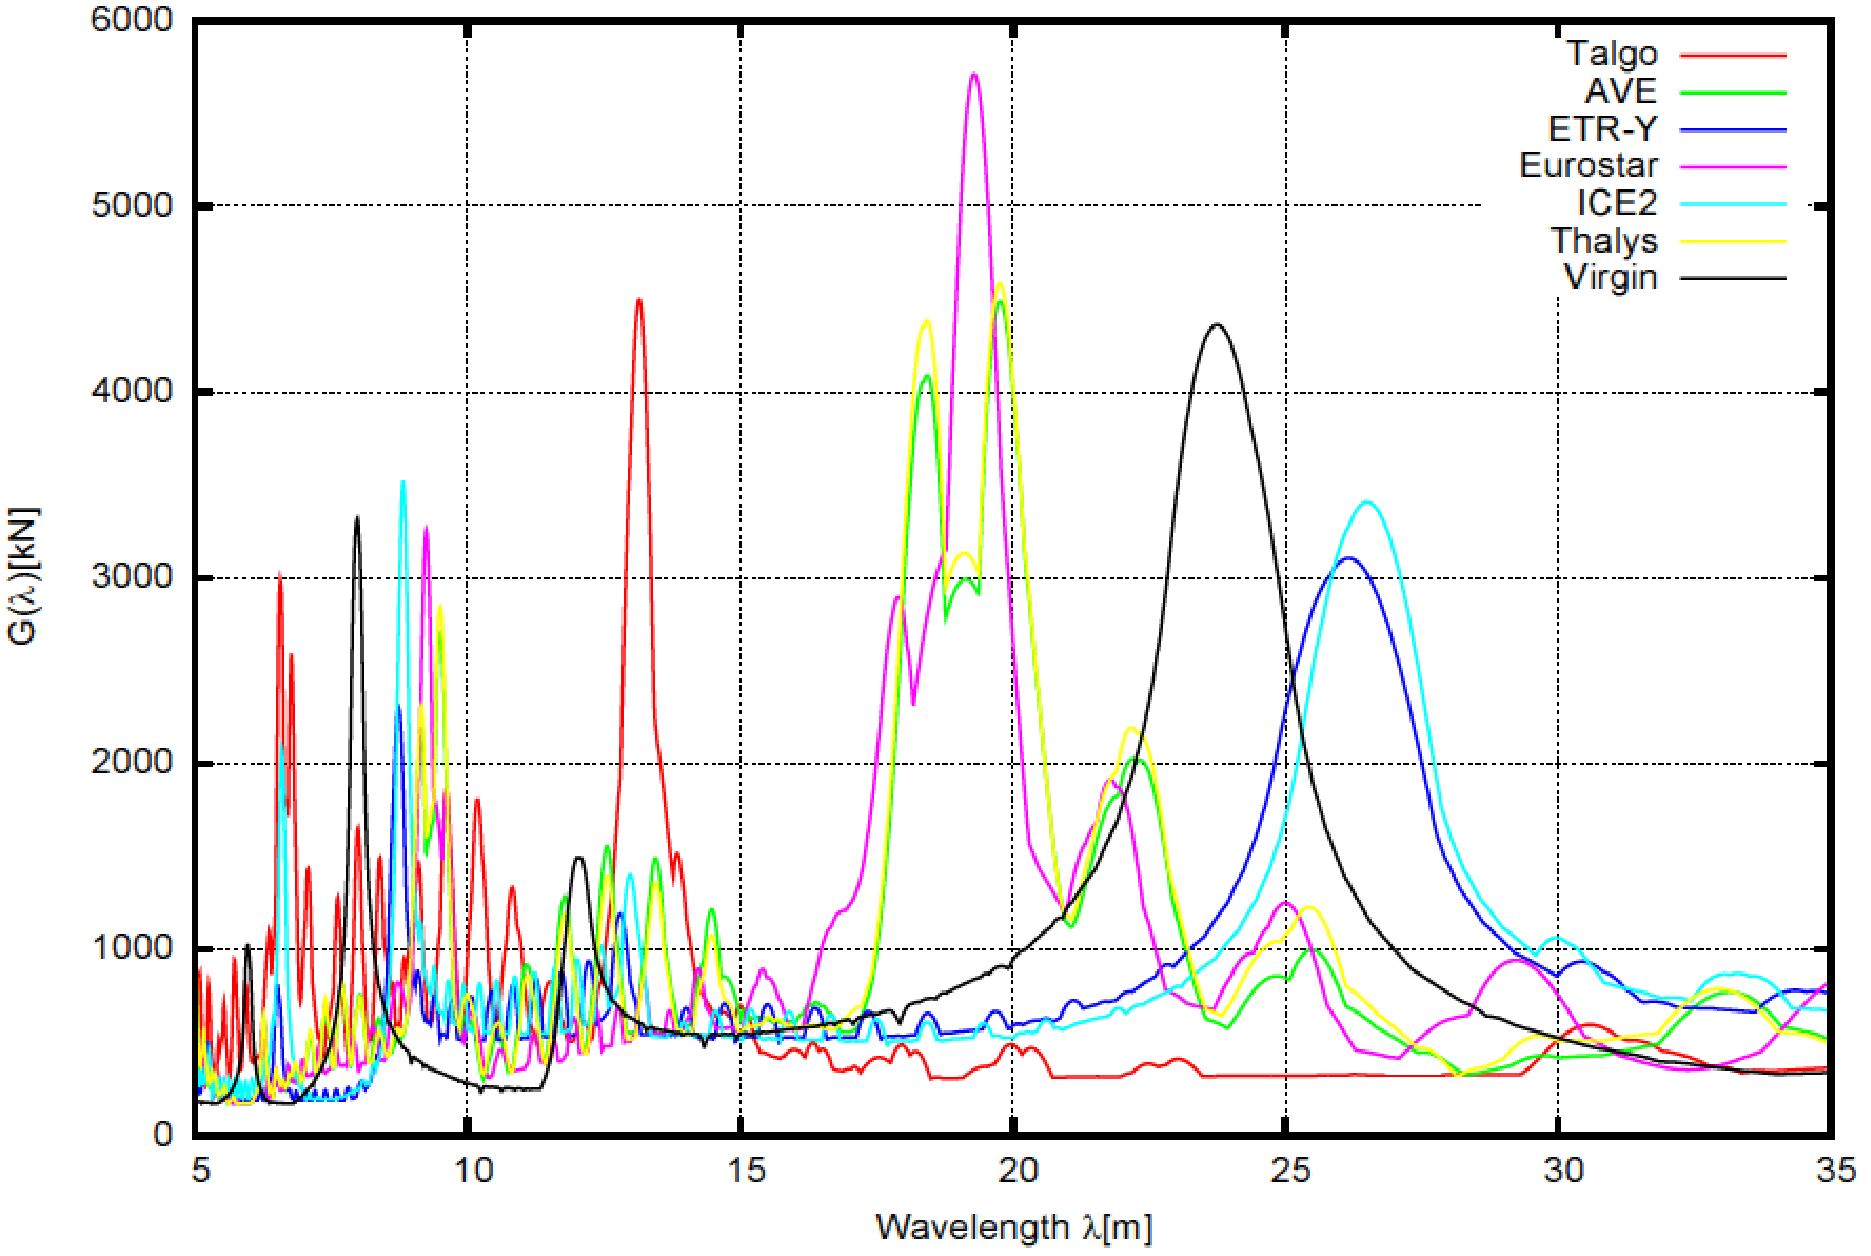
\includegraphics[width=0.6\textwidth]{trainsig.pdf}
% 	\caption{Train dynamic signatures for the seven real trains, considering a damping value of $\xi = 0.00$. Extracted from \cite[Figure 2.20]{da2007dynamic}}
% 	\label{trainsig}
% \end{figure}

% \subsection{Methods based on finite element models}
% Finite element methods are the most applicable methods available. The methods are based on direct time integration.

% \subsubsection{Direct time integration methods}
% General equation of motion for a SDOF system can be given in following form:

% \begin{equation}
% 	\boldsymbol{M\ddot{d}}+\boldsymbol{C\dot{d}}+\boldsymbol{Kd}=\boldsymbol{f}(t)
% \end{equation}

% where $\boldsymbol{M}$ is the mass matrix, $ \boldsymbol{c} $ is the damping matrix, $ \boldsymbol{K} $ is the stiffness matrix, $ \boldsymbol{f}(t) $ is the vector of external loads and $ \boldsymbol{d} $ the unknown vector of nodal displacements. 

% Direct time integration method is the principle of finite element models. Due to the expected huge amount of calculation, computers are used to process time integration calculations. Thanks to the reliability and efficiency of computers, there are more and more project done with the help of computer FEM software nowadays.

% \subsubsection{Modelling a train of moving loads}
% The method of modelling spatial moving loads in FEM software is applying load histories in each convenient node. At a certain time-step, a load F, whose magnitude depending linearly on the distance from the axle to the node, is assigned to each node if the load axis is above an element that contains the node. The procedure is outlined in Figure.\ref{fig:movingloads}.

% \begin{figure}[h]
% 	\centering
% 	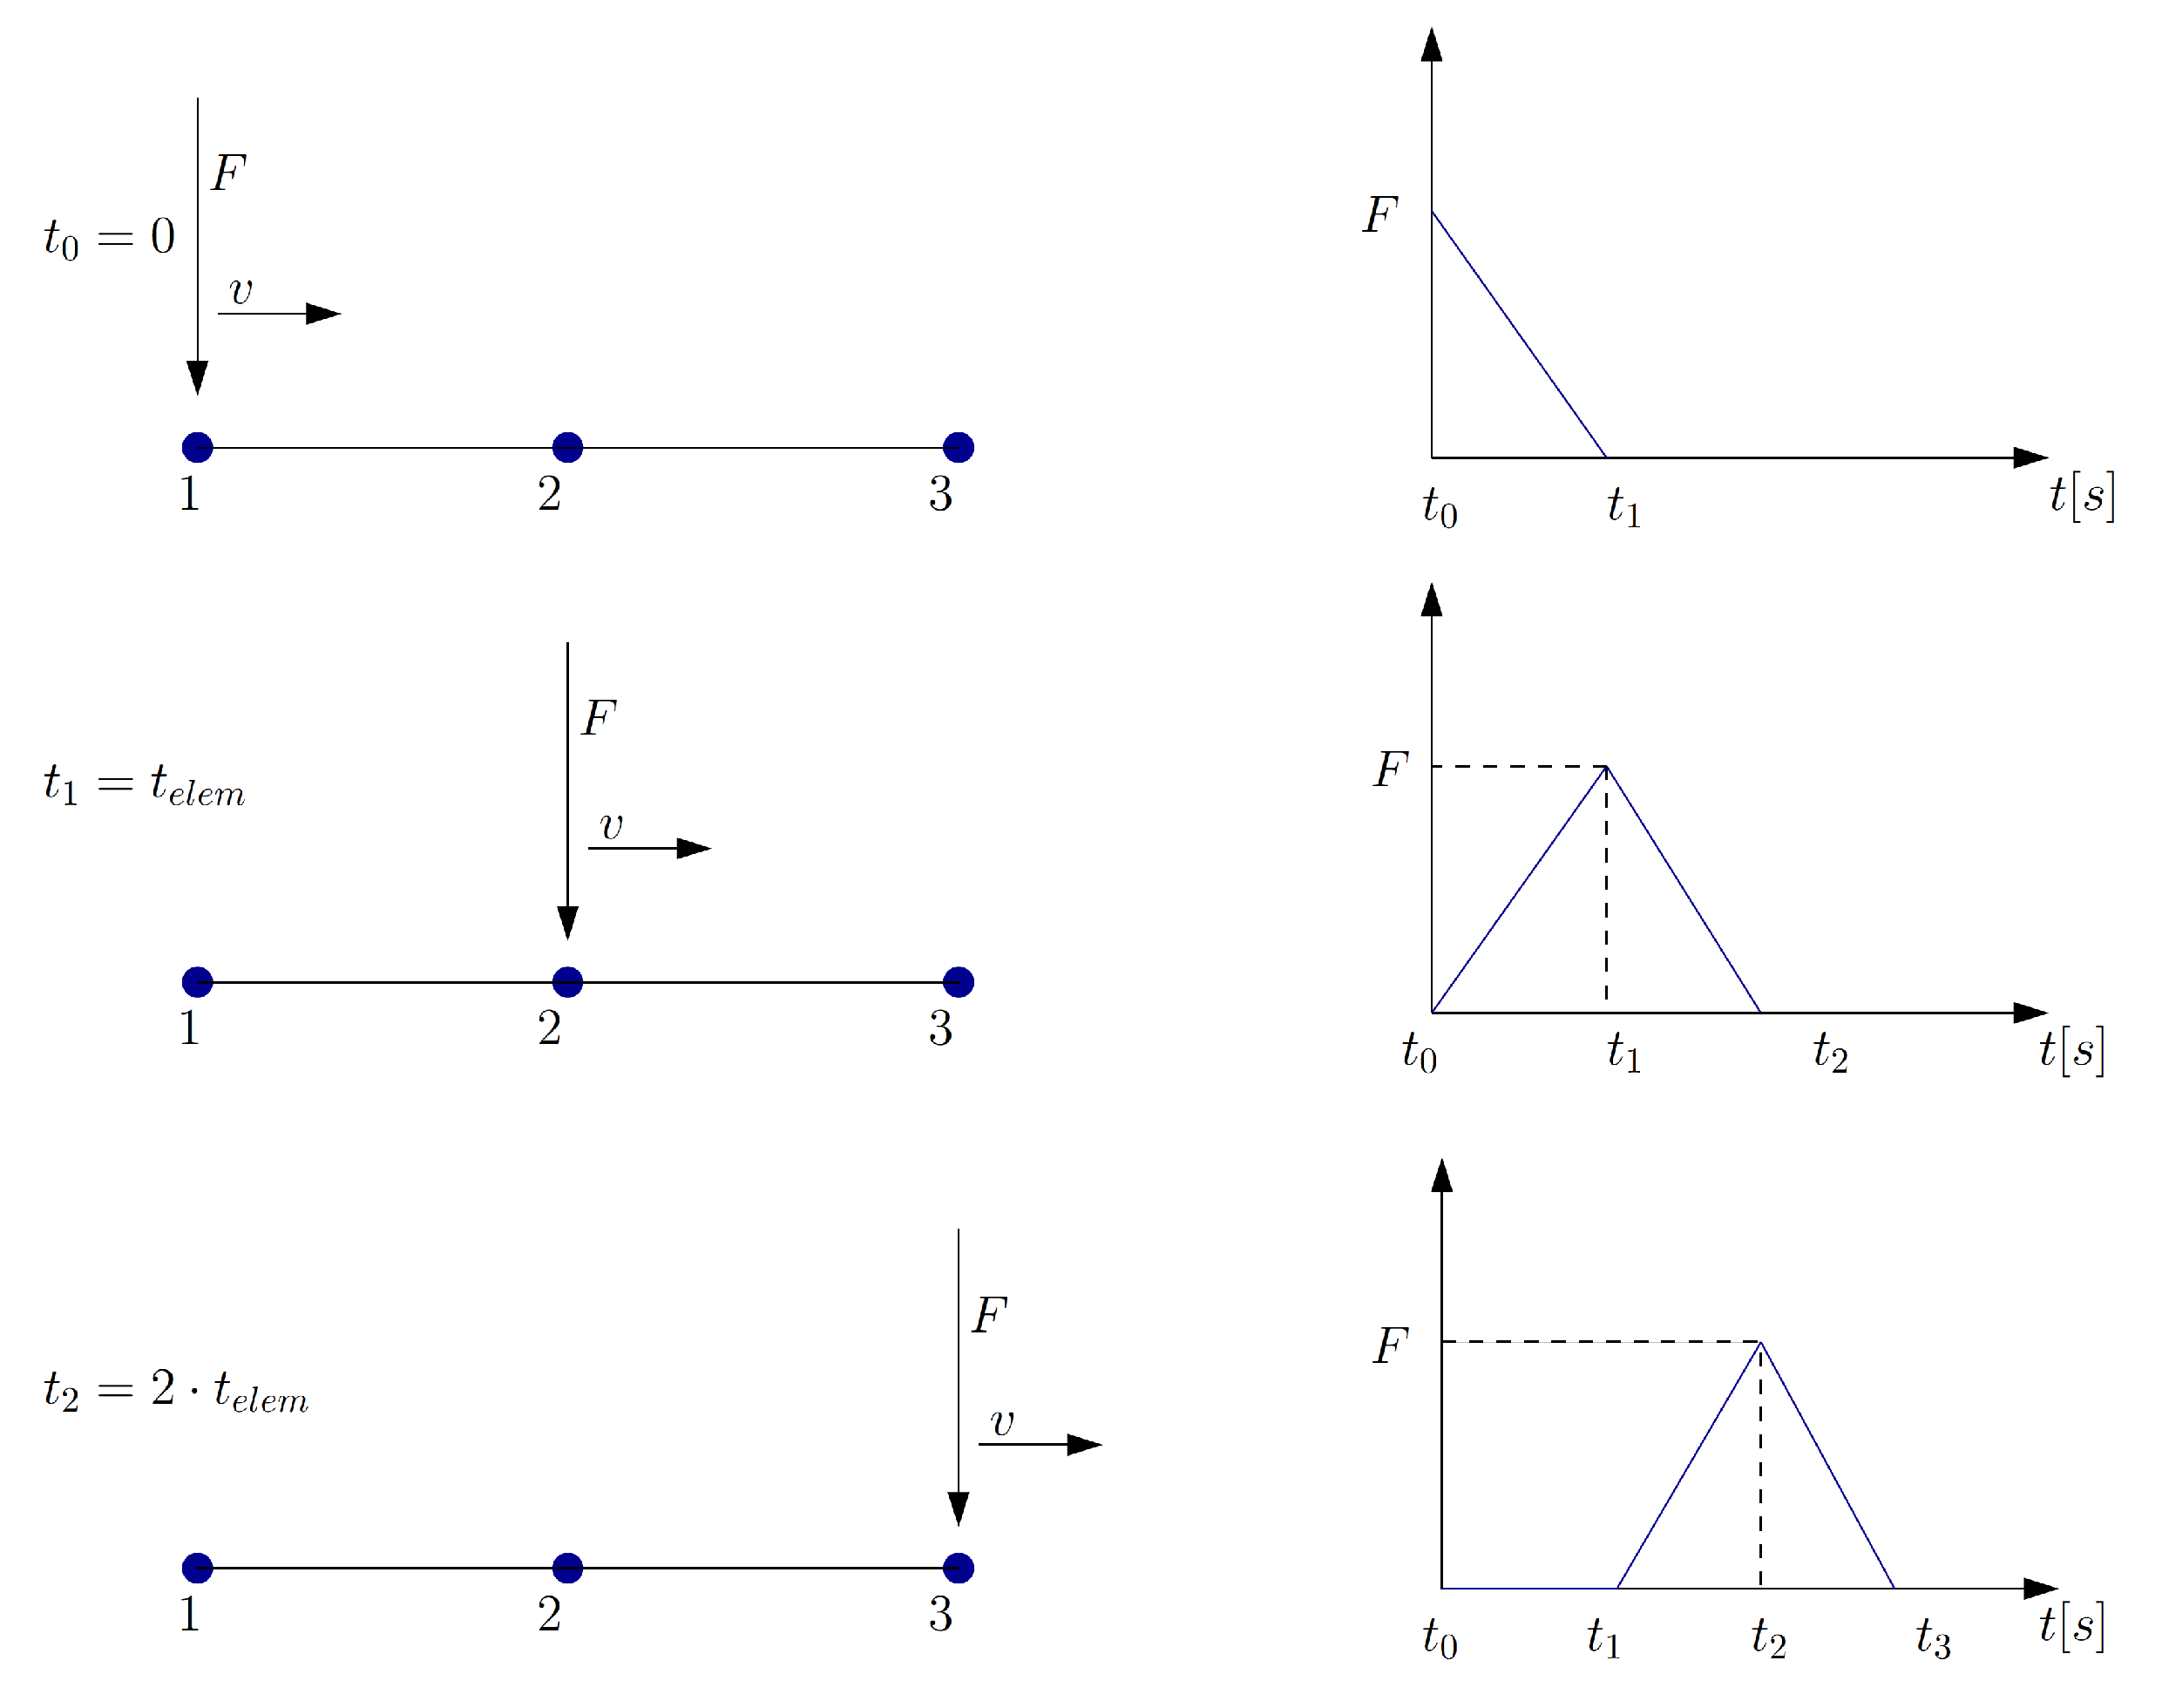
\includegraphics[width=0.8\textwidth]{movingloads.pdf}
% 	\caption{Nodal force time history definition for a single moving load $F$, with speed $v$. Extracted from \cite[Figure 2.15]{da2007dynamic}}
% 	\label{fig:movingloads}
% \end{figure}

% \subsection{Analytical methods based on modal analysis}
% Modal analysis is the study of the dynamic properties of structures under vibrational excitation. Applied on railway bridge structures, the analysis can be simple if the bridge is modelled as a simply supported beam.



% \subsection{Method based on vehicle-Structure interaction dynamic analysis}\label{sec:tds}
% Different from point load models, vehicle-structure models takes suspension systems of train vehicles into account, providing associations between train carriage and structure. Impact of suspension system vibration on bridge structure can be neglected when the span of the bridge is comparably small since there's little chance for suspension system and bridge to resonant. As the span of bridges increase, the first vertical/transverse natural frequency of bridge can decrease into the natural frequency range of train suspension system. This means long-span bridges can resonant with train suspension system. To study the effects related to train suspension system, vehicle-structure interaction method is developed. 

% A general model for a conventional coach on two bogies are shown in Figure.\ref{fig:vehicle-structure}, including the stiffness and damping $(K_P,c_P)$ of the primary suspension of each axle, the secondary suspension of the bogies $(K_s,c_s)$, the unsprung mass of the wheels $(M_w)$, the bogies $(M_b, J_b)$, and the vehicle body $(M,J)$. Similar models may be developed for articulated or regular trains.

% \begin{figure}[h]
% 	\centering
% 	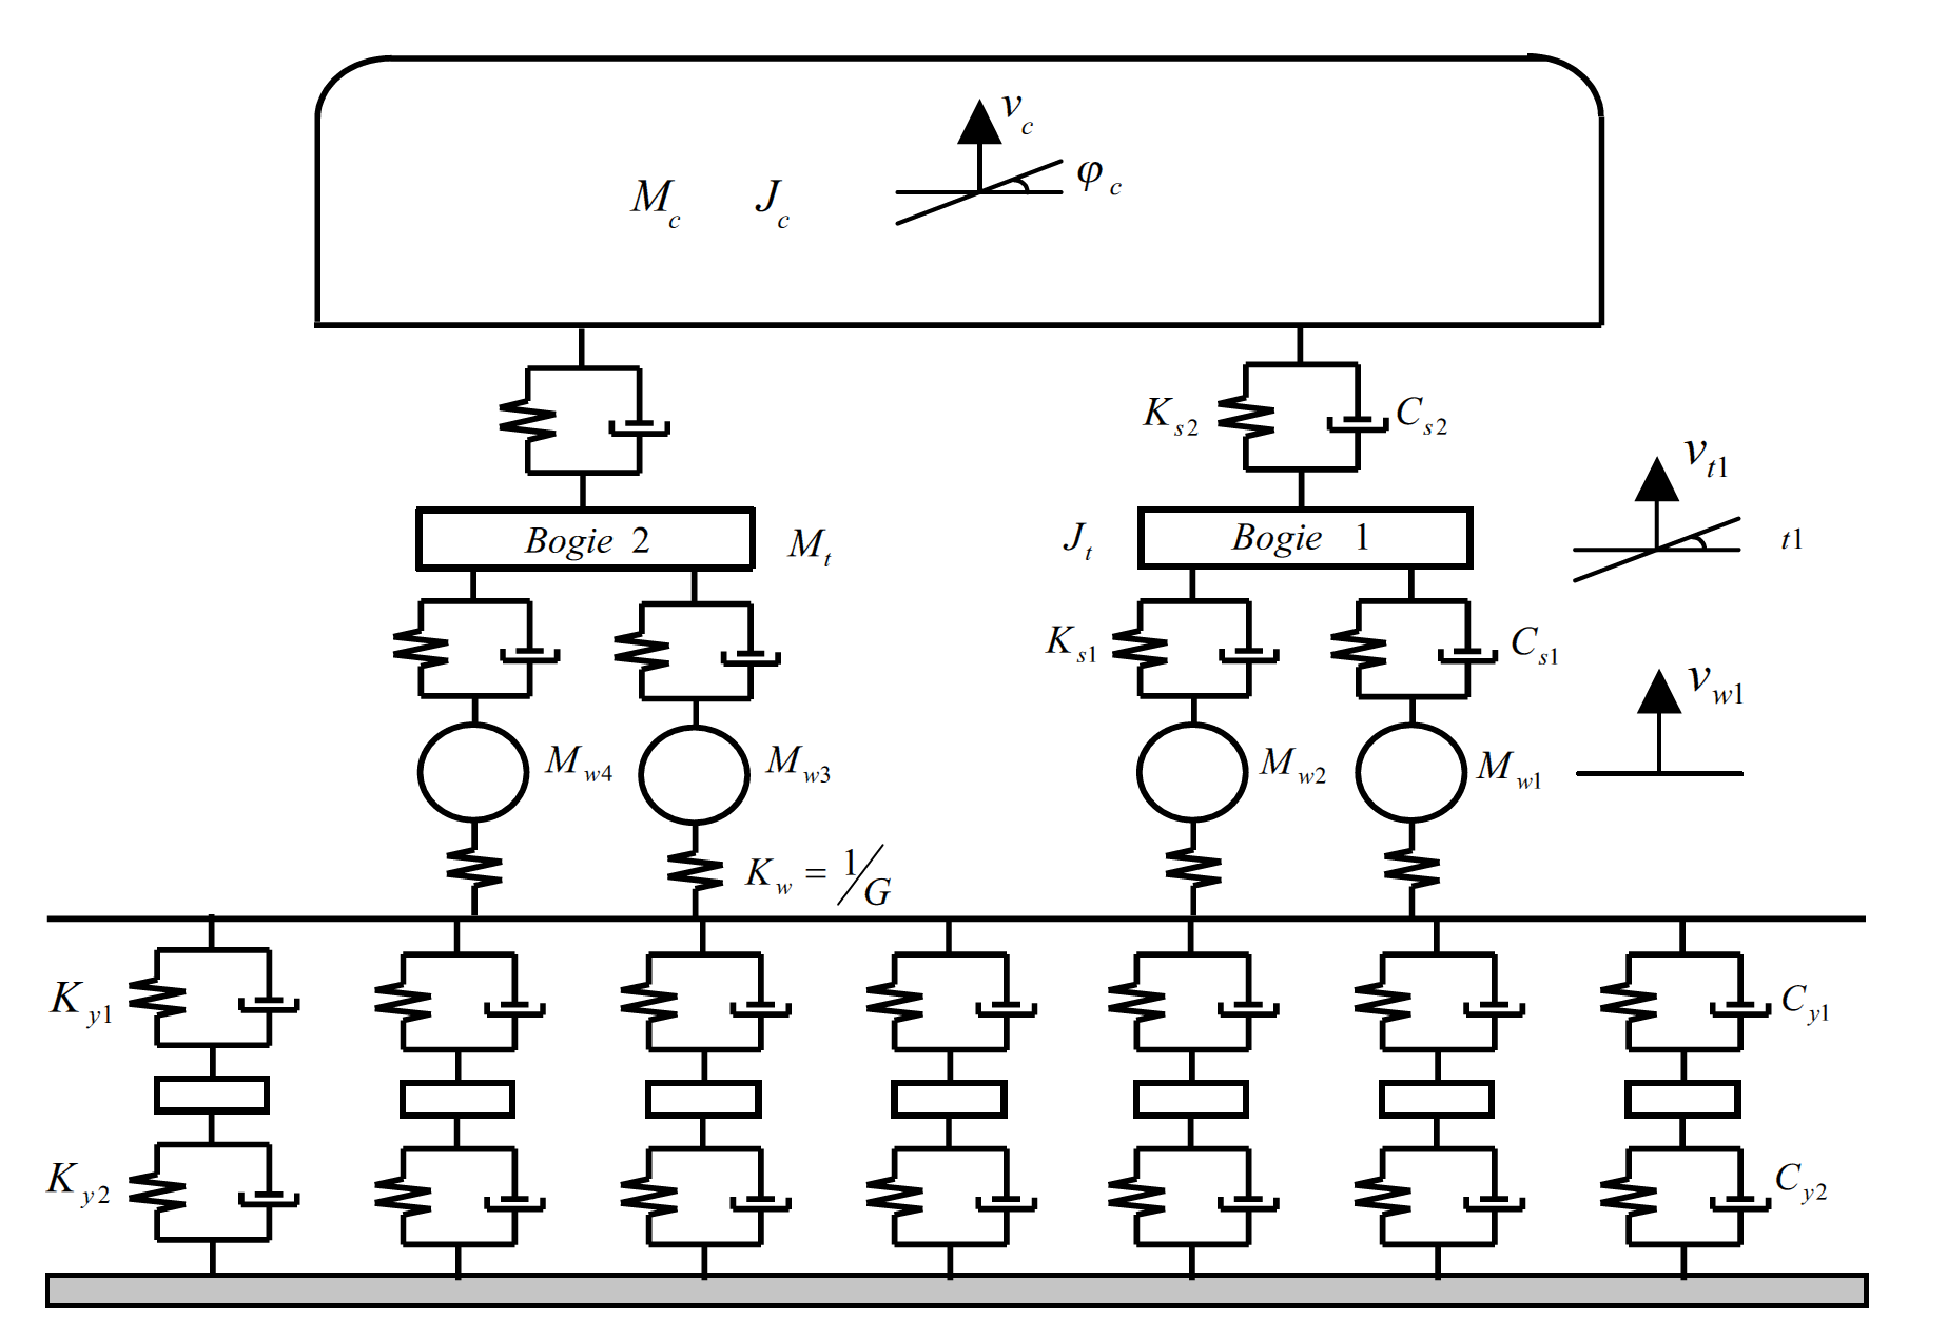
\includegraphics[width=0.8\textwidth]{vehicle-structure.pdf}
% 	\caption{Model for analysis of vehicle-structure system. Extracted from \cite[Figure 12]{lei2002analyses}}
% 	\label{fig:vehicle-structure}
% \end{figure}

% Sometimes more simplified model , represented by one mass, one spring and one damper per bogie can be considered, depending on the purpose of the analysis. See Figure\ref{fig:simplified-vehicle-structure} for example.

% \begin{figure}[h]
% 	\centering
% 	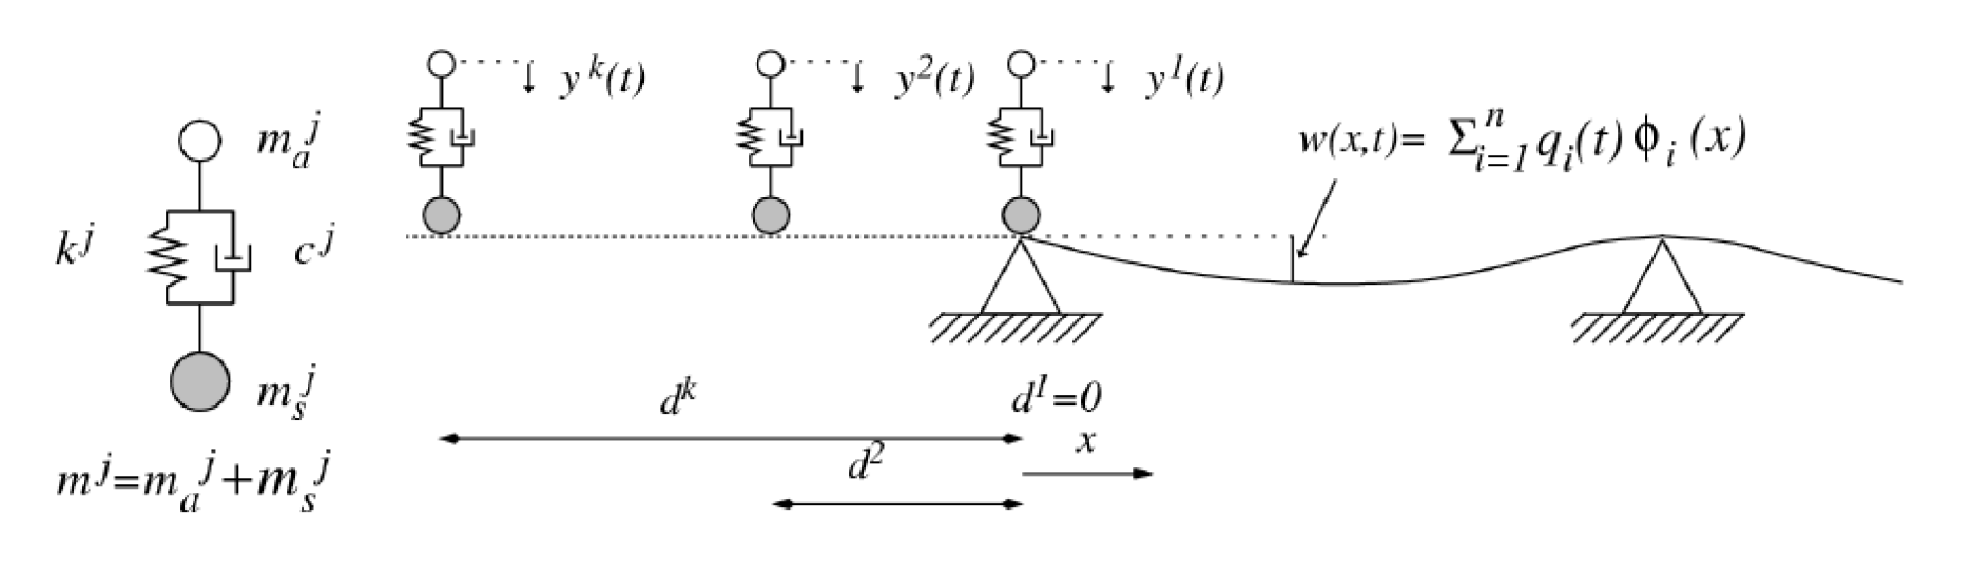
\includegraphics[width=0.8\textwidth]{simplifiedvehiclestructure.pdf}
% 	\caption{Load train with vehicle-bridge interaction: simplified interaction model and variables definition. Extracted from \cite[Figure15]{lei2002analyses}}
% 	\label{fig:simplified-vehicle-structure}
% \end{figure}


\chapter{Investigation of report series created by D181 Committee Group}


\section{Introduction}

D181 Committee Group is created by UIC, in order to investigate Lateral Forces on Railway Bridges. Some of the proposed criteria in reports created by this committee group are adopted by Eurocode Committee to created Eurocode 1991-2. The goal of this investigation is to summarize the research done by D181 report series and and give further conclusion.

The investigation will be done in following aspects:

\begin{enumerate}
    \item Investigation of DT329
    \item Investigation of RP6
    \item Conclusion of D181 report series
\end{enumerate}

\subsection{Structure of report series}

Reports involved in the series are listed below in the order of publishing time:

\begin{enumerate}
    \item RP 1: Summaries of national standards and literature survey
    \item RP 2: Submitted programs and example of application
    \item RP 3: Dynamic measurements on the steel bridge over the Brenta river on the MilanVenice line at 234 + 0.963 km
    \item RP 4: Dynamic measurements on steel bridges over the Váh river by Sala on the MarcheggSzob line at 117 748 km
    \item DT 312: Etude de l'influence de la fréquence du filtre sur les valeurs mesurées des forces verticales et latérales sur les rails
    \item RP 5: Dynamic measurements on the metal arched bridge on PKP
    \item DT 313: Analyse des déformations latérales d'un pont souple (cas du PONT de LIXHE) Ligne SNCB de TONGRESMONTZEN par J.J. REBER SBB Bau GD
    \item DT 329: Parametric study Part 1: Parametric study Initial phase (September 1994) Part 2: Parametric study Phase 2 (February 1995) Authors: L.T. James and G.A. Scott
    \item RP 6: Final Report
\end{enumerate}

In this thesis DT 329 and RP 6 are obtained and studied, but other reports in English version are not available to the researcher.

\subsection{Items of interests in report series}

\begin{enumerate}
    \item Resonance mechanisms studied. They are discussed in DT329. See Section.\ref{sec:resonance329}
    \item The proposed 1.2 Hz Criterion and its background. It is discussed in RP6. See Section.\ref{sec:1.2criterion329}
    \item  Lateral forces(Nosing force) on the bridges. See Section.\ref{sec:lateralforce329}
\end{enumerate}

\section{Investigation of DT329}
\subsection{Methodology of Parametric Research DT329}

The DT329 research was conducted in two phases. It is noted that all studies were done using VAMPIRE software. The reliability of simulation has been discussed and confirmed in previous reports. 

In the initial phase 11 sets of bridge parameters were selected for the simulation. 52 combinations of bridge parameters and train configurations were examined. The goal of the initial phase is to filter out most influencing parameters for bridge dynamics.

In the secondary phase, the influence of selected parameters were categorized into 3 cases. They include:
\begin{enumerate}
 \item the influence of multiple span bridges (viaducts)
 \item the influence of track quality
 \item the influence of stiffness/span/frequency on the resonant behaviour of the bridge
\end{enumerate}
They were studied by using the same simulation method used in initial research phase.




% For the initial phase, the dynamic lateral response to the passage of different train types were examined.

% The method of modelling bridge behaviour adopted is the Theory of Normal Modes. Each train is modelled as a series of masses interconnected by suspension components of known characteristic. Time-step integrations are then performed to simulate the passage of a train over the bridge model along a track sample, which extends beyond the bridge.

% Comparisons of measured bridge responses with VAMPIRE simulations of the bridges and trains involved were the subject of earlier studies for ERRI Committee D 181, the results being documented in reports RP 3, RP 4, and RP 5 of the Committee. Each vibration model was derived from finite element analysis of the bridge structure.

% The committee have selected eleven sets of bridge parameters to be subjected to a selection of lateral load conditions. Lateral loading is provided by three train types, each running at two speeds within their respective operational ranges, on track appropriate to the train type. The combinations selected for this phase are tabulated in Appendix 1. Since the bridge design parameters are necessarily general, finite element techniques for producing bridge vibration models are inappropriate; general transverse beam vibration theory is used instead.

% For the secondary phase, as part of ERRI(UIC) investigation of Lateral Forces on Railway Bridges, the ERRI D181 Committee have commissioned British Rail Research (BRR) to carry out a parametric study(DT329) using their VAMPIRE dynamics software. 

% The study has investigated the influence of key bridge parameters and of different train types on the lateral deflections and lateral forces exerted on the bridge. The study has been carried out in two phases.

% The first phase examined 52 combinations of bridge parameters and train configurations. This study showed that some of the input parameters had little influence on the dynamic behaviour of the bridge and that others had a significant influence. There were also some parameters which appeared to show resonant effects at particular values. The results were presented in the initial report (Reference [1], part 1 of this ERRl D 181/DT 329).

% From the results of the first phase of the study, the ERRI DI81 Committee were able to select the cases for the second part in order to concentrate on those parameters which had the largest influence on the behaviour of the bridge. The cases to be considered were divided into three categories. These investigated the influence of multiple span bridges (viaducts), the influence of track quality and the influence of stiffness/span/frequency on the resonant behaviour of the bridge.



% Focus is placed on secondary phase of study of DT329, since it consists research on resonance behaviour of the bridge.

\subsection{Modelling}\label{sec:modelling329}
A special version of VAMPIRE with bridge module implemented was used to run simulation analysis. 

For an overview of modelling setup in both research phases, see Figure \ref{fig:modelling overview}. Following paragraphs will give details of modelling.


\begin{figure}[h]
\centering
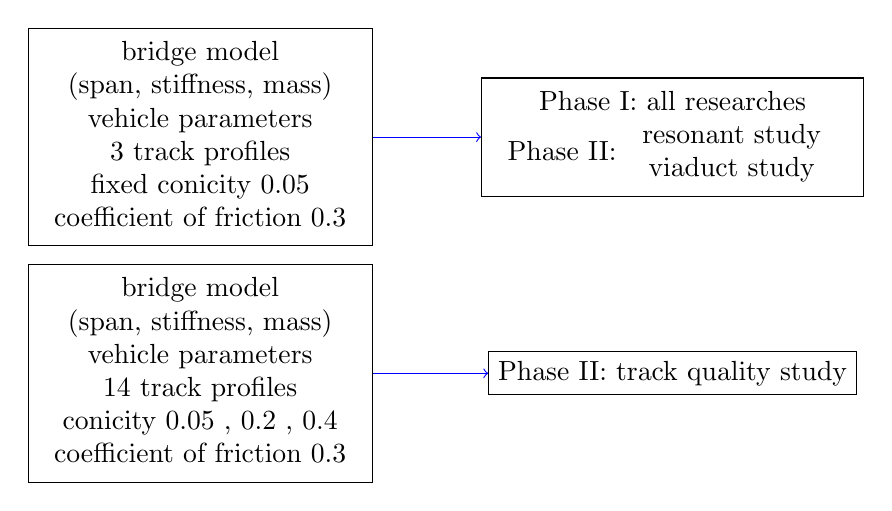
\begin{tikzpicture}

    \node[draw] (parameters) at (0,0) {
        \begin{tabular}{c}
            bridge model \\
            (span, stiffness, mass) \\
            vehicle parameters \\
            3 track profiles \\
            fixed conicity 0.05\\
            coefficient of friction 0.3 \\
        \end{tabular}
    };

    \node[draw] (phase I) at (6,0) {
        \begin{tabular}{c}
            Phase I: all researches \\
            Phase II: 
                \begin{tabular}{c}
                    resonant study\\
                    viaduct study\\
                \end{tabular} \\
        \end{tabular}
    };

    \node[draw] (phase II) at (6,-3) {Phase II: track quality study};

    \draw[->,draw=blue] (parameters) to (phase I);

    \node[draw] (parameters2) at (0,-3) {
        \begin{tabular}{c}
            bridge model \\
            (span, stiffness, mass) \\
            vehicle parameters \\
            14 track profiles \\
            conicity 0.05 , 0.2 , 0.4\\
            coefficient of friction 0.3 \\
        \end{tabular}
    };

    \draw[->,draw=blue] (parameters2) to (phase II);

\end{tikzpicture}

\caption{Overview of modelling setups for different studies conducted in DT329 }
\label{fig:modelling overview}
\end{figure}


\subsubsection{Model of bridge}
The bridge cases were modelled by assuming the bridges to behave as simply supported uniform beams. Transverse beam theory was then used to determine the frequencies and mode shapes of vibration for a given combination of span, mass per unit length and flexural rigidity. The modal information for the bridge was then used in a 'Normal Modes' analysis of the bridge.

For each case, all lateral modes of vibration up to and including 20 Hz were used. In order to prevent this artificially over-simplifying the model, if fewer than five modes were 20 Hz or less, all of the first five were used.

\subsubsection{Bridge parameters}

The spans considered were: 20 m, 33 m, 54 m, 90 m and 120 m. The flexibilities, defined as deflection of mid span over span length due to a static point load of 100 kN at mid span, are: 1/4000, 1/10000, and 1/20000. The mass per unit lengths required are: 2 tonnes/m, 6 tonnes/m, and 10 tonnes/m.

For the initial phase, see Figure \ref{fig:bridgeparametercombination} for a selection of eleven of the possible combinations examined.

\begin{figure}[h]
    \centering
    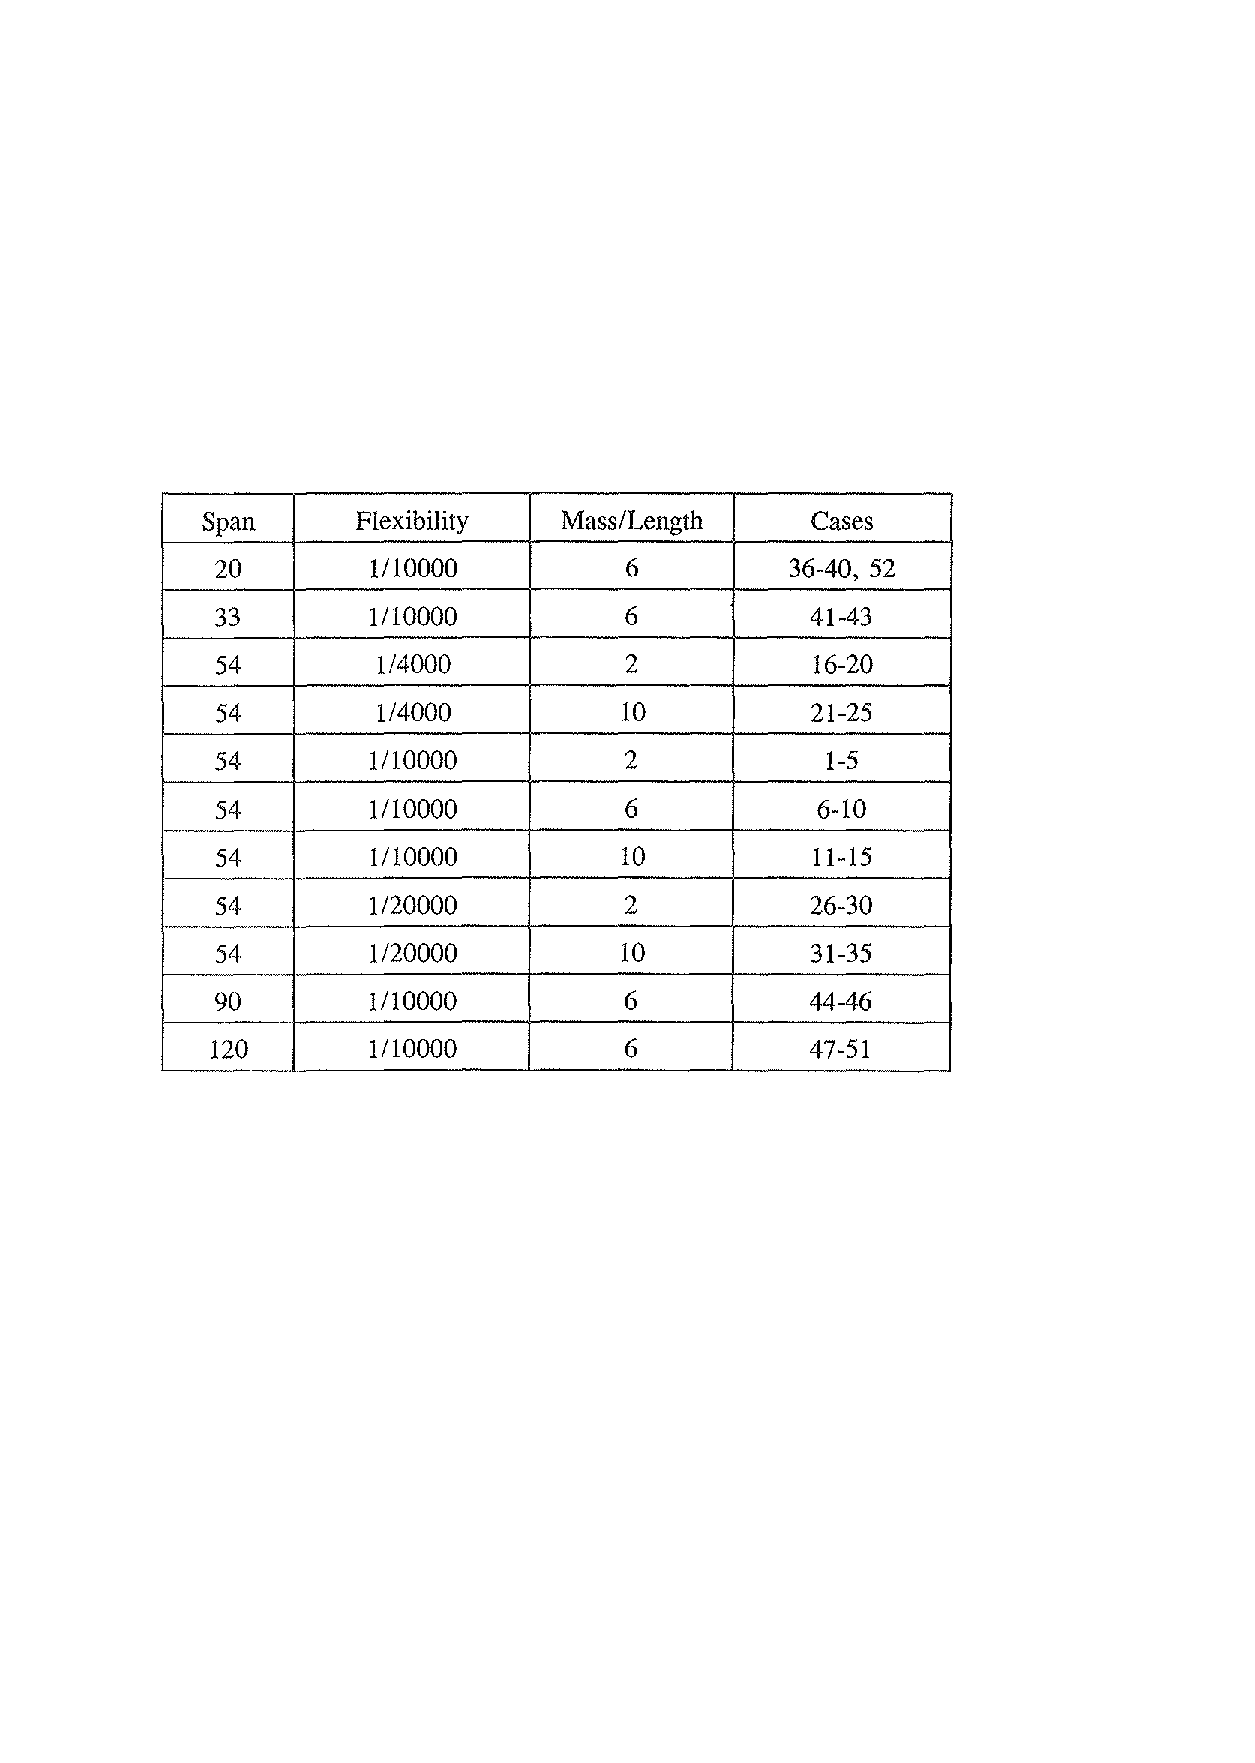
\includegraphics[width=\textwidth]{bridgeparametercombination}
    \caption{Bridge parameter combination}
    \label{fig:bridgeparametercombination}
\end{figure}

\subsubsection{Vehicle parameters}
Three train types are considered: a typical freight train, a typical standard passenger train, and a typical high speed passenger train. Appendix.\ref{app:dt329data} details the parameters used to construct each model. In general, each model consists of a locomotive and a number of identical vehicles appropriate to the train type. The total number of axles in each train is 24. Although effects on the train are only examined on the first vehicle of each type, extra vehicles are added to the train to see what cumulative effects occur to the bridge.

The freight train consists of a British Railways Class 56 locomotive and nine UIC wagons. This has a total length of 131.56 m, which assumes a nominal vehicle coupling distance of 4 m. Runs at 60 km/h and 100 km/h are required.

The standard passenger train consists of an E444 locomotive and five UIC coaches. This has a total length of 143.8 m. It is based on one of two train models used as part of the study of the FS Bridge discussed in report RP 3 of the Committee, differing only by the addition of three extra coaches. This is required to run at 160 km/h and 200 km/h.

The high speed passenger train consists of an ETR500 locomotive and five ETR500 coaches, having a total length of 145.8 m. It is based on the other FS bridge study train model mentioned above, differing from the original by an additional three ETR500 coaches. It is required to run at 300 km/h and 350 km/h.

\subsubsection{Track}

For initial study phase, the track samples used were consistent with each train type. PSD plots of each are shown in Figures \ref{fig:track1} to \ref{fig:track3}. Sample TRACKFRT.DAT was used for all analysis runs for the freight train. This is measured data from a typical BR freight line. Sample TRACKPN.DAT was used for the standard passenger train analysis runs. This is measured data from a part of the BR East Coast main line. Sample TRACKPH.DAT was used for high speed passenger train analysis runs. This is measured data from a typical DB high speed line.

Samples of 500 m were chosen so that there would be 100 m before the bridge and at least 100 m after the bridge for all combinations of span and train length. The initial 100 m is required to check vehicle behaviour on the track irregularity alone, and the portion after the train has left the bridge is required to check that the bridge vibrations decay.

For secondary study phase, the track data used to excite the mathematical models was taken from the British Rail Research library of measured track data. For the viaduct and resonance investigations, the track files used were the same as those used in the first part of the study. For the investigation of the influence of track quality, additional track data was used so as to give the widest possible range of realistic track qualities.

\subsubsection{Contact data}
For each run the same contact data was used, consisting of rails inclined at 1:20, and wheel profiles of conicity of 0.05 (based on standard British Rail 113A rails and PI wheel profiles). The coefficient of friction applied was 0.3.


\subsubsection{Data produced}

For every analysis run the following results were obtained at intervals of 0.01 seconds.

BRIDGE DATA:

Lateral displacement at mid span Lateral acceleration at mid span

\vspace*{\baselineskip}

VEHICLE LATERAL ACCELERATION DATA:

Loco body at leading pivot

Leading coach/wagon body at leading pivot/axle 

Loco leading bogie

Leading coach/wagon leading bogie/axle

\vspace*{\baselineskip}

TOTAL LATERAL FORCE DATA:

Loco leading bogie

Leading coach/wagon leading bogie/axle

\vspace*{\baselineskip}

LATERAL FORCES ON INDIVIDUAL WHEELS

Leading coach/wagon, first axle, left and right wheels 

Leading coach/wagon, second axle, left and right wheels 

Loco, first axle, left and right wheels

Loco, second axle, left and right wheels

\vspace*{\baselineskip}

In addition, for freight train runs, since the locomotive has two bogies of three axles, the forces on the individual wheels of the third axle were also produced.

Peak values for each of the outputs produced for the required ranges were obtained. For bridge outputs, peak values were taken for the period where any part of the train was on the bridge. For loco and leading coach/wagon outputs, peak values were taken whilst the vehicle in question was in contact with the bridge.

Peak values for each output were then read into a spread sheet where they could be compared more easily to check for emerging trends. The spread sheet has been partially automated to produce graphs of a single output for each train type for a single varying bridge parameter, for given values of the other bridge parameters. Figures 4 to 30(\cite{d181dt329}) show typical plots which have been produced in this manner.

\subsection{Investigation of resonance phenomenon studied in DT329}\label{sec:resonance329}

2 types of resonance were studied in DT329, including:

\begin{enumerate}
    \item Resonance caused by axle repeat pattern
    \item Resonance caused by kinematic movement
\end{enumerate}

The summary of these resonances effects are presented in following paragraphs. 

Frequency shift phenomenon is an important characteristics observed from resonance effects lists above. It is explained in Section \ref{sec:apparentshift}

\subsubsection{Resonance caused by axle repeat pattern}

Axle repeat patterns are wavelength phenomena - regardless of vehicle speed, the repeat length is constant. However, since frequency is speed divided by wavelength, the frequency of the axle repeat patterns vary with train speed. A table of axle repeat pattern lengths, and typical frequencies arising from train speed are given in Figure.\ref{tab:329axlerepeat}

By running train at different speeds shows resonance is possible between train and bridge if the axle passing frequency coincides with the first lateral bridge mode. The effect occurring in bridge lateral displacement over a limited frequency range around the resonance frequency.


However, the speed on theory which should yield resonance effect may be different from the speed that actually triggered resonance.

\subsubsection{Resonance caused by kinematic movement of trains} 
Kinematic wavelength also gives rise to frequencies which vary with speed for the same reason. For first lateral bending mode coincidence with kinematic frequency, the kinematic wavelength of each train type had to be established, by running each train at a range of typical operating speeds over a discrete lateral irregularity, and examining the frequency content of the lateral wheel motion. The resulting wavelength ranges are tabulated in Table.\ref{tab:329kinematicwavelength}. See Figure \ref{fig:workflow329kinematic} for an overview of workflow of this study.

The most likely possible resonance in the initial studies to be of this type was between the passenger train at 200 km/h (55.556 m/s) on passenger track and BR PI wheel profiles, and a span of 54 m, stiffness 1/10000, mass/length of 6 tonnes/m. This combination was examined by varying the speed between 55.556 - 64.6 m/s over the span, and by varying the stiffness of the span between 117000 and 1112000 running the train at 55.556 m/s. Another combination was examined - the ETR500 train running between 65 - 80 m/s on high speed track and BR PI wheel profiles, for a span of 38 m, stiffness 1110000, and mass/length 10 tonne/m; the span in this case was chosen to coincide with the kinematic wavelength of the coaches.

Coincidence of vehicle kinematic frequency with bridge first lateral bending mode may cause resonance to occur over a broad range of frequencies to a less pronounced effect than coincidence of axle passing frequencies. Evidence of coincidence of kinematic wavelength with length of span has been found in the lateral acceleration of bridges, but was not demonstrated in the lateral bridge displacement in the cases examined. For short kinematic wavelengths, this effect could not be seen, possibly because of lack of time for the bridge to respond.


\begin{figure}[h]
\centering
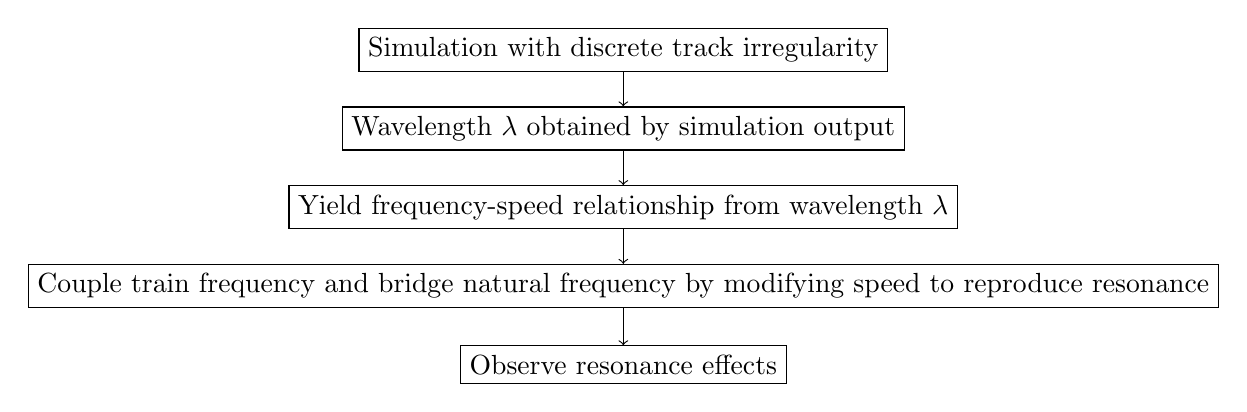
\begin{tikzpicture}
    \node[draw] (simulation1) at (0, 0) {Simulation with discrete track irregularity};

    \node[draw] (analysis) at (0, -1) {Wavelength $\lambda$ obtained by simulation output};

    \node[draw] (yielding) at (0, -2) {Yield frequency-speed relationship from wavelength $\lambda$};

    \node[draw] (matching) at (0,-3) {Couple train frequency and bridge natural frequency by modifying speed to reproduce resonance};

    \node[draw] (observe) at (0, -4) {Observe resonance effects};

    \draw[->] (simulation1) to (analysis);

    \draw[->] (analysis) to (yielding);

    \draw[->] (yielding) to (matching);

    \draw[->] (matching) to (observe);
\end{tikzpicture}
\caption{Workflow of kinematic resonance research}
\label{fig:workflow329kinematic}
\end{figure}

\subsubsection{Apparent shift in resonance frequency}\label{sec:apparentshift}
It is frequently observed in the output of both resonance effects that apparent resonance happens at some frequencies higher than frequencies calculated on theory. This is explained in following quote on \cite[Page 13, Secondary Phase]{d181dt329}. However, the explanation wasn't verified by further studies. They can only be treated as hypothesis.

\begin{quote}
Although the peak mid span displacement was expected to occur at 28.5 mis, it can be seen that for the runs with just the coaches that the peak occurs at about 32 m/s. This is confirmed to be a resonance-type effect rather than a discrete event in the time histories of the runs, a selection of which are shown in Figure C6(Original report), of which an extract of 100-285m follows as Figure C7(Original report). This speed is mid way between axle passing frequency coinciding with first bending mode of the bridge, and kinematic frequency coinciding with the first bending mode. So, the apparent shift in resonant frequency may be due to a combination of these effects (see discussion of kinematic frequency resonance results). However, an alternative explanation may be that as track forces generally increase with speed, the deflection of the span would be expected to increase. If this effect continued through a resonant band, the peak displacement would appear greater at a speed slightly above that calculated for resonance, as sketched in Figure \ref{fig:apparentshift}.
\end{quote}

\begin{figure}[h]
    \centering
    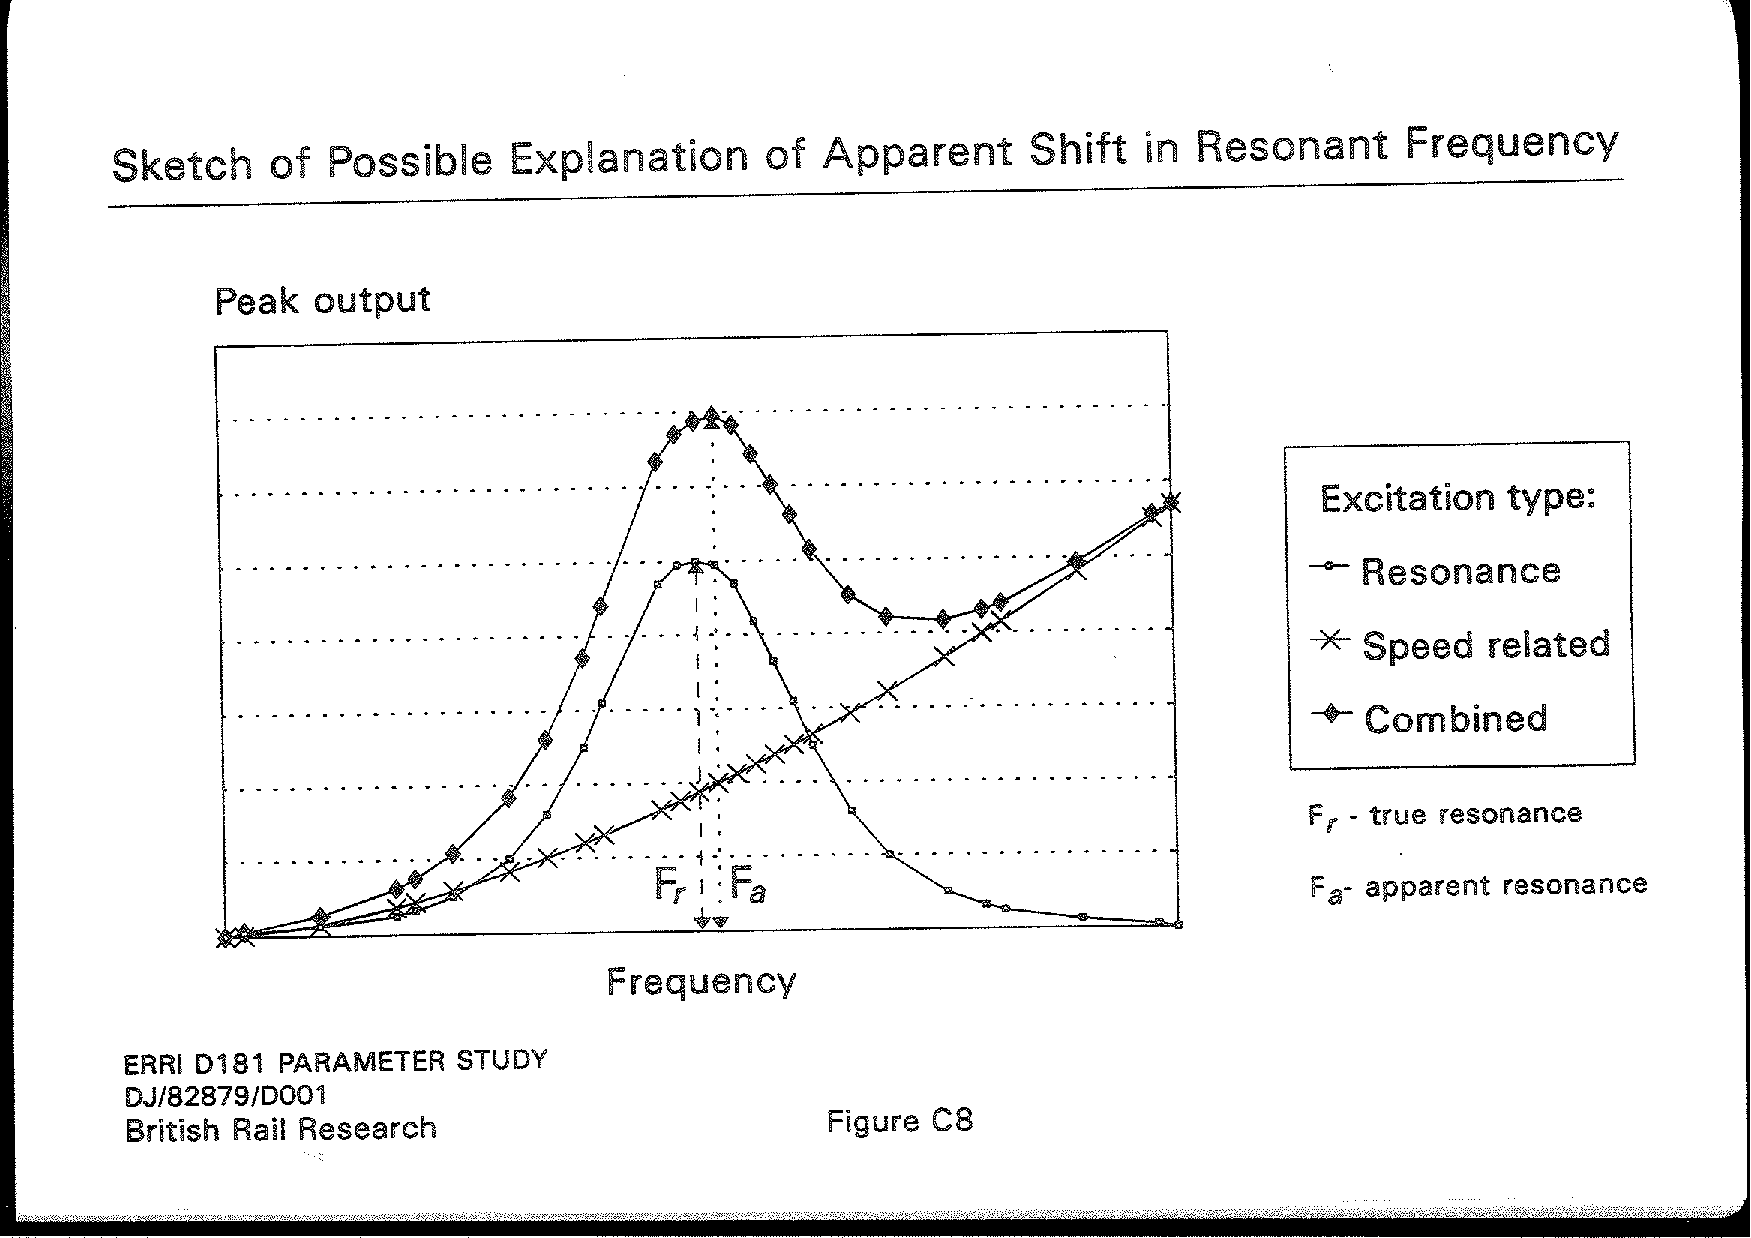
\includegraphics[width=\textwidth]{apparentshift}
    \caption{Sketch of Possible Explanation for Apparent Shift in Resonant Frequency. Extract from \cite[Appendix 2]{d181dt329}}
    \label{fig:apparentshift}
\end{figure}

In the sketch of possible explanation of apparent shift in resonant frequency(Figure \ref{fig:apparentshift}), the combined effect is the superposition of both resonance effect and speed-related effect. Speed-related effect simply increase when speed increase regardless of resonance. Speed is linear to frequency. Thus speed-related effect also simply increase when frequency increases. Resonance effect has an impact where frequency of train and bridge coincides. Speed-related effects is the cause for the frequency shift of combined peak output.

Both explanations indicate that apparent resonance frequency can hardly be predicted. Apparent frequency may even shift into domain lower than theory frequency. 


\section{Investigation of RP6}

\subsection{Debate on proposed 1.2Hz criterion}\label{sec:1.2criterion329}

The value of frequency limit, 1.2Hz is explained in \cite[p3.2: Criterion 2]{d181}:

\begin{quote}
To avoid the occurrence of resonance in the lateral motion of the vehicles due to the lateral motion of the bridge, a limit value lower than the first natural frequency $f_1t$ of the lateral vibration of the span studied should be fixed. The natural frequency for lateral movements is between 0.5 and 0.7 Hz for coaches and between 0.7 and 1 Hz for locomotives. We therefore propose a safety margin $F_{lt} \geq 1.2Hz$

\end{quote}

The original author of report RP6 Graham Scott was contacted to reveal the background of 'natural frequency for lateral movements'. Mr.Scott is still in charge of the development of software VAMPIRE and he's still active in the field. Unfortunately he was unable to remember what did 'natural frequency for lateral movements' stand for in previous quotes since it was written nearly 20 years ago. He passed me to his colleague Alan Minnis for further questions. Mr.Minnis stated following:

\begin{quote}
Looking at the values I think they would refer to typical rigid body modes of a vehicle.  These are independent of speed and a typical passenger coach with air suspension will have a lower sway frequency of around 0.6Hz which is within 0.5-0.7Hz.  Locomotives tend to have a slightly stiffer suspension hence the slightly higher frequency range.
\end{quote}

Mr.Minnis statements, combined with results yielded in supporting parametric report DT329 proves 1.2Hz criterion is aiming to avoid occurrence of resonance. But this isn't a feasible strategy in following reasons:

\begin{enumerate} 
    \item The resonance between rigid body mode of train and first lateral vibration mode of the bridge has never been discussed in all D181 report series. No research proofed this kind of resonance can be critical in real life scenario.

    \item There are lots of evidence can be found in report DT329, showing resonance can happen on a bridge with a first lateral natural frequency even higher than 1.2Hz, which is self-conflicting with 1.2Hz criterion. In fact, the resonance could happen at any frequency on theory. However, the magnitude of resonance effect ranges from less pronounced to more pronounced from case to case.  

    For example, \cite[Page 14,Phase II]{d181dt329} shows resonance occurs on 1.71Hz:
        \begin{quote}
            The first lateral bending mode of this bridge is at 1. 71 Hz. The kinematic wavelength of the passenger coaches is around 34-38 m, giving a kinematic frequency range of 1.46 - 1.63Hz.Speeds of 58.14 m/s(1.53-1.71 Hz)and 64.6m/s(1.7-1.9Hz)were also done. The mid span lateral displacement for each of the time histories are shown in Figure C12(Orignial report). The slowest speed appears to show the greatest resonance.
        \end{quote}
\end{enumerate}

\subsection{Lateral forces on railway bridges}\label{sec:lateralforce329}

\subsubsection{Basic characteristics of lateral force on railway bridges}
It is concluded in initial phase of the study that presence of the bridge doesn't influence the track forces and track quality is a major factor in determining the lateral forces generated by a particular train on \cite[Page 7, Secondary Phase]{d181dt329}



\begin{quote}
    From the initial study [1], it was concluded that the track quality on a bridge is a major factor in determining the lateral forces generated by a particular train. The D181 Committee therefore asked BRR to determine the peak track forces generated over a wide range of track qualities.

    The length of a bridge is small compared to the overall length of a railway track and so track quality on a single bridge may not be representative of that on other bridges on the same route. However the initial study concluded that, in general, the lateral track forces are not influenced by the presence of the bridge.
\end{quote}

The resonance effects mentioned in the previous sections were only observed in deflection and acceleration domain due to the reason that the presence of the bridge doesn't influence the track forces. 


Influence on the total lateral force as a result of hunting of single vehicle bodies were examined. Three parameters were involved in this parametric research. They were vehicle speed, track irregularities deviation and wheel conicity.

Vehicle speed plays a key role. When speed is 60 km/h for freight trains, in the response output, there is very limited influence by increasing both track deviation and conicity. Different conicity tends to yield same force output. Same as track deviation. See Figure B1.

When speed increases, output of different conicity on same track deviation is more scattered. Similarly, increased deviation yields yields greater output. They are two basic trends observed in all output data.

However, it is uncertain which conicity will yield greater output compared to other 2 conicity setups. Surprisingly, in some cases, best maintained wheel profile (effective conicity 0.05) generates greater output than poorly maintained wheels (effective conicity 0.4). See Figure B2. The most obvious case of this kind is freight train running at 100 km/h on track with 5.7mm (approximate) deviation.

Different from conicity, the influence of increasing track deviation is simply predictable. Research report DT329 provided approximate linear function for relationship between lateral force and track deviation. These linear functions can be extracted from plots B1-B30 of DT329.

Since peak force output of 120 km/h freight train and 200 km/h passenger train are close(2\% difference), it is reasonable to conclude that passenger train tends to yield smaller result than freight train at same speed. This is probably due to passenger trains have more sophisticated suspension system designed to suppress lateral motion of the vehicle. Unfortunately, only one speed of 200km/h configuration was available in DT329. But since freight train yields greater output, it is conservative for designer to adopt force output of freight trains for speeds of 60km/h, 100km/h, 120km/h.

It is worthy to point out a suspicious mistake of DT329 in Table.\ref{tab:peaklateralforce}. Report claimed that output data were filtered by statistical analysis. The peak lateral track force was determined from a statistical analysis of lateral track forces as $M \pm 3\sigma$ where $M$ is the mean lateral force value over the segment and $\sigma$ is the standard deviation over the segment. It does not give a true maximum lateral force but on which is greater than 99.5\% of all force values. It is obvious in Table.\ref{tab:peaklateralforce} that output data of 160kN for freight train wagon was not filtered by statistical analysis. It is the greatest value among all raw output data of freight train running at 100 km/h. See Figure B7. This data of 160kN also illustrates that 
peak forces will be influenced by discrete features in the track geometry which may not be reflected thoroughly in the standard deviation. This thesis report suggest substitute 160kN with 80kN(value by approximate observation). See Table.[note1]\ref{tab:peaklateralforce}

\begin{table}[h!]
    \centering
    \caption{Peak Lateral Track Force Over All Track Qualities. Extracted From \cite[Tab. B1]{d181dt329}}
    \begin{tabular}{cccc}
        \hline
        Peak lateral force(kN) & Locomotive Total & Coach/Wagon & Total \\ 
        \hline
        Freight 60 km/h & 50 & 60 & 110\\
        Freight 100 km/h & 90 & 160(\textbf{\textit{80}})$^1$ & 250(\textbf{\textit{170}})$^1$\\
        Freight 120 km/h & 75 & 110 & 185 \\
        Passenger 200 km/h & 140 & 50 & 190 \\
        High Speed 350 km/h & 125 & 125 & 250 \\
        Passenger 200 km/h(worn wheels) & 190 & 80 & 270 \\
        High Speed 350 km/h(worn wheels) & 330 & 225 & 555 \\
        \hline
    \end{tabular}
    \begin{flushleft}
    Note1: Force value 160kN for wagon of freight train running at 100 km/h is not representative. But it is not filtered by statistical analysis. It is advised to substitute 160kN with 80kN. 80kN is obtained by approximate observation of \cite[Figure B7]{d181dt329}. As a result, total force is reduced from 250kN to 170kN.
    \end{flushleft}
    \label{tab:peaklateralforce}
\end{table}

Speed and track quality are two most sensitive parameters. Control of track quality is more advisable compared to control of wheel conicity due to the reason that influence of track quality deviation is simply approximate linear to force output, whereas influence of wheel conicity has an unpredictable characteristic. Moreover, track quality can be controlled by using a maintenance regime.

\subsubsection{Refining of lateral force model}

Figure.\ref{fig:peaklateralforceregression} is created to plot total peak force illustrated in Table.\ref{tab:peaklateralforce}. 5 sets of data available were used to create the plot. 3 of them are data of freight train running at 60km/h, 100km/h and 120km/h. The other 2 sets of data are passenger train running at 200km/h and high speed train running at 350km/h respectively. Data produced with worn wheels profiles are neglected because they are not representative for normally maintained railway vehicles. Adjacent points were connected by solid lines. Different colour stands for different train types. Red lines and dots stand for freight trains. Blue stands for passenger trains and black stands for high speed trains. 

It is indicated that freight trains tends to have the biggest lateral force on track compared to other two kind of trains. And high speed train has lowest lateral force on track. This can be explained by freight trains possessing the most stiff suspension systems, while high speed trains possessing complicated suspension system to suppress lateral motion.

It can also be concluded that the relationship between lateral force and speed is not linear. As a general phenomenon observed, force increment decreases as speed increases. Regressions were made to better illustrate the trend of lateral force increment. Please note these regressions are only sufficient within the speed range plotted.

The first regression made was on freight train because it has the most sets of data. The form of function should satisfy:

\begin{enumerate}  
    \item 0kN lateral force when speed is 0km/h
    \item Simply increasing in value but generally decreasing in increment
\end{enumerate}

Finally function form $F=a*v^b$ is selected because its satisfying characteristics. R language was used to perform regression process. The regression result is also in good likelihood with original data. Achieved convergence tolerance was 2.868e-06. The result is presented in Formula.\ref{for:regressionfreight}. See Appendix.\ref{sec:Rregression} for code.

\begin{equation}
\label{for:regressionfreight}
F_{lf} = 5.2064\cdot v^{0.7495}
\end{equation}

Since 1 set of data is available for passenger train, Formula.\ref{for:regressionfreight} is scaled by a constant factor to create regression for passenger trains. Please note that this regression can not be verified because lack of data. However, since freight train has a greater lateral force then passenger train, it is conservative to adopt lateral force of freight train when calculating consequences related to passenger trains. It is still reasonable to adopt this regression since passenger trains are just simply less stiff than freight trains. 

Unfortunately, conducting such transient simulations is extremely time and resource consuming. It is impossible for this thesis to carry out more simulations to verify the sufficiency of following scaled regression. More data on passenger train and high speed train is recommended to be produced by future researches.

The scale factor $k_{pf}$ is obtained by comparing force value yielded by Formula.\ref{for:regressionfreight} at 200km/h and original passenger train force(190kN) data at 200km/h.

$$k_{pf} = \frac{190}{a_{lf}\cdot 200^{b_{lf}}}$$
$$a_{lp} = a_{lf}\cdot k_{pf}$$
merge above two equations, yield
$$a_{lp} = \frac{190}{200^{b_{lf}}} = \frac{190}{200^{0.7495}} \approx 3.58$$

and 

$$F_{lp} = a_{lp}\cdot v^{0.7495}$$

thus

\begin{equation}\label{for:regressionpassenger}
F_{lp} = 3.58\cdot v^{0.7495}
\end{equation}

Lateral force for high speed train were obtained in same manner. The scale factor $k_{hf}$ is obtained by comparing force value yielded by Formula.\ref{for:regressionfreight} at 350km/h and original high speed train force(250kN) data at 350km/h.

$$k_{hf} = \frac{250}{a_{lf}\cdot 350^{b_{lf}}}$$
$$a_{lh} = a_{lf}\cdot k_{hf}$$
merge above two equations, yield
$$a_{lh} = \frac{250}{350^{b_{lf}}} = \frac{250}{350^{0.7495}} \approx 3.10$$

and 

$$F_{lh} = a_{lh}\cdot v^{0.7495}$$
thus

\begin{equation}\label{for:regressionhighspeed}
F_{lh} = 3.10\cdot v^{0.7495}
\end{equation}


\begin{figure}[h]
    \centering
    \begin{tikzpicture}
    \begin{axis}[
    % title = {Peak lateral track forces over all track qualities(worn profile scenario neglected)},
    xlabel={$v(km/s)$},
    ylabel={$F(kN)$},
    ymin = 0, xmin = 0, xmax = 350,
    grid = both,
    ytick = {50,100,...,250},
    xtick = {60,100,120,200,350},
    legend style={
    at={(0,0)},
    anchor=north west,at={(axis description cs:0,-0.1)}}] 
    ]
    \addplot[name path = C,mark=*, green] coordinates {(200,190) (350,250)};
    \addplot[blue,name path = B,mark=*] coordinates {(120,185) (200,190)};
    \addplot[red,name path = A,mark=*] coordinates {(0,0) (60,110) (100,170) (120,185)};
    \addplot[red,name path = D, domain = 0:120, dashed]{5.2064*x^0.7498};
    \addplot[blue,name path = E, domain = 0:200, dashed]{3.58*x^0.7498};
    \addplot[name path = F, domain = 0:350, dashed, green]{3.1*x^0.7498};
    \addplot[domain = 0:350] {100};
    \legend{high speed train, passenger train, freight train, approximate freight train ,approximate passenger train, approximate high speed train, EN1991-2 nosing force},
    \end{axis}
\end{tikzpicture}
\caption{Total peak lateral track forces over all track qualities(worn profile scenario neglected)}
\label{fig:peaklateralforceregression}
\end{figure}

\subsubsection{Application of lateral force model}
Formula\ref{for:regressionfreight},\ref{for:regressionpassenger} and \ref{for:regressionhighspeed} can be used as load forces for different design scenario. However, these loads are normally higher than the load defined in EN1991-2\cite[6.5.2 Nosing force]{EC12}. EN 1991-2 states that the characteristic value of the nosing force shall be taken as $Q_sk = 100 kN$. 

It is worthy to note that although in RP6\cite[Proposed criteria]{d181} several load model with loading magnitude ranging from 70 kN to 270 kN were originally proposed, EN1991-2 uses a single characteristic value of 100 kN for all design scenarios. 


Since no document has explained this modification, this is probably due to the consideration of lower track irregularity deviation during the creation of EN1991-2.

As explained in previous chapter, peak force is generally linear to track standard deviation. Most of the peak lateral force described in DT329 was obtained on track with 7mm standard deviation, while EN13848-5\cite{13848} allows much lower track standard deviation defined in Table \ref{tab:lateraldeviation}. This means peak lateral force on tracks(if maintained according to Eurocode regulations) is also much smaller than peak force obtained in DT329. 

EN1991-2 states the usage of nosing force. See \ref{sec:nosingforce}. Moreover, since loading model is obtained in Figure.\ref{fig:peaklateralforceregression}, a response solution of the bridge can also be obtained. 

This can be done by using the solution in \ref{sec:harmonicloadmodel} and substitute peak force into the formula as the amplitude of harmonic force $F$. Development of this method is presented in Chapter. 
 
It should be noted that the proposed model in RP6, as well as modified model in EN1991-2, is based on the investigation of first two traction units of the train. It is suspected that when bridge is longer, more traction units can run on the bridge simultaneously, introducing bigger force to the bridge. This can lead to a problem that EN1991-2 is non-conservative in the magnitude of nosing force when applied to longer bridges. However, this suspecting hypothesis is not verified in this chapter.  


\section{Conclusion of D181 report series}
The report series managed to create load models for lateral dynamics railway effects. It is worthy to note that the lateral force on the track wasn't influenced by the presence of the bridge. The major influencing parameter for lateral force is track quality and conicity of the wheel profile. 

The resonance phenomenon was successfully reproduced and observed, though its only visible in deflection and acceleration domain. A basic characteristic of resonance, regardless of the type of resonance, is that apparent resonance frequency will shift from resonance frequency calculated on theory. The shift is unpredictable in the sense of both direction and magnitude. The effect related to speed start to creep in when speed is higher, making the effect of resonance less pronounced in higher speed(Figure \ref{fig:apparentshift}). 

Please note that every bridge will always have resonance with running train because axle repeat pattern and kinematic movement are both wavelength phenomenon, which means there is always a speed of train yielding a vibration frequency coincides with the first lateral natural frequency of bridge. However, the effect of resonance happening on long-span bridge is usually unpronounced since the speed of the train is low as 2.5m/s to 14m/s when resonance occurs.  

Some of the conclusion and proposed criteria in RP6 were adopted in Eurocode 1991-2. One of them is 1.2Hz criterion. It was adopted without amending. The other one is lateral force models. They were adopted in a different name as 'nosing force' in \cite[A6.5.2]{EC12}. 

The 1.2Hz criterion was under debate and proofed unreliable in fulfilling its original intention, avoiding occurrence of resonance. There is no research in D181 report series supporting this criterion, nor there exists literature behind the natural frequency of vehicles. This criterion ignored the fact of future bridge designs with long span would certainly have a natural frequency lower than 1.2 Hz. It is advised that Eurocode review this criterion and revise it.